\documentclass[journal=jacsat,manuscript=article]{achemso}

%%%%%%%%%%%%%%%%%%%%%%%%%%%%%%%%%%%%%%%%%%%%%%%%%%%%%%%%%%%%%%%%%%%%%
%% Place any additional packages needed here.  Only include packages
%% which are essential, to avoid problems later. Do NOT use any
%% packages which require e-TeX (for example etoolbox): the e-TeX
%% extensions are not currently available on the ACS conversion
%% servers.
%%%%%%%%%%%%%%%%%%%%%%%%%%%%%%%%%%%%%%%%%%%%%%%%%%%%%%%%%%%%%%%%%%%%%
\usepackage[version=3]{mhchem} % Formula subscripts using \ce{}

%%%%%%%%%%%%%%%%%%%%%%%%%%%%%%%%%%%%%%%%%%%%%%%%%%%%%%%%%%%%%%%%%%%%%
%% If issues arise when submitting your manuscript, you may want to
%% un-comment the next line.  This provides information on the
%% version of every file you have used.
%%%%%%%%%%%%%%%%%%%%%%%%%%%%%%%%%%%%%%%%%%%%%%%%%%%%%%%%%%%%%%%%%%%%%
%%\listfiles

%%%%%%%%%%%%%%%%%%%%%%%%%%%%%%%%%%%%%%%%%%%%%%%%%%%%%%%%%%%%%%%%%%%%%
%% Place any additional macros here.  Please use \newcommand* where
%% possible, and avoid layout-changing macros (which are not used
%% when typesetting).
%%%%%%%%%%%%%%%%%%%%%%%%%%%%%%%%%%%%%%%%%%%%%%%%%%%%%%%%%%%%%%%%%%%%%
\newcommand*\mycommand[1]{\texttt{\emph{#1}}}
\newcommand{\bfv}[1]{{\mbox{\boldmath{$#1$}}}}
\newcommand{\x}{\bfv{x}}
\usepackage{xr}
\makeatletter
\newcommand*{\addFileDependency}[1]{% argument=file name and extension
  \typeout{(#1)}
  \@addtofilelist{#1}
  \IfFileExists{#1}{}{\typeout{No file #1.}}
}
\makeatother

\newcommand*{\myexternaldocument}[1]{%
    \externaldocument{#1}%
    \addFileDependency{#1.tex}%
    \addFileDependency{#1.aux}%
}

\myexternaldocument{main}
%%%%%%%%%%%%%%%%%%%%%%%%%%%%%%%%%%%%%%%%%%%%%%%%%%%%%%%%%%%%%%%%%%%%%
%% Meta-data block
%% ---------------
%% Each author should be given as a separate \author command.
%%
%% Corresponding authors should have an e-mail given after the author
%% name as an \email command. Phone and fax numbers can be given
%% using \phone and \fax, respectively; this information is optional.
%%
%% The affiliation of authors is given after the authors; each
%% \affiliation command applies to all preceding authors not already
%% assigned an affiliation.
%%
%% The affiliation takes an option argument for the short name.  This
%% will typically be something like "University of Somewhere".
%%
%% The \altaffiliation macro should be used for new address, etc.
%% On the other hand, \alsoaffiliation is used on a per author basis
%% when authors are associated with multiple institutions.
%%%%%%%%%%%%%%%%%%%%%%%%%%%%%%%%%%%%%%%%%%%%%%%%%%%%%%%%%%%%%%%%%%%%%
\author{Wei-Tse Hsu}
\affiliation{Department of Chemical and Biological Engineering, University of Colorado Boulder, Boulder, CO 80305}
\author{Valerio Piomponi}
\affiliation{Scuola Internazionale Superiore di Studi Avanzati, Trieste, Italy}
\author{Pascal T. Merz}
\affiliation{Department of Chemical and Biological Engineering, University of Colorado Boulder, Boulder, CO 80305}
\author{Giovanni Bussi}
\affiliation{Scuola Internazionale Superiore di Studi Avanzati, Trieste, Italy}
\author{Michael R. Shirts}
\affiliation{Department of Chemical and Biological Engineering, University of Colorado Boulder, Boulder, CO 80305}
\email{michael.shirts@colorado.edu}

%%%%%%%%%%%%%%%%%%%%%%%%%%%%%%%%%%%%%%%%%%%%%%%%%%%%%%%%%%%%%%%%%%%%%
%% The document title should be given as usual. Some journals require
%% a running title from the author: this should be supplied as an
%% optional argument to \title.
%%%%%%%%%%%%%%%%%%%%%%%%%%%%%%%%%%%%%%%%%%%%%%%%%%%%%%%%%%%%%%%%%%%%%
\title
  {Supporting Information: Adding alchemical variables to metadynamics to enhance sampling in free energy calculations}

%%%%%%%%%%%%%%%%%%%%%%%%%%%%%%%%%%%%%%%%%%%%%%%%%%%%%%%%%%%%%%%%%%%%%
%% Some journals require a list of abbreviations or keywords to be
%% supplied. These should be set up here, and will be printed after
%% the title and author information, if needed.
%%%%%%%%%%%%%%%%%%%%%%%%%%%%%%%%%%%%%%%%%%%%%%%%%%%%%%%%%%%%%%%%%%%%%
% \abbreviations{IR,NMR,UV}
%\keywords{American Chemical Society, \LaTeX}

%%%%%%%%%%%%%%%%%%%%%%%%%%%%%%%%%%%%%%%%%%%%%%%%%%%%%%%%%%%%%%%%%%%%%
%% The manuscript does not need to include \maketitle, which is
%% executed automatically.
%%%%%%%%%%%%%%%%%%%%%%%%%%%%%%%%%%%%%%%%%%%%%%%%%%%%%%%%%%%%%%%%%%%%%
\begin{document}

% \clearpage
\section{Comparison of methylation free energy calculations with dynamic and static biases}
% We should include the lengths of the simulations using the dynamic bias and mention the adopted truncation fraction, average fraction, number of blocks in block bootstrapping, number of iteration for each data point. We should also explain the meaning of the 4th point by explicitly stating what values the 4th point took the difference from. (Like what is done in the section of free energy calculations for the last system in the main text.) 
As a supplementary information, we show the free energy calculations with dynamic bias for the nucleotide and duplex systems. These calculations are done in comparison with the free energy differences computed with static bias presented in the main text. Specifically, simulations at dynamic bias were elongated up to 160 ns. For analysis, the first 60 ns were discarded, and the bias averaged over the remaining 100 ns was used to compute weights. Different numbers of blocks ranging 2 to 1000 were used to construct histograms in block boostrapping (200 iterations) and the largest uncertainty is reported. 

The figure below shows that with dynamic bias, the free energy estimates are more precise (lower statistical errors). This is mostly likely  attributable to the fact that the sampling in the CV space is more diffusive in these systems with dynamically updated weights. However, free energy estimates computed with dynamic bias are less accurate, i.e. the results differ more in alchemical metadynamics than in the case of Hamiltonian replica exchange (HREX). This is probably caused by the dynamic bias adding some small amount of history-dependent blurring. 

To further demonstrate the lower accuracy of the dynamic bias computation, the free energy difference ($\Delta G^{\text{dup, A}}_{syn/anti}$) between the two conformations of adenosine shown in Figure 3A in the main text is calculated. In the work by Piomponi et al.,~\cite{piomponi2022molecular} this value was assumed to be 0 because of the symmetry of the hydrogen atoms H61 and H62. Also, HREX used in the previous work does not have the access to the free energy landscape along the biased torsion, so the relative error is not given for the HREX case. In alchemical metadynamics, $\Delta G^{\text{dup, A}}_{anti/syn}$ was calculated as follows: 
\begin{equation}
    \Delta G^{\text{dup, A}}_{syn/anti}=-\frac{1}{\beta} \ln \left( \frac{\sum_{i \in anti} e^{\beta V^{\text{dup}}_{\text{tot}}(\eta_i, \lambda=0) }}{\sum_{i \in syn} e^{\beta V^{\text{dup}}_{\text{tot}}(\eta_i, \lambda=0)}}\right )
\end{equation} 

For most systems, the general understanding is that using plain metadynamics instead of doing the two-step procedure is better~\cite{bussi2020using}. It is likely the result is system dependent and related to the fact that even without a dynamic bias we can see many of transitions, thus a reasonable statistical error. In this way, we are clearly in the regime where fewer transitions at equilibrium are a safer estimate.

\renewcommand{\thefigure}{S\arabic{figure}}
\begin{figure}[H]
    \centering
    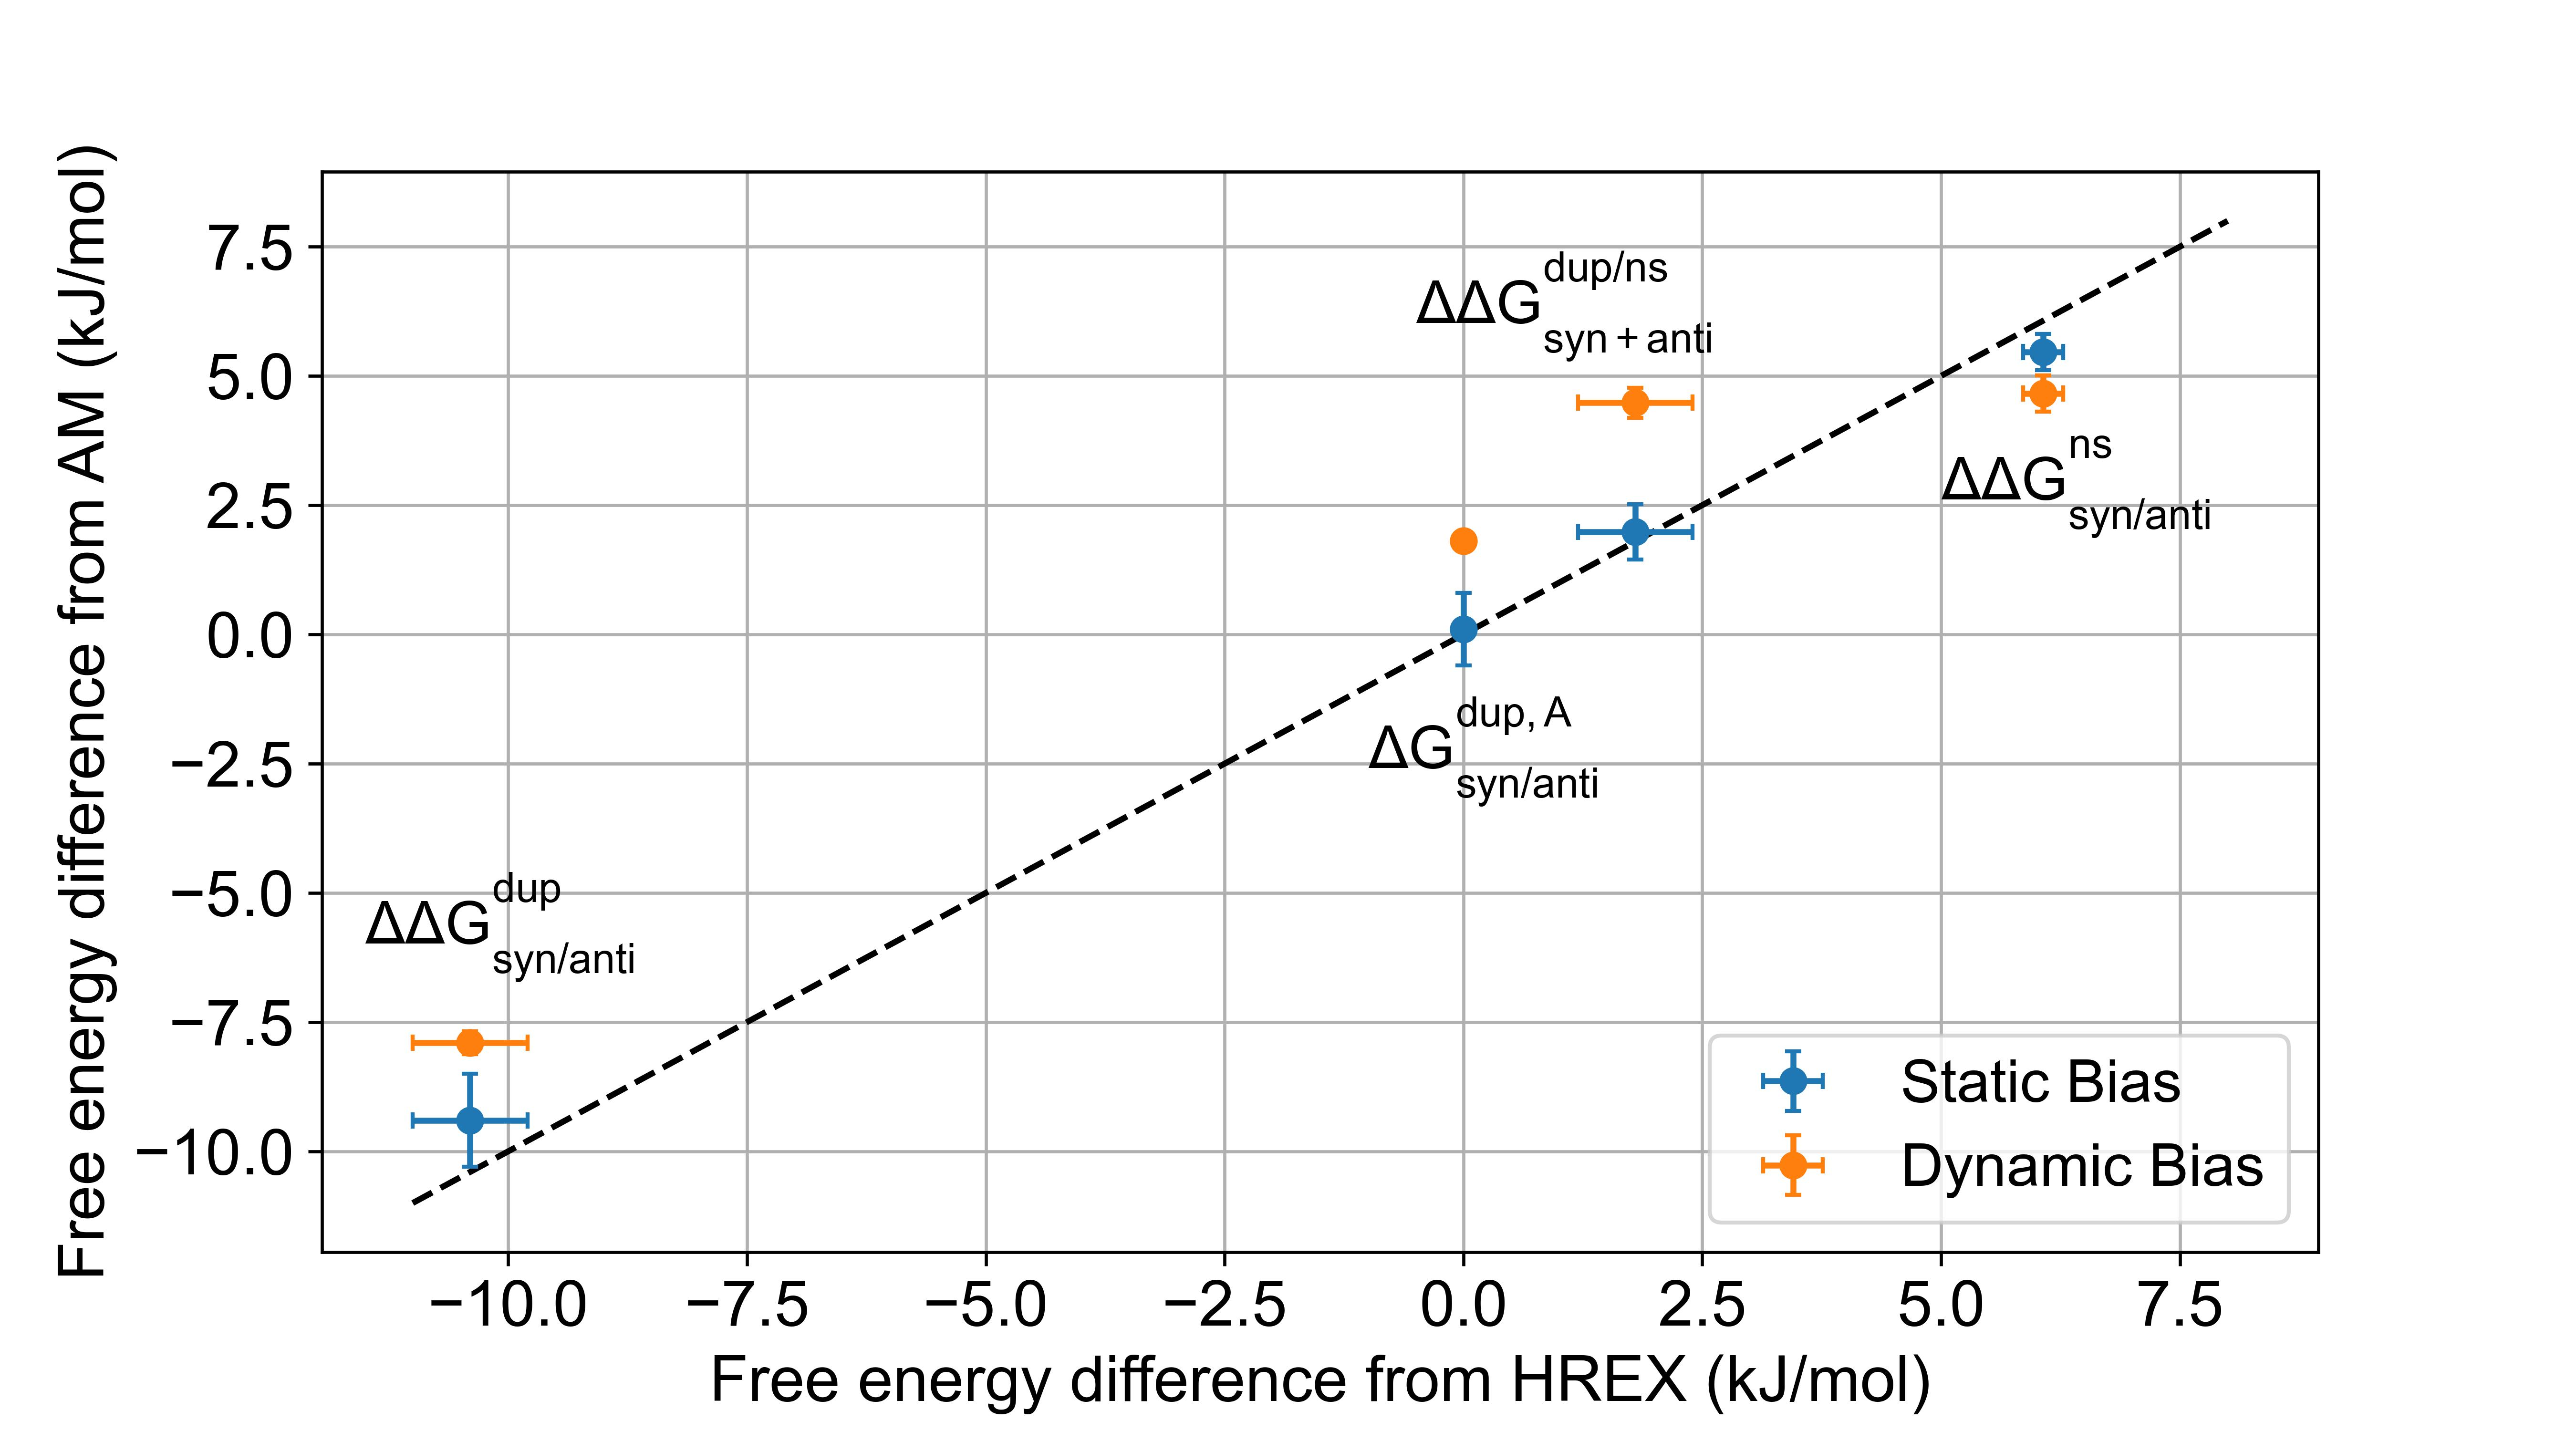
\includegraphics[width=\textwidth]{Figures/m6A_dynamic_static.jpg}   
    \caption{Comparison of free energy differences computed in Ref.~\cite{piomponi2022molecular} with Hamiltonian replica exchange (HREX) and $\Delta \Delta G$ computed with alchemical metadynamics (AM) in this work, for two cases: (1) static bias (as discussed in the main text) and (2) dynamic bias.}
    \label{compare_ACS}
\end{figure}

\section{Supplementary Figures}
\renewcommand{\thefigure}{S\arabic{figure}}
\begin{figure}[H]
    \centering
    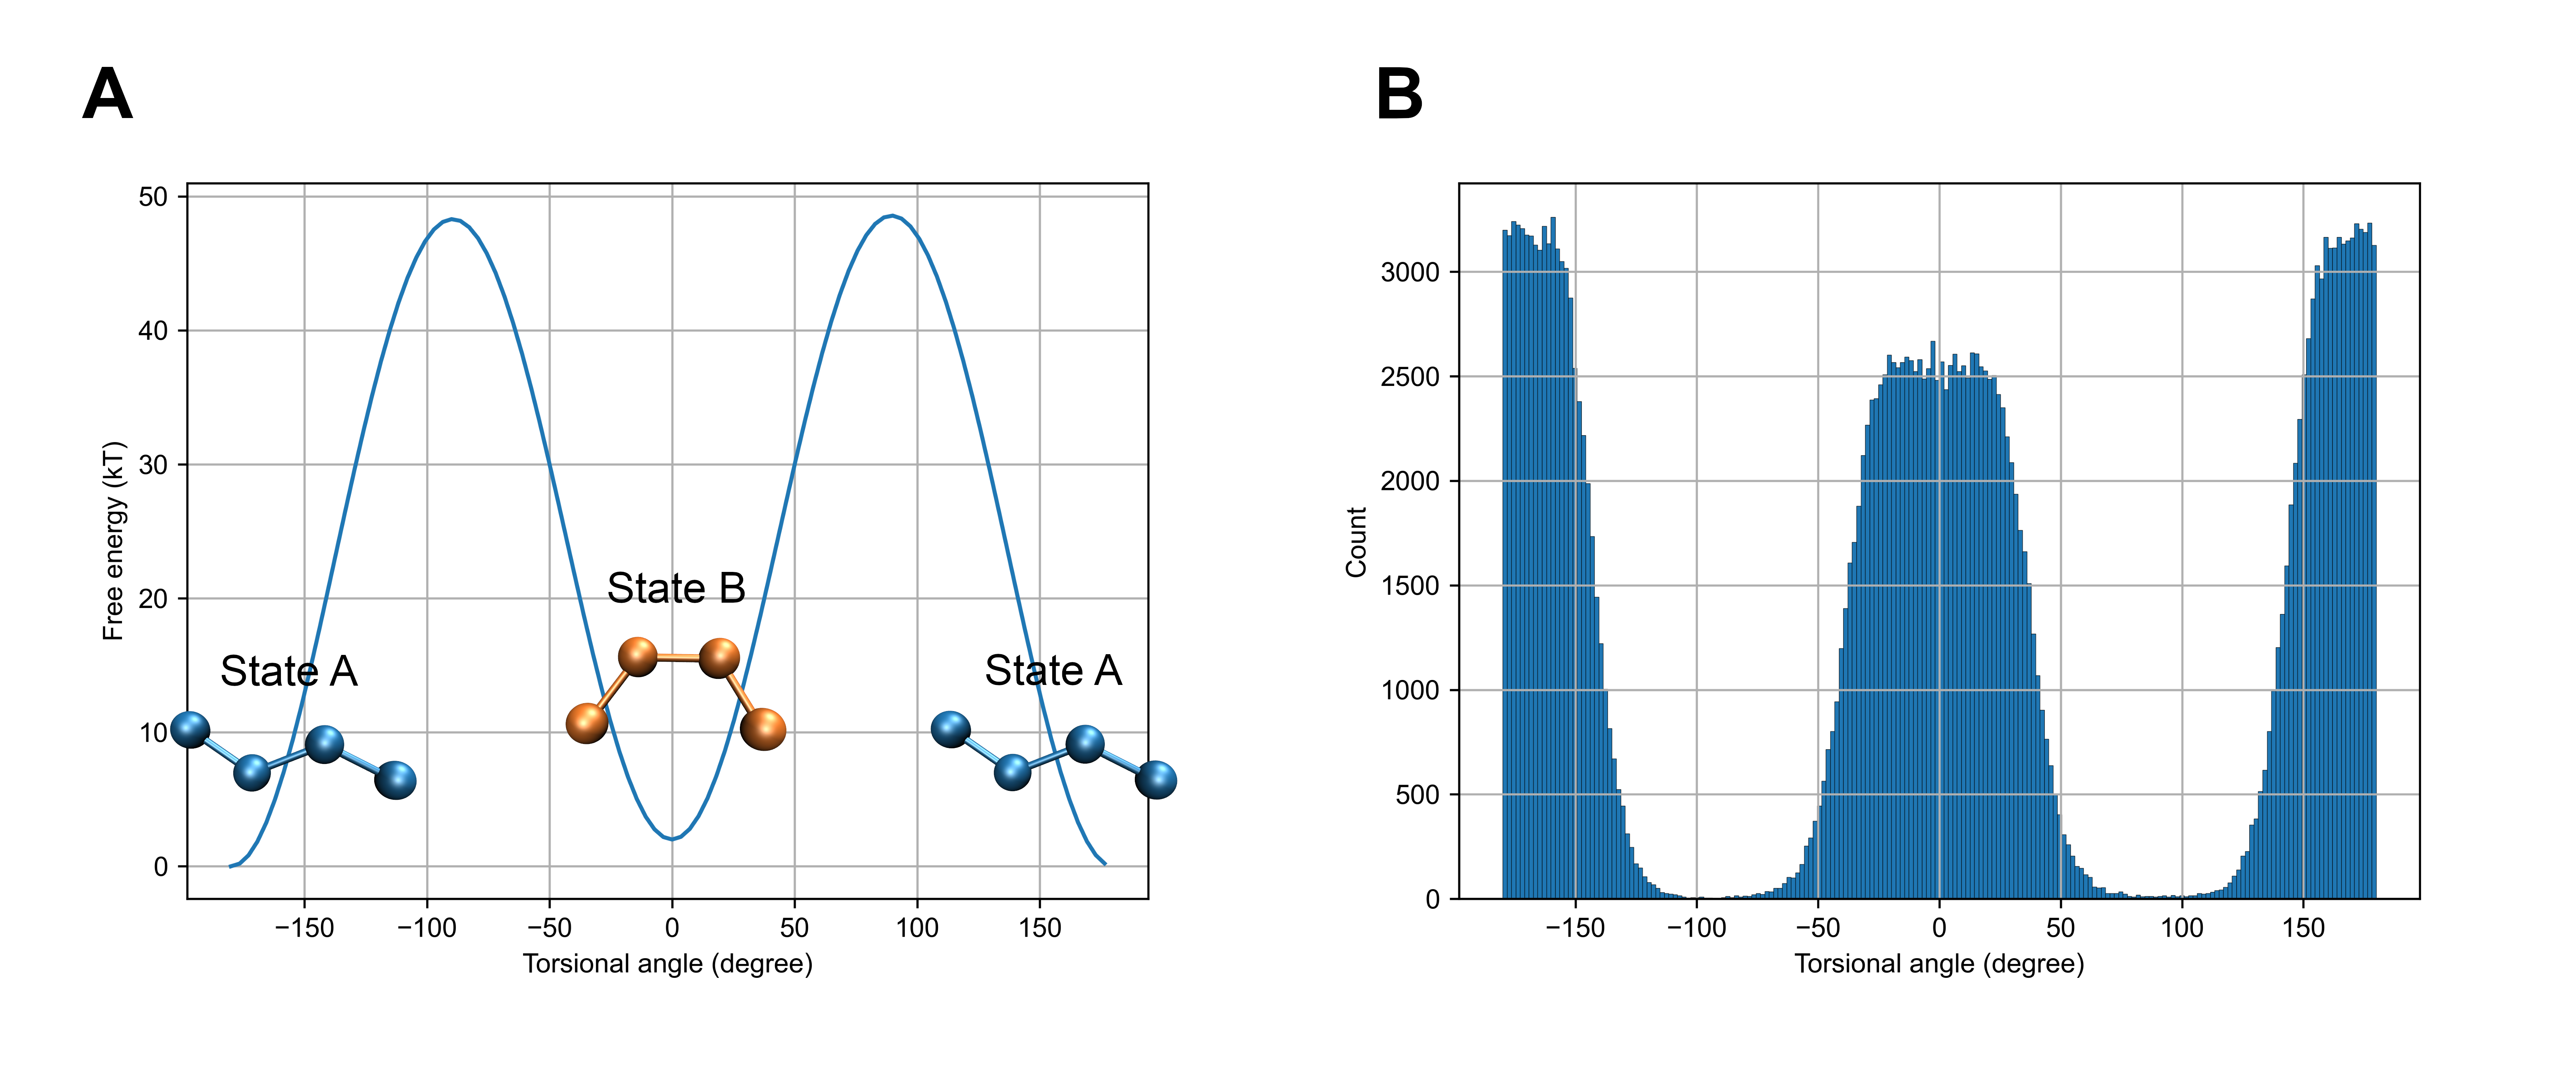
\includegraphics[width=\textwidth]{Figures/sys2_torsional_MetaD_annotated.png}   
    \caption{(A) The free energy profile as a function of the torsional angle. We refer the structures have a torsional angle of $\pm$180$^{\circ}$ and 0$^{\circ}$ as State A (trans isomer) and State B (cis isomer). The torsional free energy barrier starting from either state is around 48.56 kT, which might not be exact since the analysis was done on a very short (5 ns) simulation solely for generating configurations at both states. (B) The histogram of the sampled torsional angle in the torsional metadynamics. As can be seen, the system was able to sample both states frequently during the short simulation.}
    \label{sys2_torsional_MetaD}
\end{figure}

\renewcommand{\thefigure}{S\arabic{figure}}
\begin{figure}[H]
    \centering
    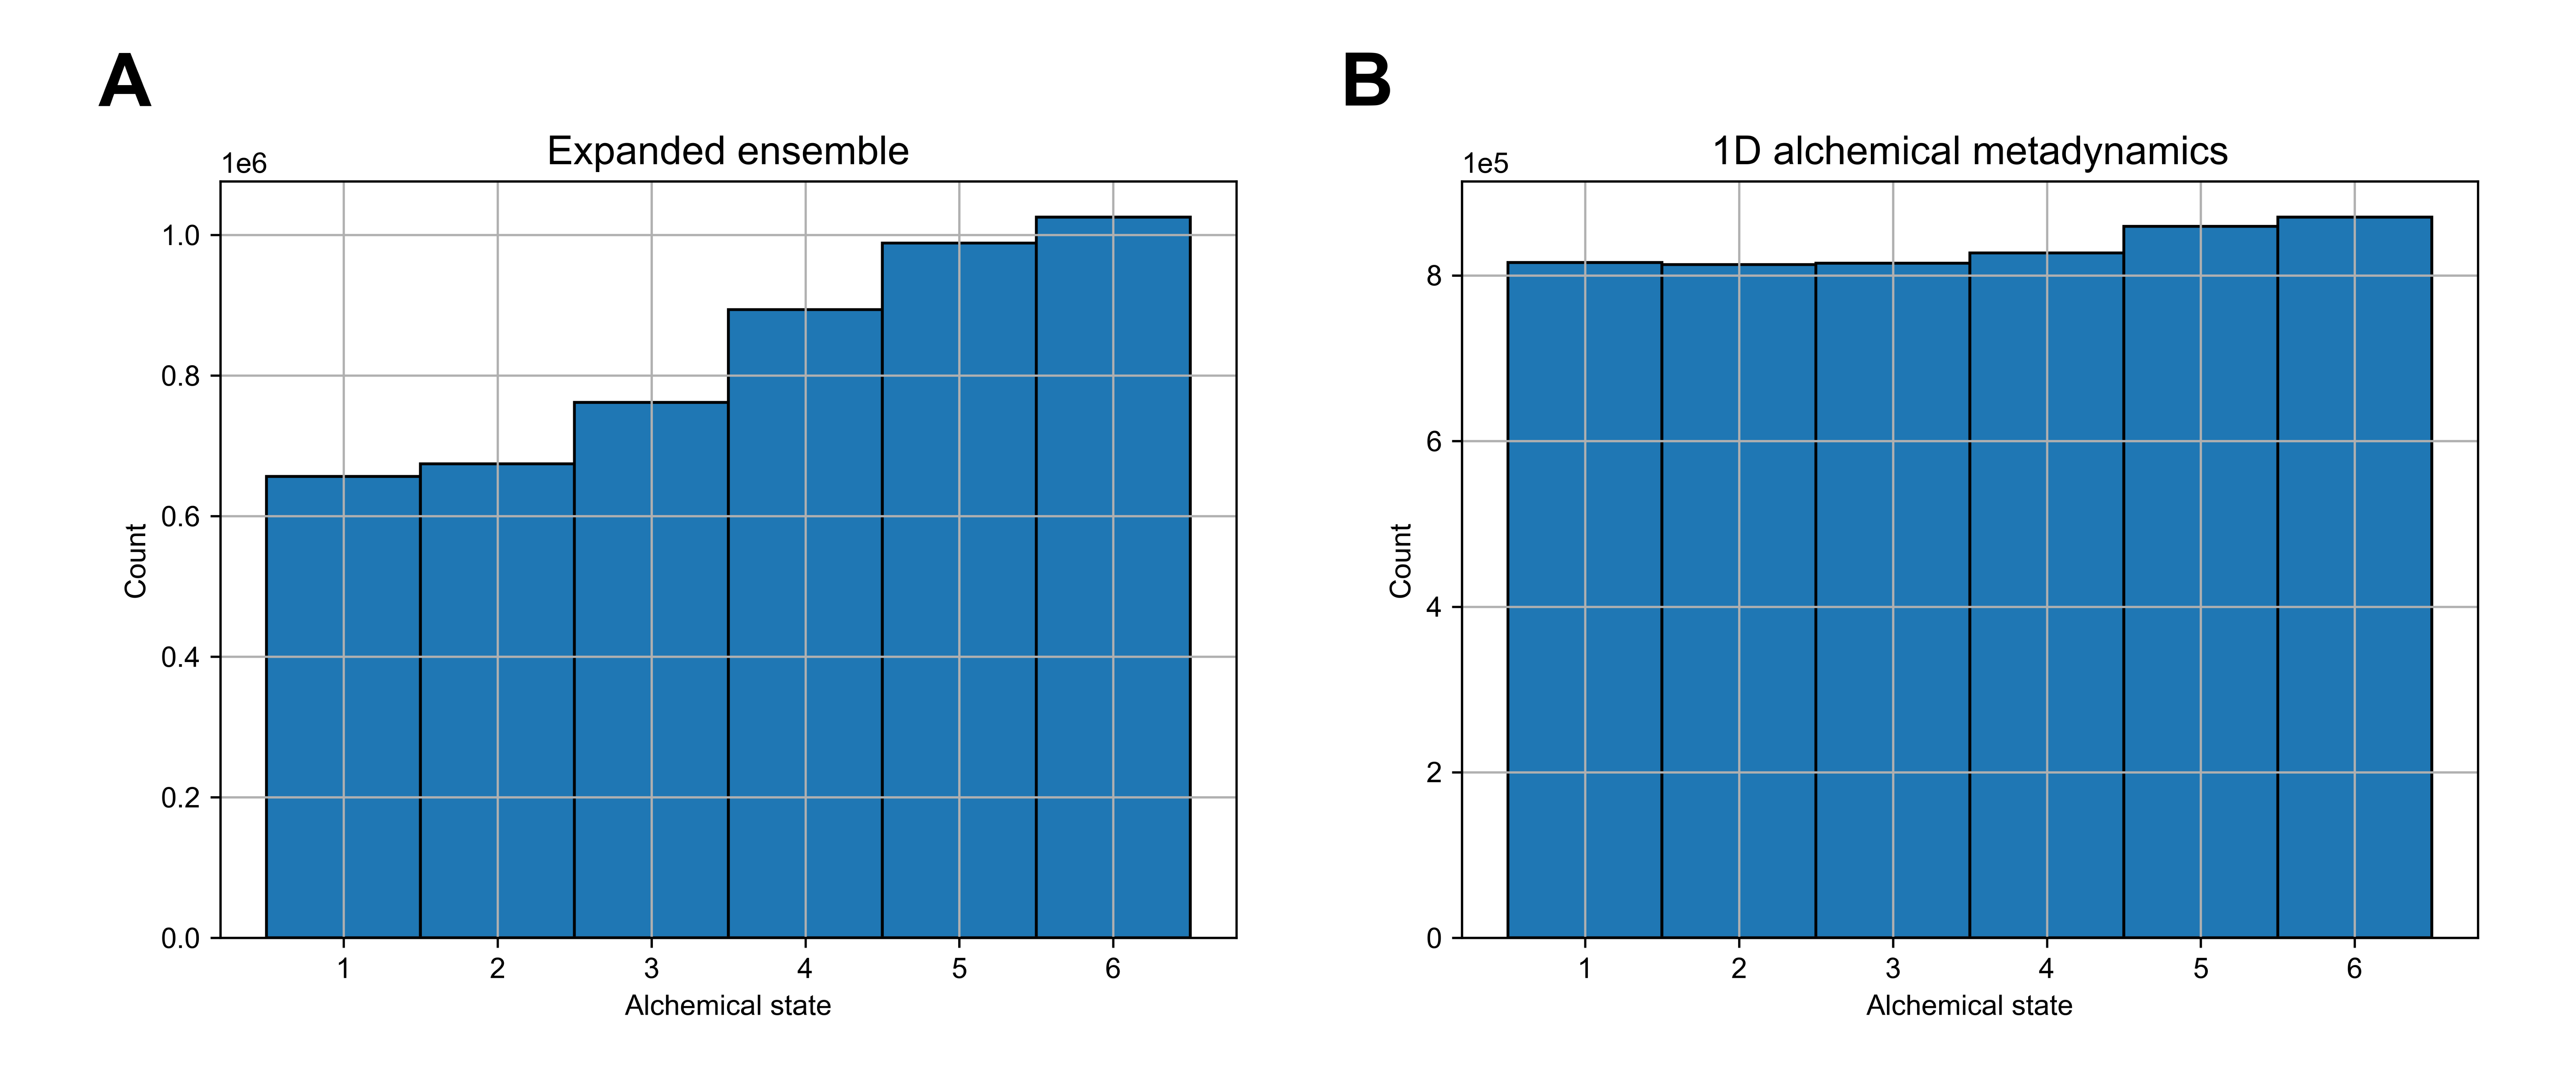
\includegraphics[width=\textwidth]{Figures/sys1_histograms.png}   
    \caption{The histograms of the state visitation in (A) expanded ensemble and (B) 1D alchemical metadynamics of System 1. Both simulations were able to sample all the intermediate states frequently.}
    \label{sys1_hist}
\end{figure}

\renewcommand{\thefigure}{S\arabic{figure}}
\begin{figure}[H]
    \centering
    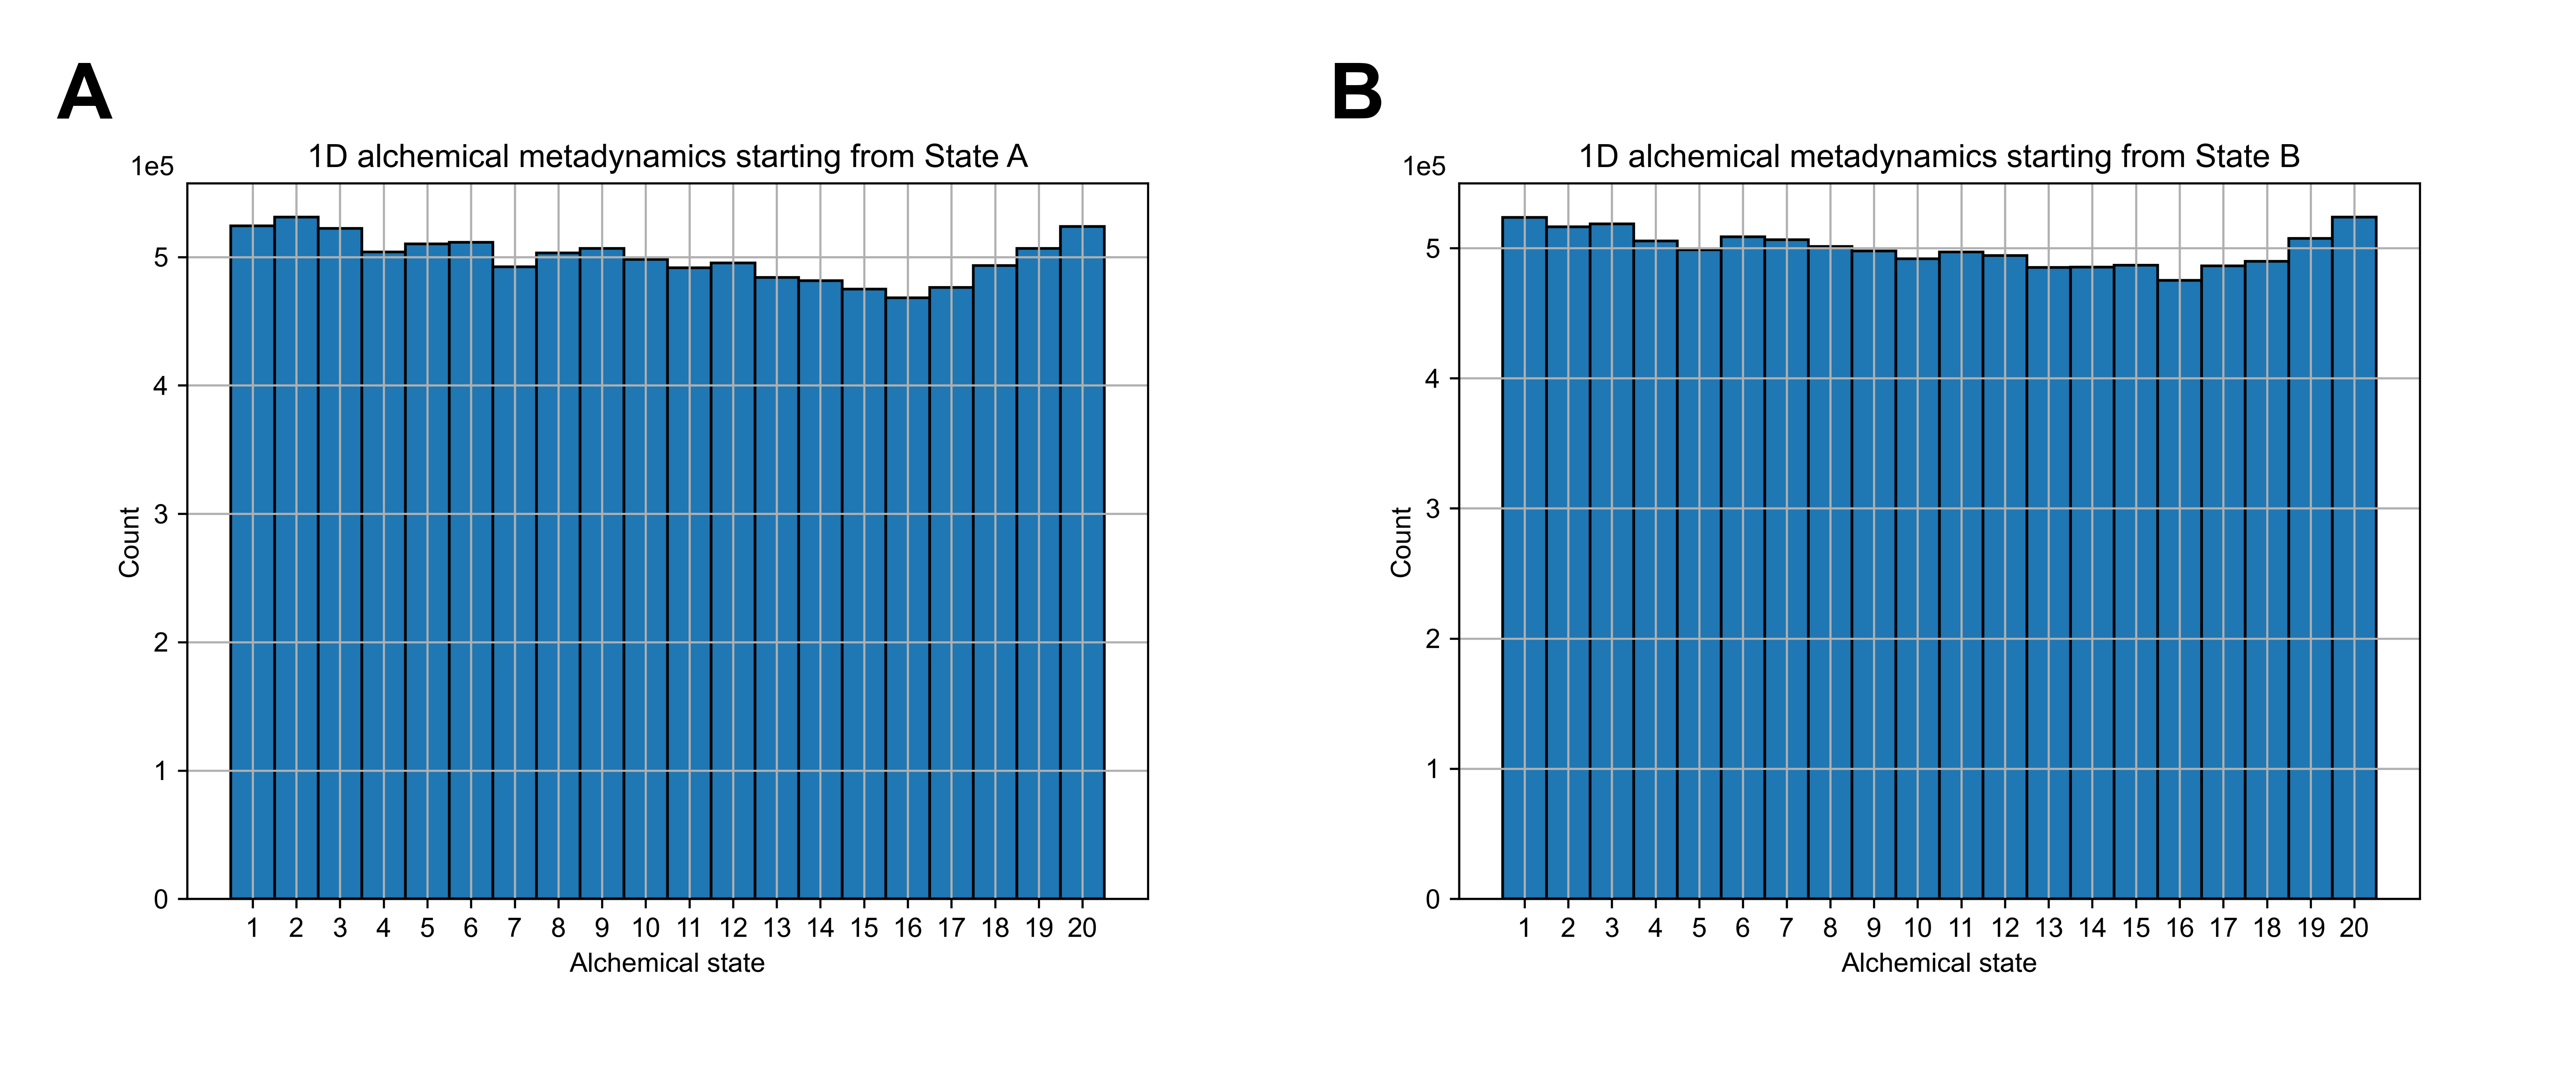
\includegraphics[width=\textwidth]{Figures/1D_lambda_hist.png}   
    \caption{The histograms of the state visitation in the 1D alchemical metadynamics starting from (A) State A and (B) State B. Both simulations were able to freely sample the alchemical space.}
    \label{sys2_1D_hist}
\end{figure}

\renewcommand{\thefigure}{S\arabic{figure}}
\begin{figure}[H]
    \centering
    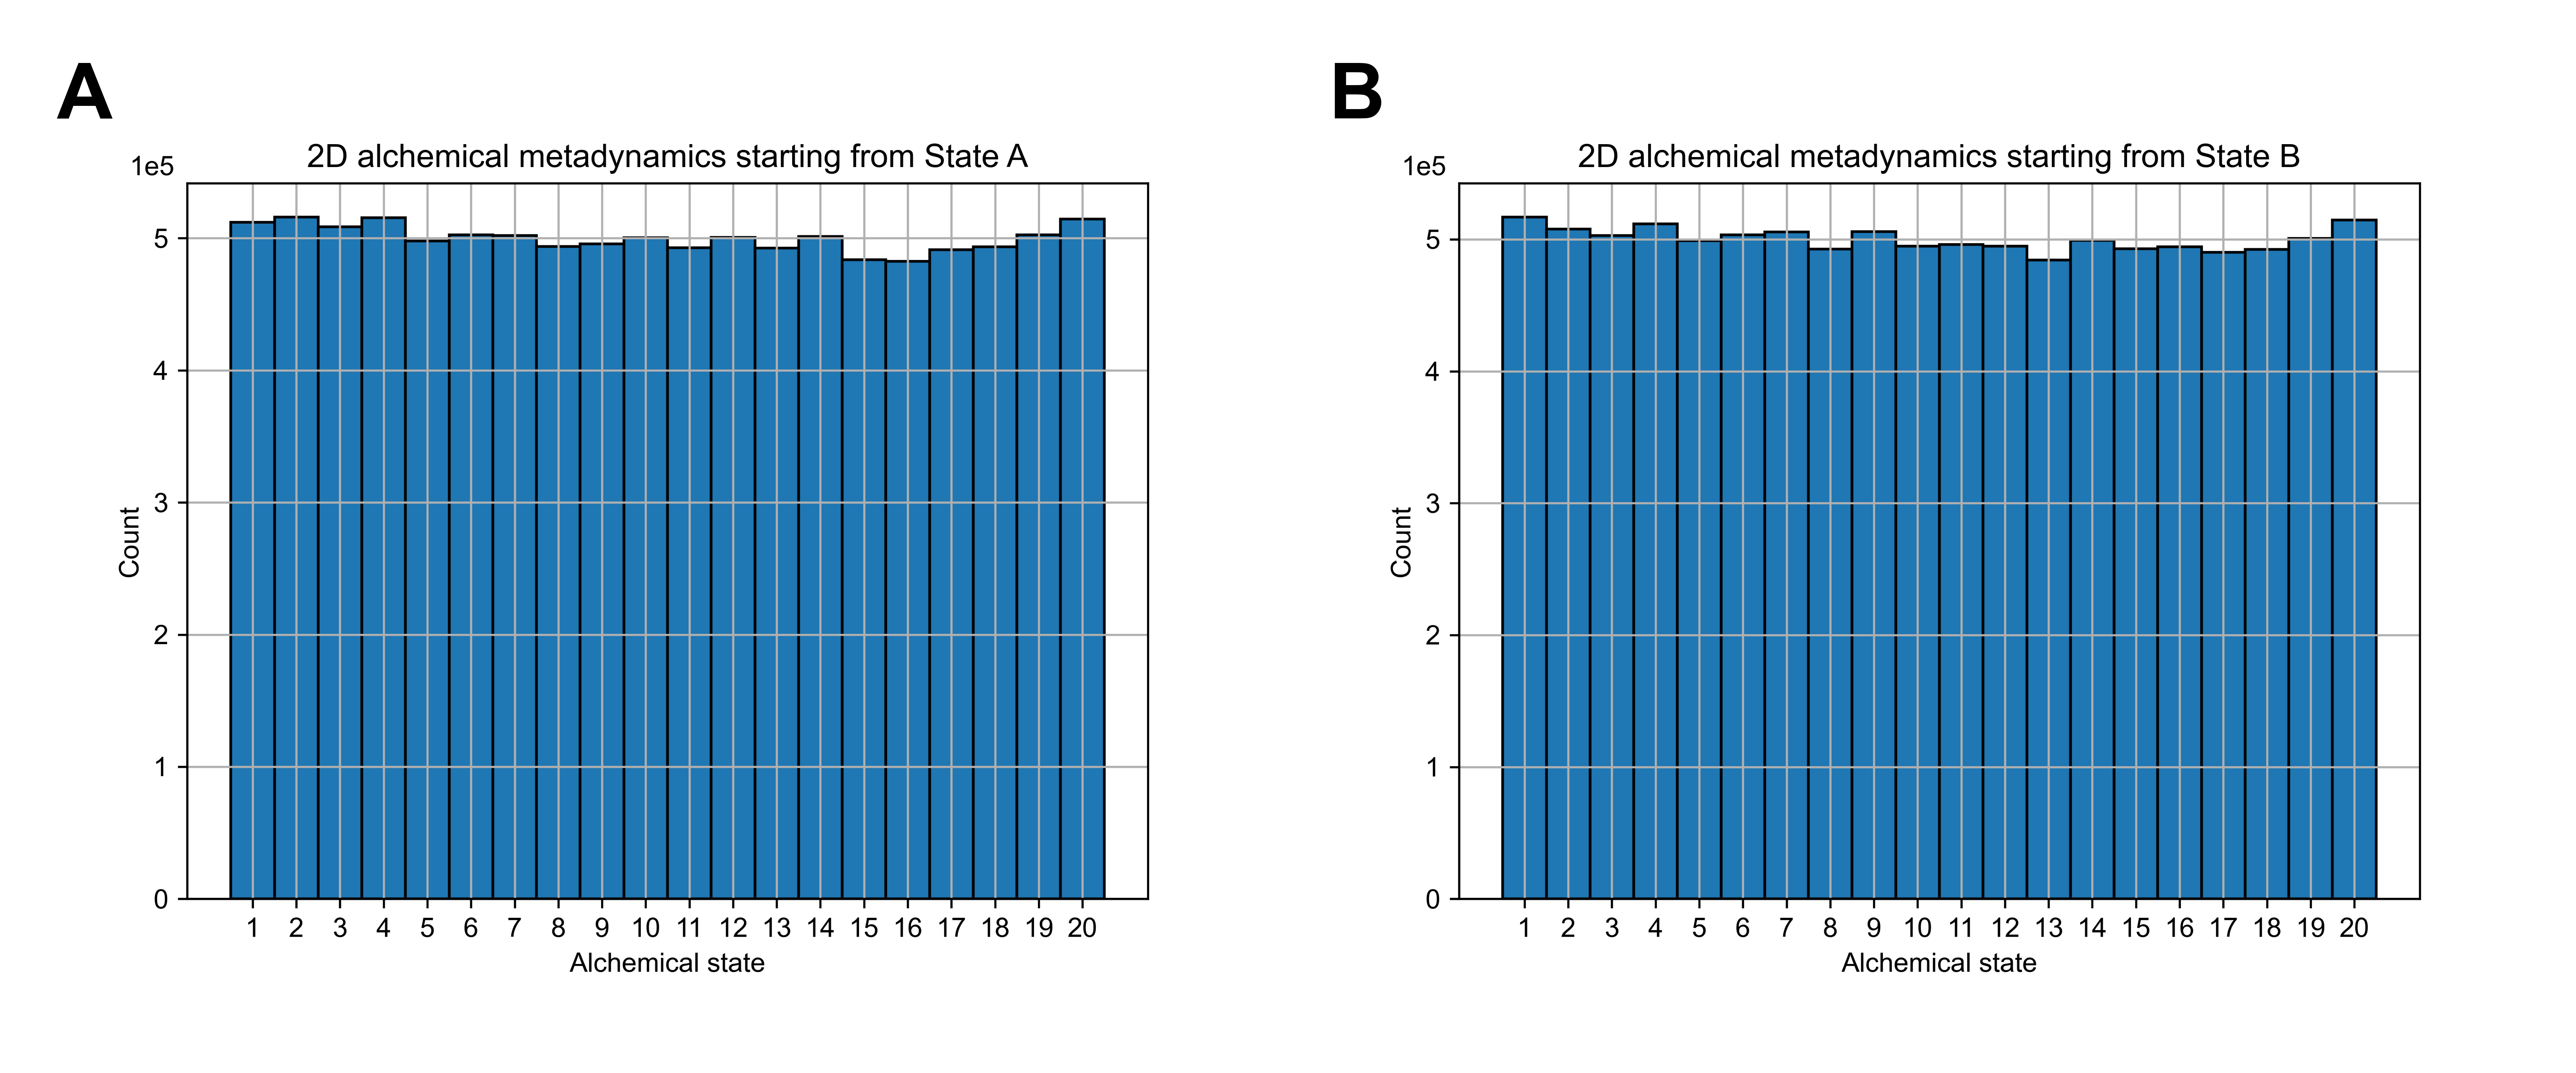
\includegraphics[width=\textwidth]{Figures/2D_lambda_hist.png}   
    \caption{The histograms of the state visitation in the 2D alchemical metadynamics starting from (A) State A and (B) State B. Similar to the two 1D simulations of System 2, both 2D simulations were able to freely sample the alchemical space.}
    \label{sys2_2D_hist}
\end{figure}

\renewcommand{\thefigure}{S\arabic{figure}}
\begin{figure}[H]
    \centering
    \includegraphics[width=\textwidth]{Figures/m6A_sampling.jpg}   
    \caption{(A) Value of the torsional angle N1-C6-N6-C10 as a function of time when the same torsional is used as CV, in a simulation performed at dynamic bias potential. In the 160 ns of simulations, the system only switches once from syn to anti state after about 8 ns and then back to syn after about 60 ns (B) Value of the torsional angle N1-C6-N6-C10 as a function of time when an averaged torsion between  N1-C6-N6-C10,  N1-C6-N6-H62, and  N1-C6-N6-H61 ($+ \pi$) is used as biasing collective variable. In this case, the system becomes diffusive on  N1-C6-N6-C10 after a few ns (C)  N1-C6-N6-C10 vs  N1-C6-N6-H62 when  N1-C6-N6-C10 is used as CV (D) N1-C6-N6-C10 vs  N1-C6-N6-H62 when the averaged torsion is used as CV. The three torsions mentioned here are coupled by an improper torsion that maintains the group C10, N6, H61, and H62 planar. The results shown here demonstrate that the improper torsion is not sufficiently stiff to maintain the consistency between the three torsions when enforcing the barrier crossing. As a consequence, the single N1-C6-N6-C10 torsion is not an optimal CV to allow a proper sampling of the torsional space.}
    \label{sampling}
\end{figure}


\clearpage
%\bibliography{refs}
\documentclass[journal=jacsat,manuscript=article]{achemso}

%%%%%%%%%%%%%%%%%%%%%%%%%%%%%%%%%%%%%%%%%%%%%%%%%%%%%%%%%%%%%%%%%%%%%
%% Place any additional packages needed here.  Only include packages
%% which are essential, to avoid problems later. Do NOT use any
%% packages which require e-TeX (for example etoolbox): the e-TeX
%% extensions are not currently available on the ACS conversion
%% servers.
%%%%%%%%%%%%%%%%%%%%%%%%%%%%%%%%%%%%%%%%%%%%%%%%%%%%%%%%%%%%%%%%%%%%%
\usepackage[version=3]{mhchem} % Formula subscripts using \ce{}

%%%%%%%%%%%%%%%%%%%%%%%%%%%%%%%%%%%%%%%%%%%%%%%%%%%%%%%%%%%%%%%%%%%%%
%% If issues arise when submitting your manuscript, you may want to
%% un-comment the next line.  This provides information on the
%% version of every file you have used.
%%%%%%%%%%%%%%%%%%%%%%%%%%%%%%%%%%%%%%%%%%%%%%%%%%%%%%%%%%%%%%%%%%%%%
%%\listfiles

%%%%%%%%%%%%%%%%%%%%%%%%%%%%%%%%%%%%%%%%%%%%%%%%%%%%%%%%%%%%%%%%%%%%%
%% Place any additional macros here.  Please use \newcommand* where
%% possible, and avoid layout-changing macros (which are not used
%% when typesetting).
%%%%%%%%%%%%%%%%%%%%%%%%%%%%%%%%%%%%%%%%%%%%%%%%%%%%%%%%%%%%%%%%%%%%%
\newcommand*\mycommand[1]{\texttt{\emph{#1}}}
\newcommand{\bfv}[1]{{\mbox{\boldmath{$#1$}}}}
\newcommand{\x}{\bfv{x}}
\usepackage{xr}
\makeatletter
\newcommand*{\addFileDependency}[1]{% argument=file name and extension
  \typeout{(#1)}
  \@addtofilelist{#1}
  \IfFileExists{#1}{}{\typeout{No file #1.}}
}
\makeatother

\newcommand*{\myexternaldocument}[1]{%
    \externaldocument{#1}%
    \addFileDependency{#1.tex}%
    \addFileDependency{#1.aux}%
}

\myexternaldocument{main}
%%%%%%%%%%%%%%%%%%%%%%%%%%%%%%%%%%%%%%%%%%%%%%%%%%%%%%%%%%%%%%%%%%%%%
%% Meta-data block
%% ---------------
%% Each author should be given as a separate \author command.
%%
%% Corresponding authors should have an e-mail given after the author
%% name as an \email command. Phone and fax numbers can be given
%% using \phone and \fax, respectively; this information is optional.
%%
%% The affiliation of authors is given after the authors; each
%% \affiliation command applies to all preceding authors not already
%% assigned an affiliation.
%%
%% The affiliation takes an option argument for the short name.  This
%% will typically be something like "University of Somewhere".
%%
%% The \altaffiliation macro should be used for new address, etc.
%% On the other hand, \alsoaffiliation is used on a per author basis
%% when authors are associated with multiple institutions.
%%%%%%%%%%%%%%%%%%%%%%%%%%%%%%%%%%%%%%%%%%%%%%%%%%%%%%%%%%%%%%%%%%%%%
\author{Wei-Tse Hsu}
\affiliation{Department of Chemical and Biological Engineering, University of Colorado Boulder, Boulder, CO 80305}
\author{Valerio Piomponi}
\affiliation{Scuola Internazionale Superiore di Studi Avanzati, Trieste, Italy}
\author{Pascal T. Merz}
\affiliation{Department of Chemical and Biological Engineering, University of Colorado Boulder, Boulder, CO 80305}
\author{Giovanni Bussi}
\affiliation{Scuola Internazionale Superiore di Studi Avanzati, Trieste, Italy}
\author{Michael R. Shirts}
\affiliation{Department of Chemical and Biological Engineering, University of Colorado Boulder, Boulder, CO 80305}
\email{michael.shirts@colorado.edu}

%%%%%%%%%%%%%%%%%%%%%%%%%%%%%%%%%%%%%%%%%%%%%%%%%%%%%%%%%%%%%%%%%%%%%
%% The document title should be given as usual. Some journals require
%% a running title from the author: this should be supplied as an
%% optional argument to \title.
%%%%%%%%%%%%%%%%%%%%%%%%%%%%%%%%%%%%%%%%%%%%%%%%%%%%%%%%%%%%%%%%%%%%%
\title
  {Supporting Information: Adding alchemical variables to metadynamics to enhance sampling in free energy calculations}

%%%%%%%%%%%%%%%%%%%%%%%%%%%%%%%%%%%%%%%%%%%%%%%%%%%%%%%%%%%%%%%%%%%%%
%% Some journals require a list of abbreviations or keywords to be
%% supplied. These should be set up here, and will be printed after
%% the title and author information, if needed.
%%%%%%%%%%%%%%%%%%%%%%%%%%%%%%%%%%%%%%%%%%%%%%%%%%%%%%%%%%%%%%%%%%%%%
% \abbreviations{IR,NMR,UV}
%\keywords{American Chemical Society, \LaTeX}

%%%%%%%%%%%%%%%%%%%%%%%%%%%%%%%%%%%%%%%%%%%%%%%%%%%%%%%%%%%%%%%%%%%%%
%% The manuscript does not need to include \maketitle, which is
%% executed automatically.
%%%%%%%%%%%%%%%%%%%%%%%%%%%%%%%%%%%%%%%%%%%%%%%%%%%%%%%%%%%%%%%%%%%%%
\begin{document}

% \clearpage
\section{Comparison of methylation free energy calculations with dynamic and static biases}
% We should include the lengths of the simulations using the dynamic bias and mention the adopted truncation fraction, average fraction, number of blocks in block bootstrapping, number of iteration for each data point. We should also explain the meaning of the 4th point by explicitly stating what values the 4th point took the difference from. (Like what is done in the section of free energy calculations for the last system in the main text.) 
As a supplementary information, we show the free energy calculations with dynamic bias for the nucleotide and duplex systems. These calculations are done in comparison with the free energy differences computed with static bias presented in the main text. Specifically, simulations at dynamic bias were elongated up to 160 ns. For analysis, the first 60 ns were discarded, and the bias averaged over the remaining 100 ns was used to compute weights. Different numbers of blocks ranging 2 to 1000 were used to construct histograms in block boostrapping (200 iterations) and the largest uncertainty is reported. 

The figure below shows that with dynamic bias, the free energy estimates are more precise (lower statistical errors). This is mostly likely  attributable to the fact that the sampling in the CV space is more diffusive in these systems with dynamically updated weights. However, free energy estimates computed with dynamic bias are less accurate, i.e. the results differ more in alchemical metadynamics than in the case of Hamiltonian replica exchange (HREX). This is probably caused by the dynamic bias adding some small amount of history-dependent blurring. 

To further demonstrate the lower accuracy of the dynamic bias computation, the free energy difference ($\Delta G^{\text{dup, A}}_{syn/anti}$) between the two conformations of adenosine shown in Figure 3A in the main text is calculated. In the work by Piomponi et al.,~\cite{piomponi2022molecular} this value was assumed to be 0 because of the symmetry of the hydrogen atoms H61 and H62. Also, HREX used in the previous work does not have the access to the free energy landscape along the biased torsion, so the relative error is not given for the HREX case. In alchemical metadynamics, $\Delta G^{\text{dup, A}}_{anti/syn}$ was calculated as follows: 
\begin{equation}
    \Delta G^{\text{dup, A}}_{syn/anti}=-\frac{1}{\beta} \ln \left( \frac{\sum_{i \in anti} e^{\beta V^{\text{dup}}_{\text{tot}}(\eta_i, \lambda=0) }}{\sum_{i \in syn} e^{\beta V^{\text{dup}}_{\text{tot}}(\eta_i, \lambda=0)}}\right )
\end{equation} 

For most systems, the general understanding is that using plain metadynamics instead of doing the two-step procedure is better~\cite{bussi2020using}. It is likely the result is system dependent and related to the fact that even without a dynamic bias we can see many of transitions, thus a reasonable statistical error. In this way, we are clearly in the regime where fewer transitions at equilibrium are a safer estimate.

\renewcommand{\thefigure}{S\arabic{figure}}
\begin{figure}[H]
    \centering
    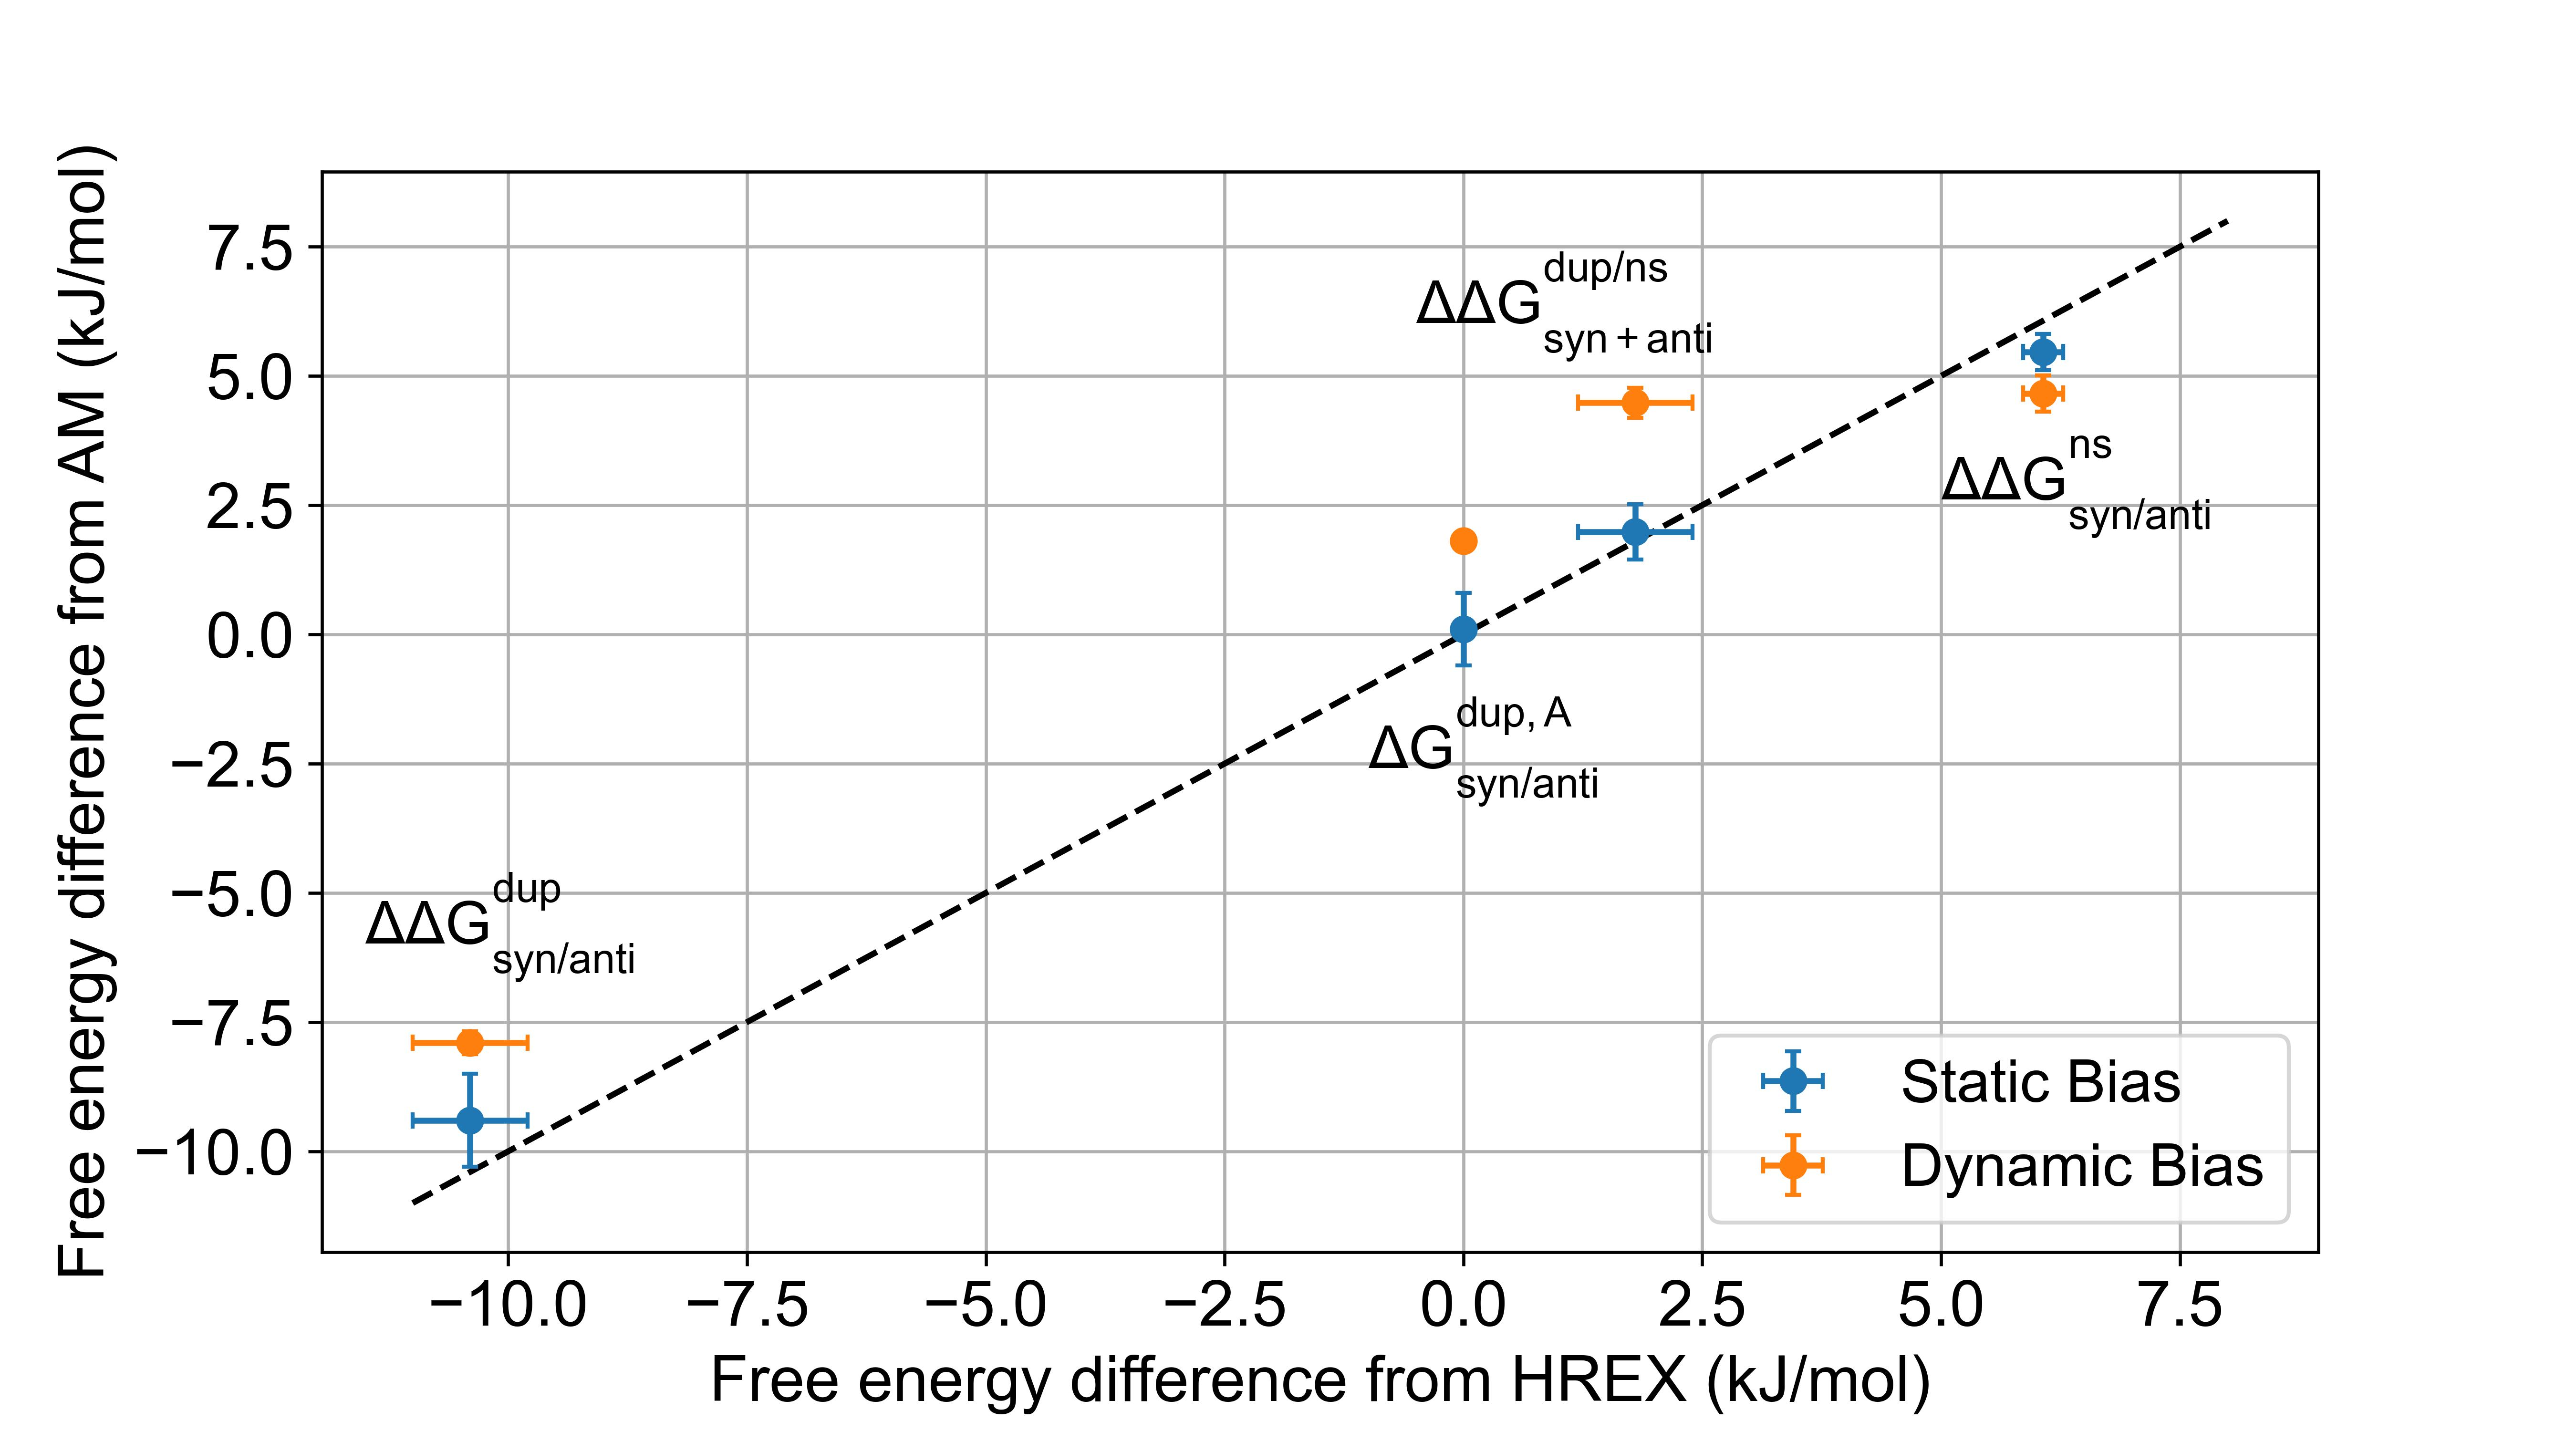
\includegraphics[width=\textwidth]{Figures/m6A_dynamic_static.jpg}   
    \caption{Comparison of free energy differences computed in Ref.~\cite{piomponi2022molecular} with Hamiltonian replica exchange (HREX) and $\Delta \Delta G$ computed with alchemical metadynamics (AM) in this work, for two cases: (1) static bias (as discussed in the main text) and (2) dynamic bias.}
    \label{compare_ACS}
\end{figure}

\section{Supplementary Figures}
\renewcommand{\thefigure}{S\arabic{figure}}
\begin{figure}[H]
    \centering
    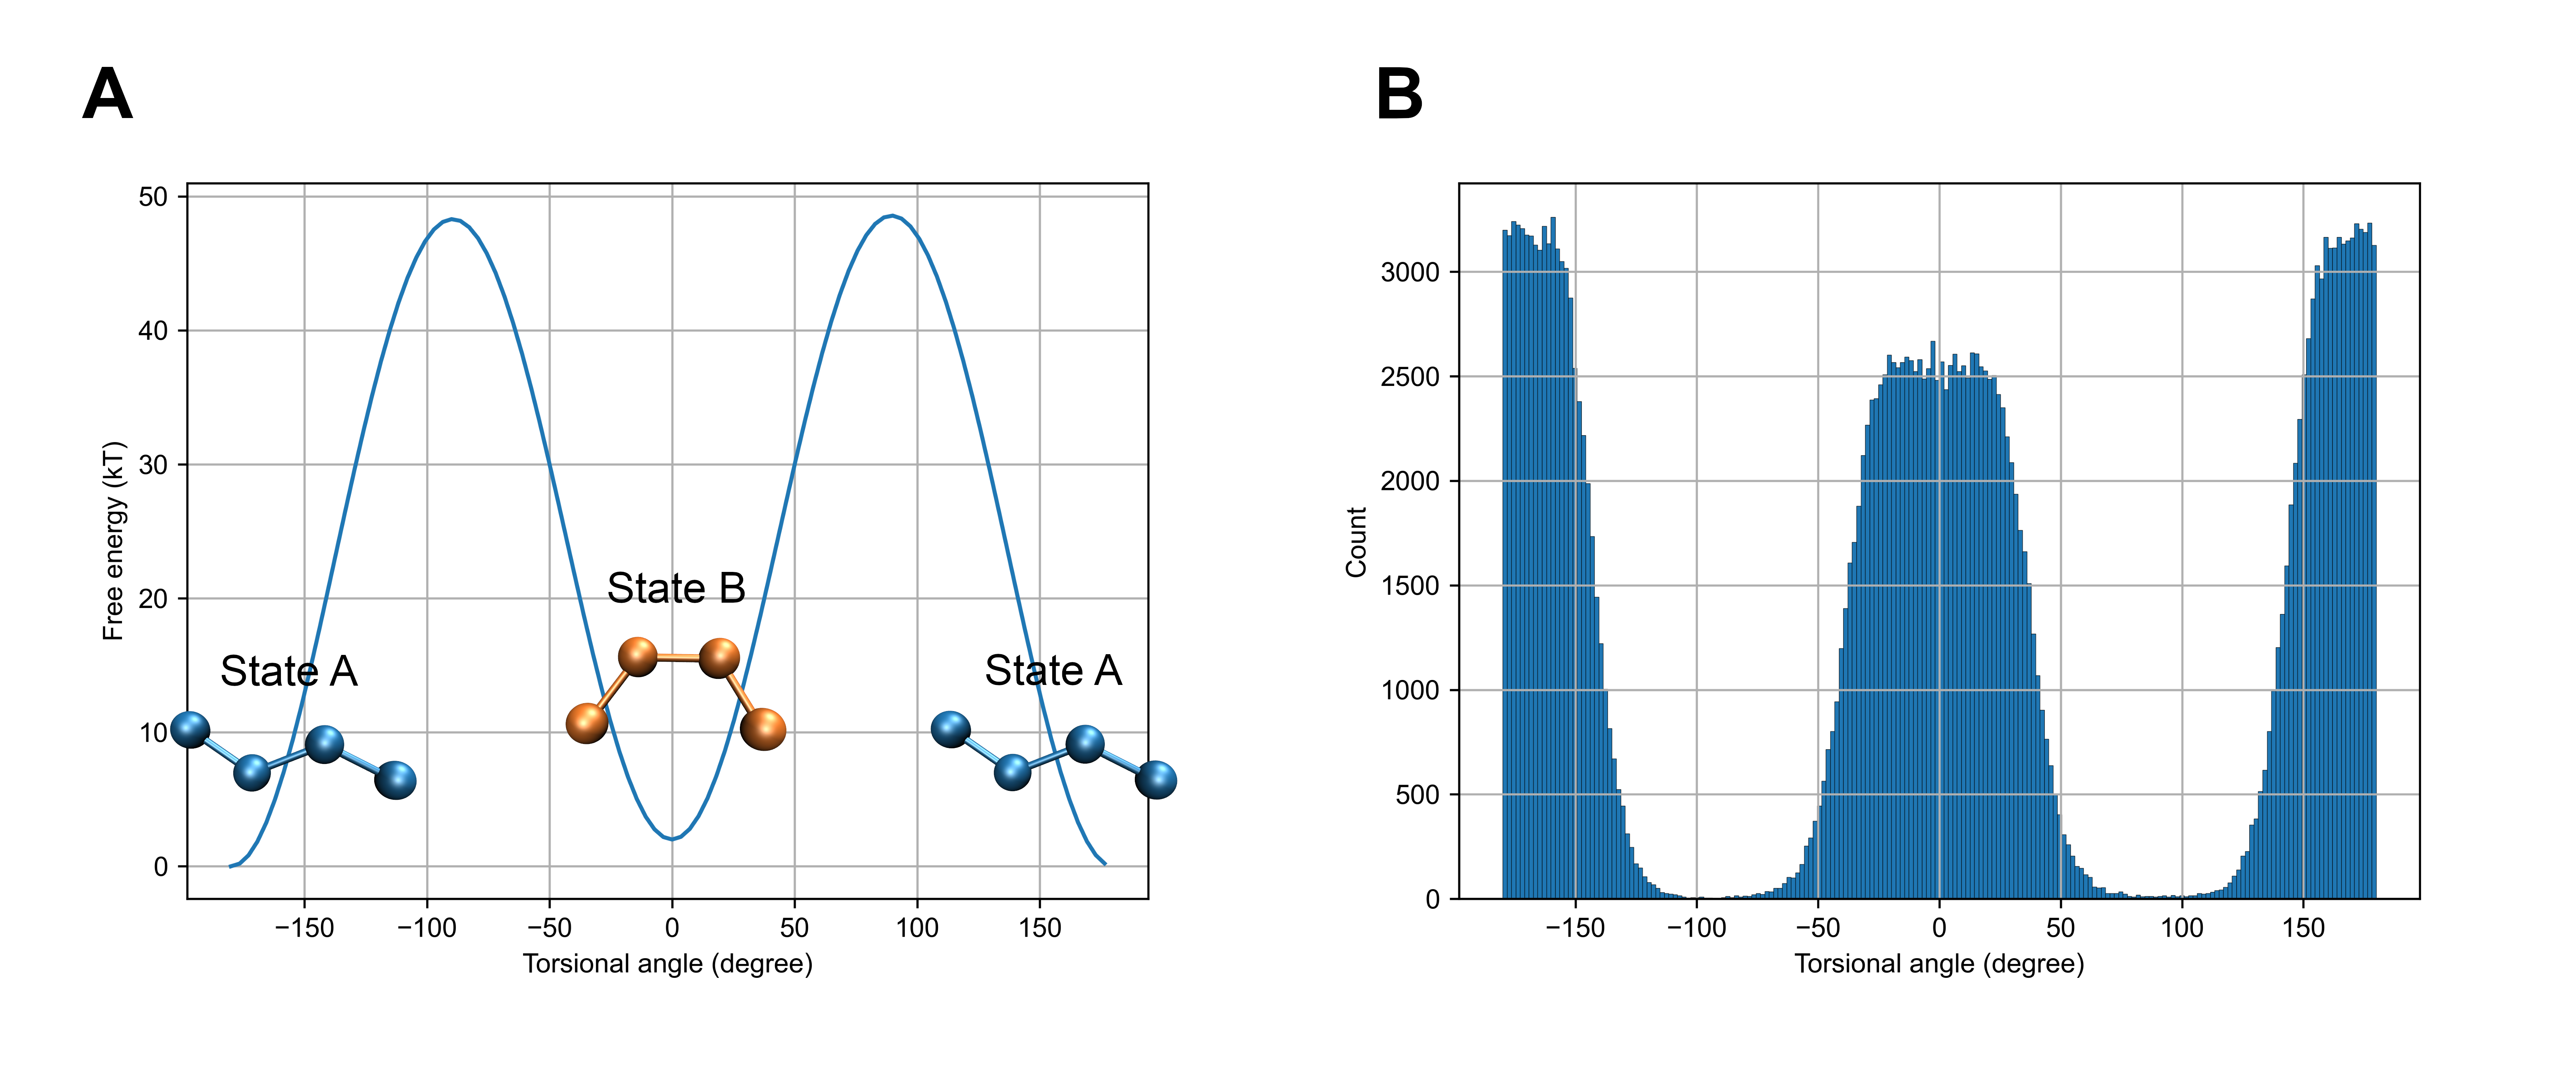
\includegraphics[width=\textwidth]{Figures/sys2_torsional_MetaD_annotated.png}   
    \caption{(A) The free energy profile as a function of the torsional angle. We refer the structures have a torsional angle of $\pm$180$^{\circ}$ and 0$^{\circ}$ as State A (trans isomer) and State B (cis isomer). The torsional free energy barrier starting from either state is around 48.56 kT, which might not be exact since the analysis was done on a very short (5 ns) simulation solely for generating configurations at both states. (B) The histogram of the sampled torsional angle in the torsional metadynamics. As can be seen, the system was able to sample both states frequently during the short simulation.}
    \label{sys2_torsional_MetaD}
\end{figure}

\renewcommand{\thefigure}{S\arabic{figure}}
\begin{figure}[H]
    \centering
    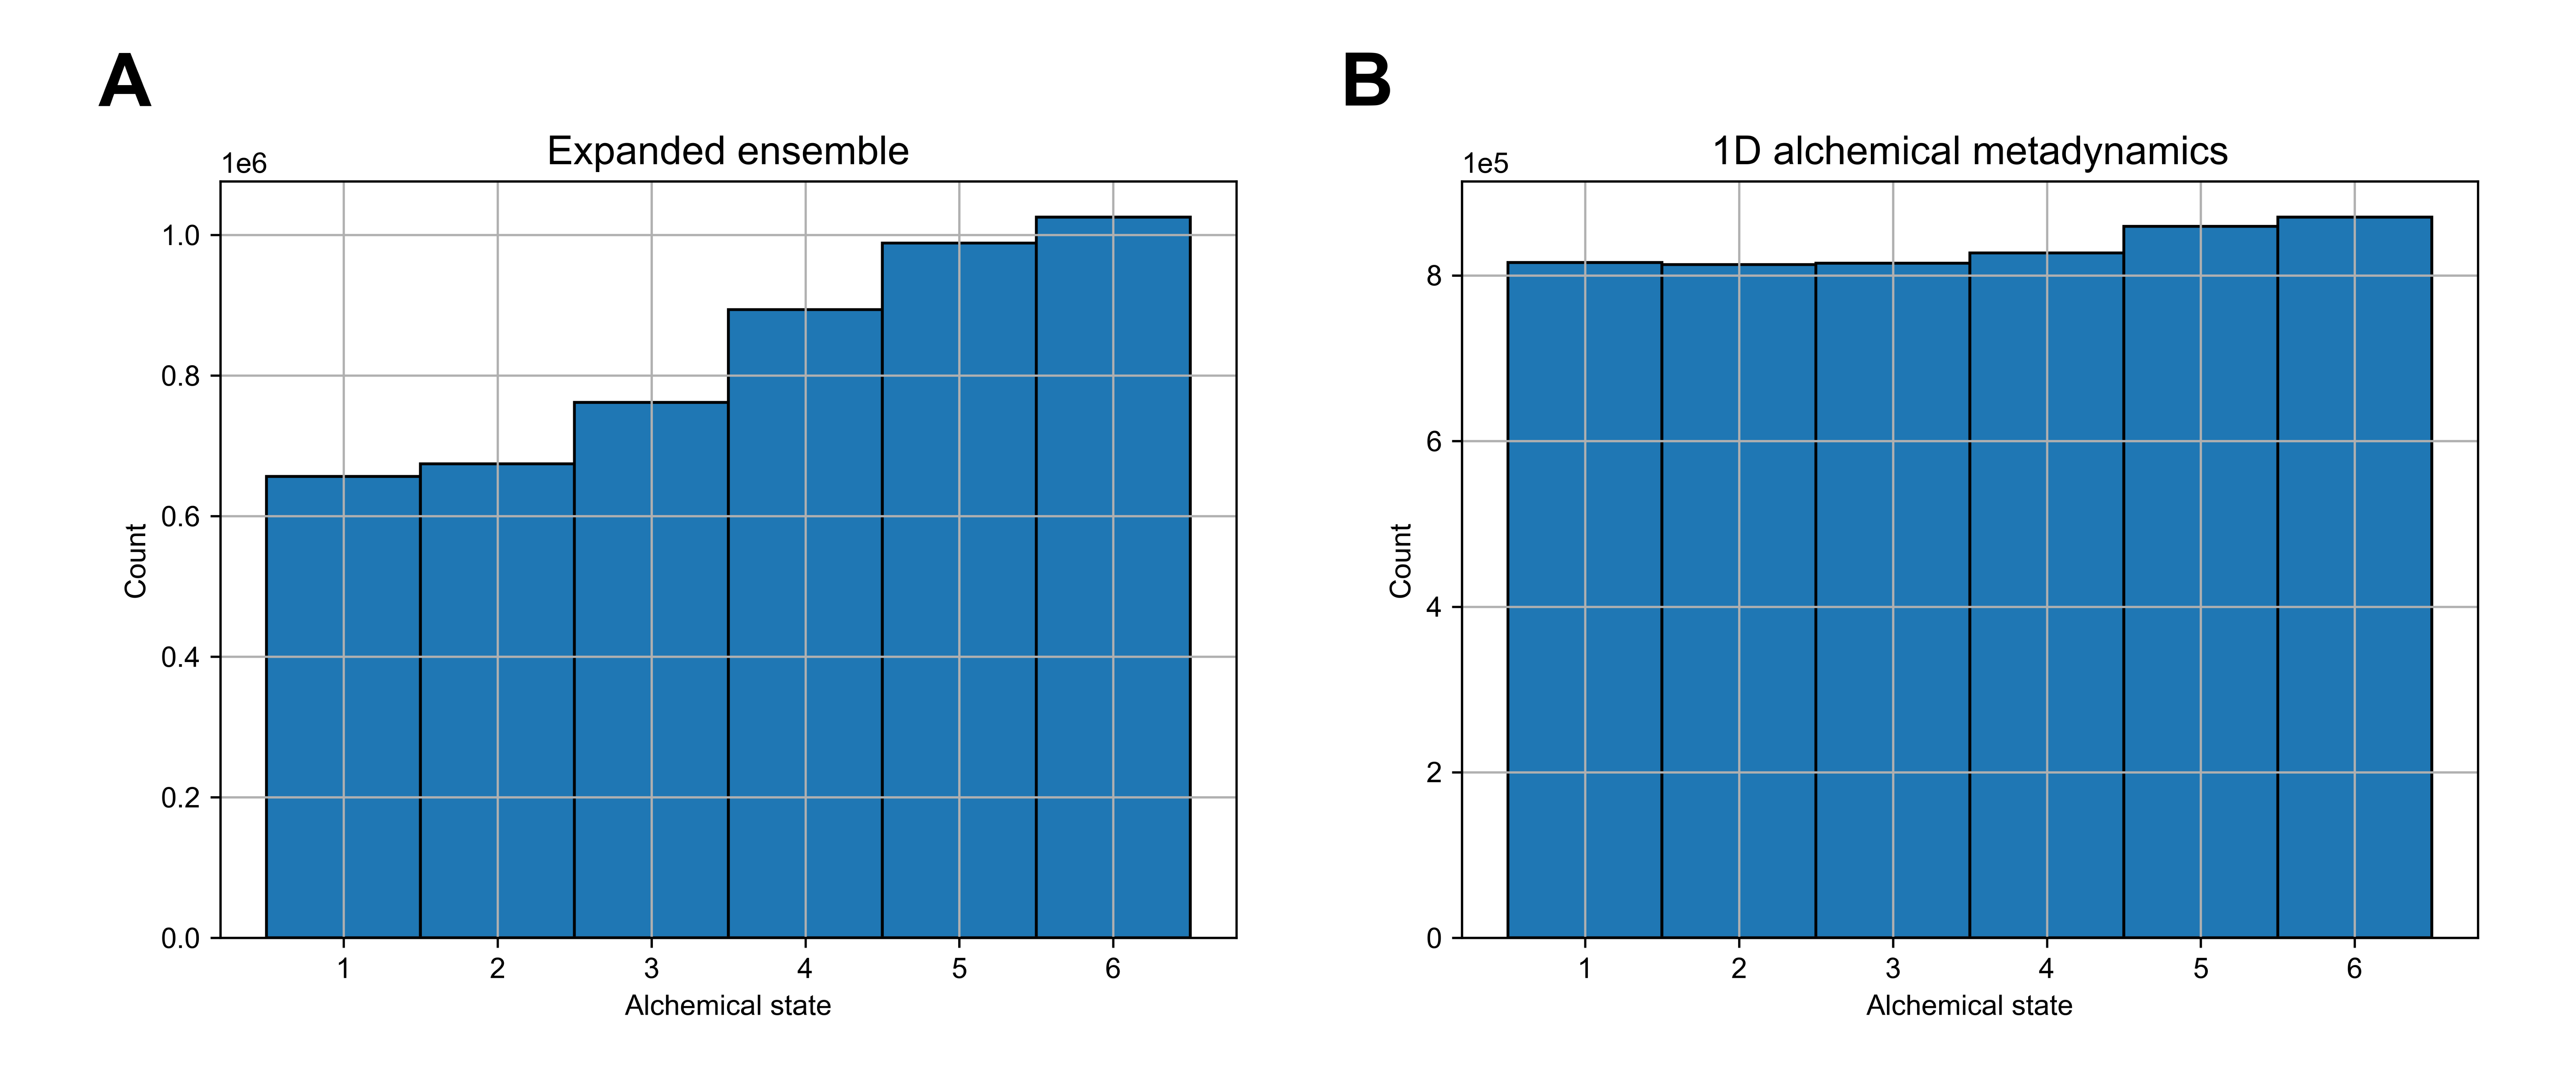
\includegraphics[width=\textwidth]{Figures/sys1_histograms.png}   
    \caption{The histograms of the state visitation in (A) expanded ensemble and (B) 1D alchemical metadynamics of System 1. Both simulations were able to sample all the intermediate states frequently.}
    \label{sys1_hist}
\end{figure}

\renewcommand{\thefigure}{S\arabic{figure}}
\begin{figure}[H]
    \centering
    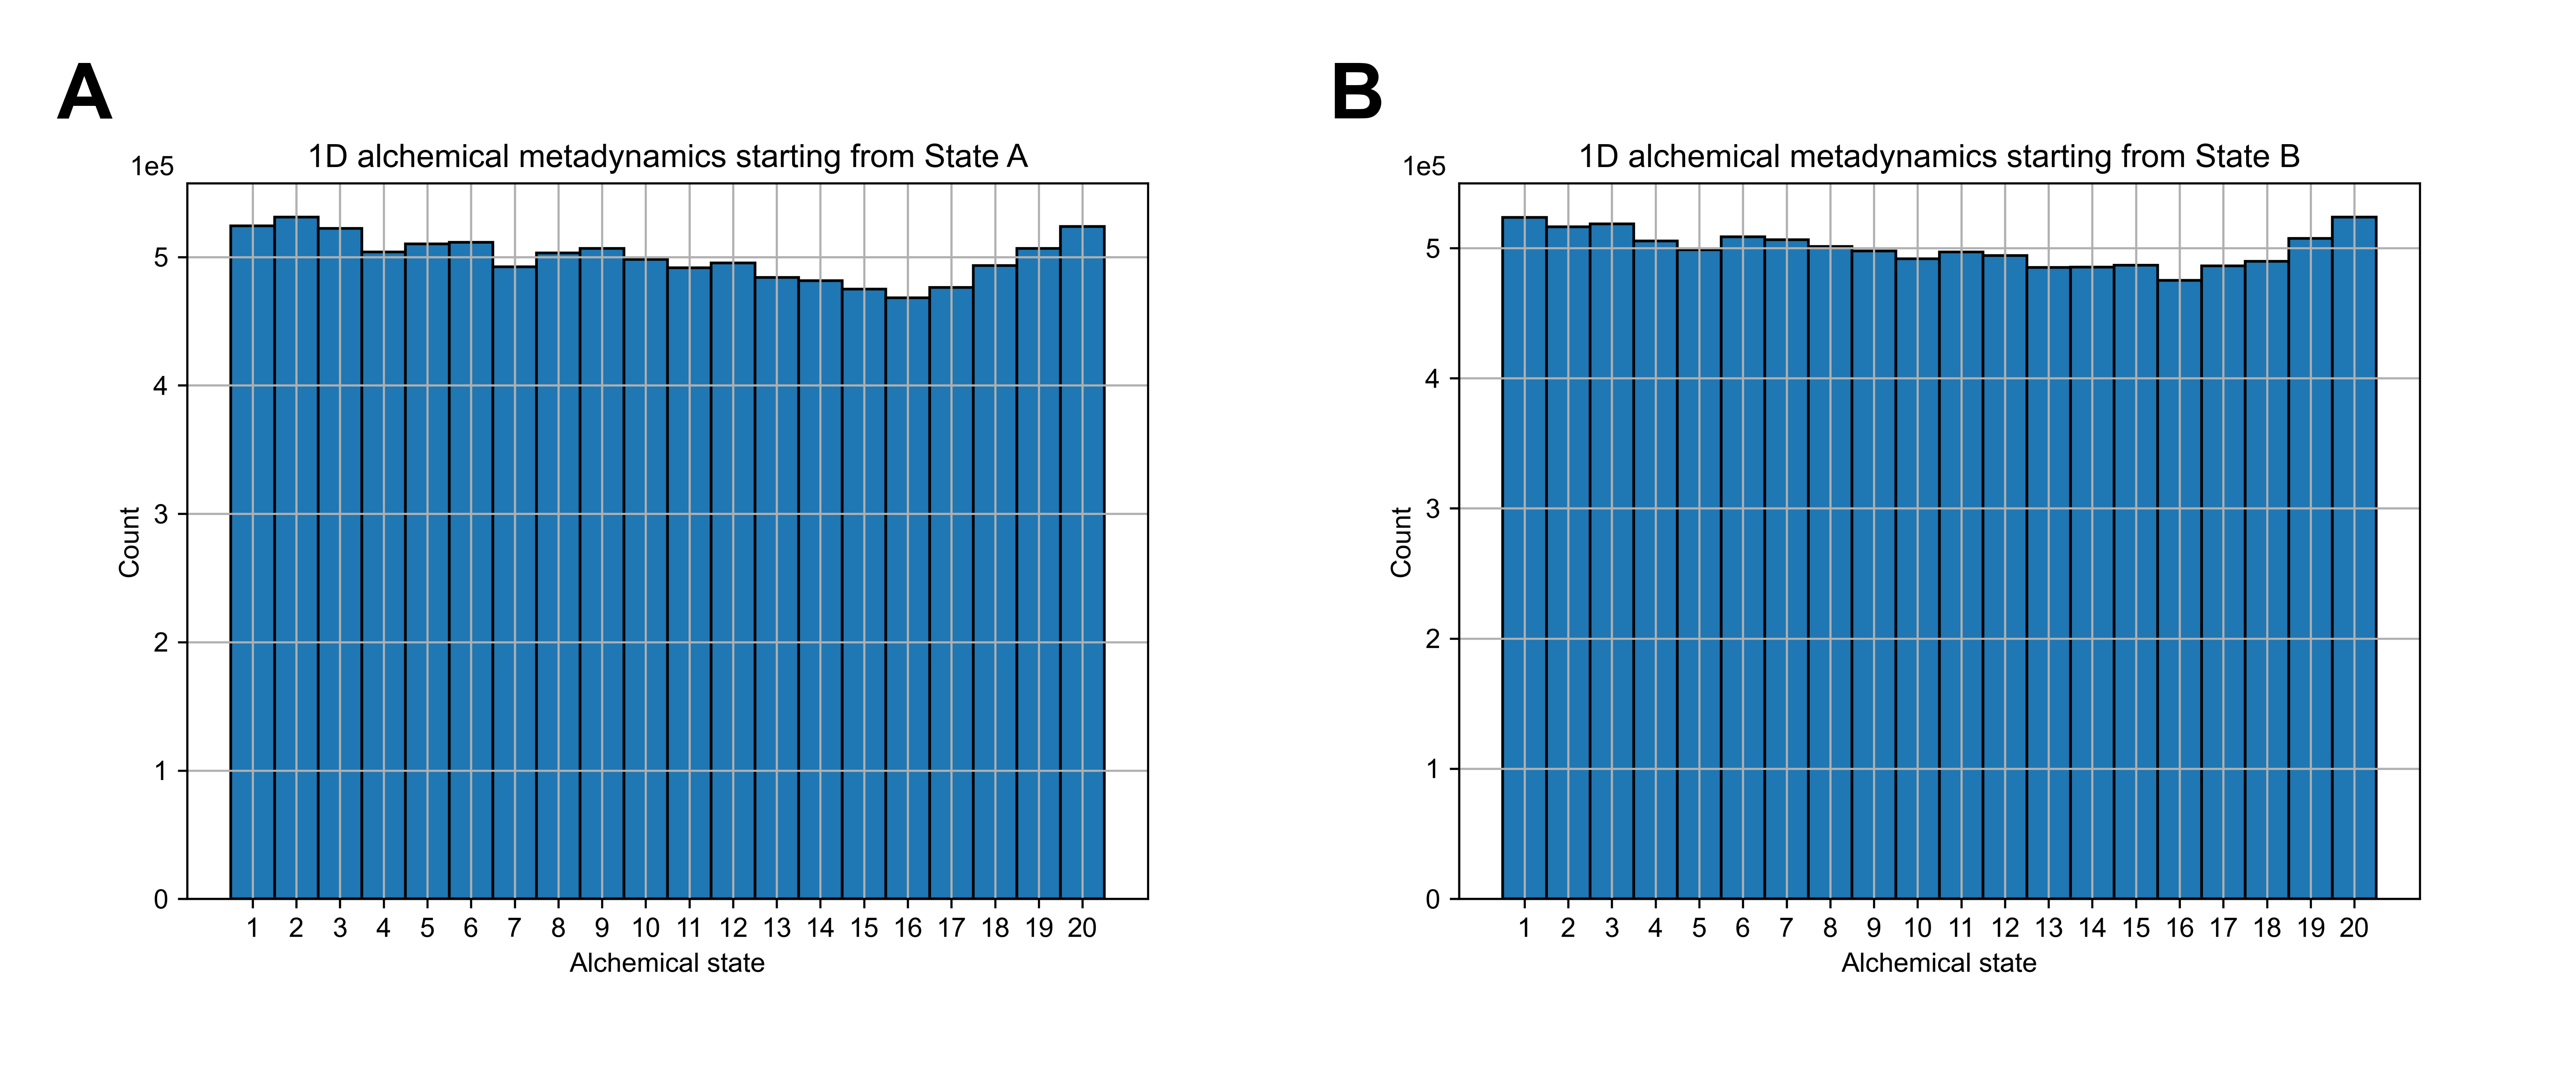
\includegraphics[width=\textwidth]{Figures/1D_lambda_hist.png}   
    \caption{The histograms of the state visitation in the 1D alchemical metadynamics starting from (A) State A and (B) State B. Both simulations were able to freely sample the alchemical space.}
    \label{sys2_1D_hist}
\end{figure}

\renewcommand{\thefigure}{S\arabic{figure}}
\begin{figure}[H]
    \centering
    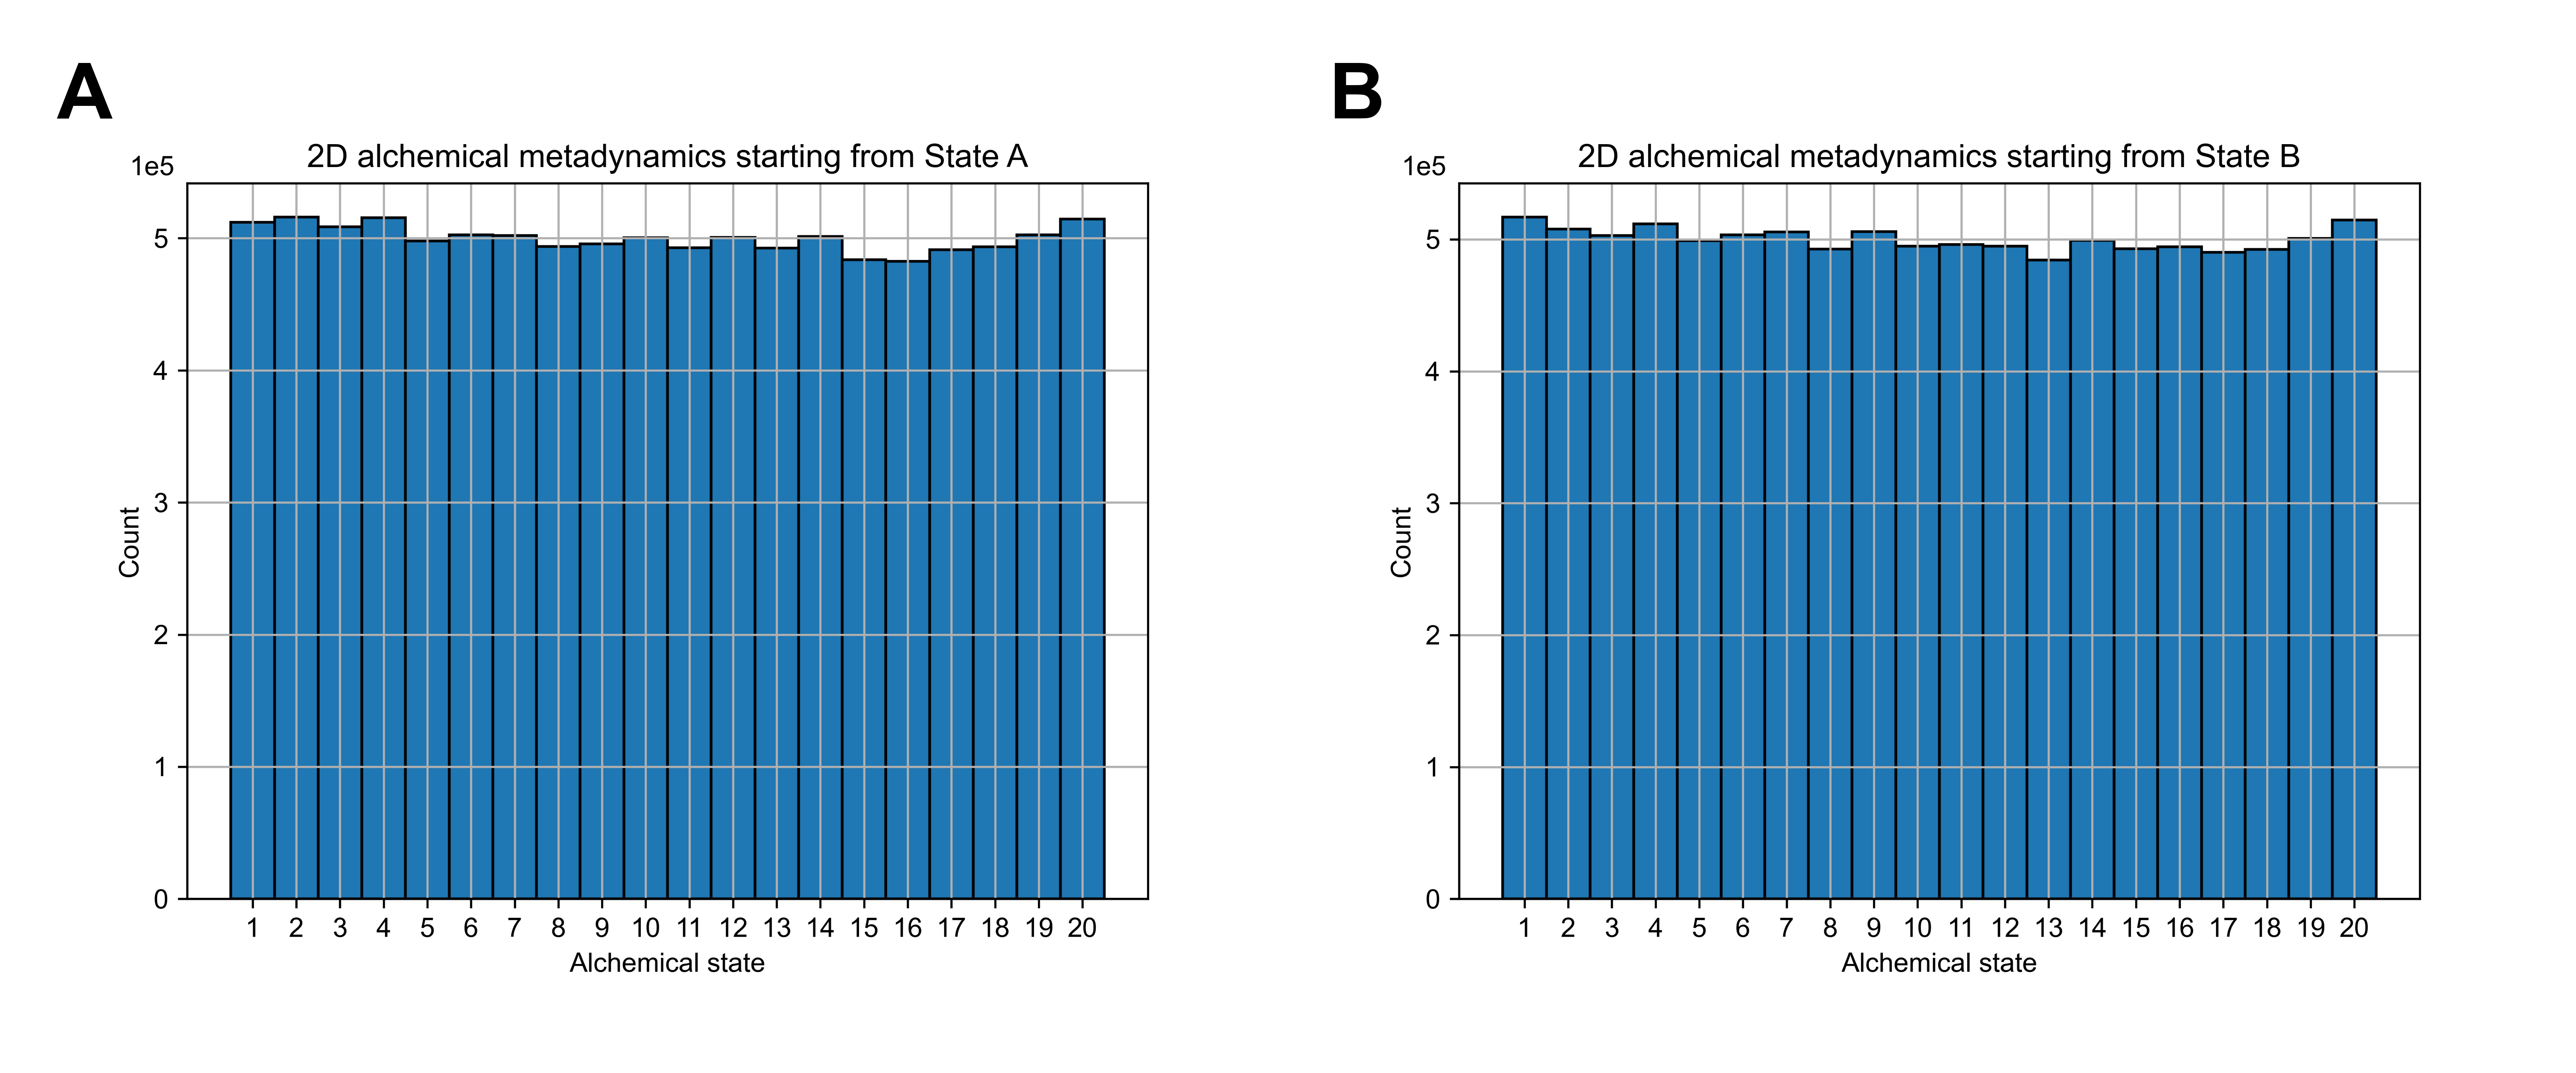
\includegraphics[width=\textwidth]{Figures/2D_lambda_hist.png}   
    \caption{The histograms of the state visitation in the 2D alchemical metadynamics starting from (A) State A and (B) State B. Similar to the two 1D simulations of System 2, both 2D simulations were able to freely sample the alchemical space.}
    \label{sys2_2D_hist}
\end{figure}

\renewcommand{\thefigure}{S\arabic{figure}}
\begin{figure}[H]
    \centering
    \includegraphics[width=\textwidth]{Figures/m6A_sampling.jpg}   
    \caption{(A) Value of the torsional angle N1-C6-N6-C10 as a function of time when the same torsional is used as CV, in a simulation performed at dynamic bias potential. In the 160 ns of simulations, the system only switches once from syn to anti state after about 8 ns and then back to syn after about 60 ns (B) Value of the torsional angle N1-C6-N6-C10 as a function of time when an averaged torsion between  N1-C6-N6-C10,  N1-C6-N6-H62, and  N1-C6-N6-H61 ($+ \pi$) is used as biasing collective variable. In this case, the system becomes diffusive on  N1-C6-N6-C10 after a few ns (C)  N1-C6-N6-C10 vs  N1-C6-N6-H62 when  N1-C6-N6-C10 is used as CV (D) N1-C6-N6-C10 vs  N1-C6-N6-H62 when the averaged torsion is used as CV. The three torsions mentioned here are coupled by an improper torsion that maintains the group C10, N6, H61, and H62 planar. The results shown here demonstrate that the improper torsion is not sufficiently stiff to maintain the consistency between the three torsions when enforcing the barrier crossing. As a consequence, the single N1-C6-N6-C10 torsion is not an optimal CV to allow a proper sampling of the torsional space.}
    \label{sampling}
\end{figure}


\clearpage
%\bibliography{refs}
\documentclass[journal=jacsat,manuscript=article]{achemso}

%%%%%%%%%%%%%%%%%%%%%%%%%%%%%%%%%%%%%%%%%%%%%%%%%%%%%%%%%%%%%%%%%%%%%
%% Place any additional packages needed here.  Only include packages
%% which are essential, to avoid problems later. Do NOT use any
%% packages which require e-TeX (for example etoolbox): the e-TeX
%% extensions are not currently available on the ACS conversion
%% servers.
%%%%%%%%%%%%%%%%%%%%%%%%%%%%%%%%%%%%%%%%%%%%%%%%%%%%%%%%%%%%%%%%%%%%%
\usepackage[version=3]{mhchem} % Formula subscripts using \ce{}

%%%%%%%%%%%%%%%%%%%%%%%%%%%%%%%%%%%%%%%%%%%%%%%%%%%%%%%%%%%%%%%%%%%%%
%% If issues arise when submitting your manuscript, you may want to
%% un-comment the next line.  This provides information on the
%% version of every file you have used.
%%%%%%%%%%%%%%%%%%%%%%%%%%%%%%%%%%%%%%%%%%%%%%%%%%%%%%%%%%%%%%%%%%%%%
%%\listfiles

%%%%%%%%%%%%%%%%%%%%%%%%%%%%%%%%%%%%%%%%%%%%%%%%%%%%%%%%%%%%%%%%%%%%%
%% Place any additional macros here.  Please use \newcommand* where
%% possible, and avoid layout-changing macros (which are not used
%% when typesetting).
%%%%%%%%%%%%%%%%%%%%%%%%%%%%%%%%%%%%%%%%%%%%%%%%%%%%%%%%%%%%%%%%%%%%%
\newcommand*\mycommand[1]{\texttt{\emph{#1}}}
\newcommand{\bfv}[1]{{\mbox{\boldmath{$#1$}}}}
\newcommand{\x}{\bfv{x}}
\usepackage{xr}
\makeatletter
\newcommand*{\addFileDependency}[1]{% argument=file name and extension
  \typeout{(#1)}
  \@addtofilelist{#1}
  \IfFileExists{#1}{}{\typeout{No file #1.}}
}
\makeatother

\newcommand*{\myexternaldocument}[1]{%
    \externaldocument{#1}%
    \addFileDependency{#1.tex}%
    \addFileDependency{#1.aux}%
}

\myexternaldocument{main}
%%%%%%%%%%%%%%%%%%%%%%%%%%%%%%%%%%%%%%%%%%%%%%%%%%%%%%%%%%%%%%%%%%%%%
%% Meta-data block
%% ---------------
%% Each author should be given as a separate \author command.
%%
%% Corresponding authors should have an e-mail given after the author
%% name as an \email command. Phone and fax numbers can be given
%% using \phone and \fax, respectively; this information is optional.
%%
%% The affiliation of authors is given after the authors; each
%% \affiliation command applies to all preceding authors not already
%% assigned an affiliation.
%%
%% The affiliation takes an option argument for the short name.  This
%% will typically be something like "University of Somewhere".
%%
%% The \altaffiliation macro should be used for new address, etc.
%% On the other hand, \alsoaffiliation is used on a per author basis
%% when authors are associated with multiple institutions.
%%%%%%%%%%%%%%%%%%%%%%%%%%%%%%%%%%%%%%%%%%%%%%%%%%%%%%%%%%%%%%%%%%%%%
\author{Wei-Tse Hsu}
\affiliation{Department of Chemical and Biological Engineering, University of Colorado Boulder, Boulder, CO 80305}
\author{Valerio Piomponi}
\affiliation{Scuola Internazionale Superiore di Studi Avanzati, Trieste, Italy}
\author{Pascal T. Merz}
\affiliation{Department of Chemical and Biological Engineering, University of Colorado Boulder, Boulder, CO 80305}
\author{Giovanni Bussi}
\affiliation{Scuola Internazionale Superiore di Studi Avanzati, Trieste, Italy}
\author{Michael R. Shirts}
\affiliation{Department of Chemical and Biological Engineering, University of Colorado Boulder, Boulder, CO 80305}
\email{michael.shirts@colorado.edu}

%%%%%%%%%%%%%%%%%%%%%%%%%%%%%%%%%%%%%%%%%%%%%%%%%%%%%%%%%%%%%%%%%%%%%
%% The document title should be given as usual. Some journals require
%% a running title from the author: this should be supplied as an
%% optional argument to \title.
%%%%%%%%%%%%%%%%%%%%%%%%%%%%%%%%%%%%%%%%%%%%%%%%%%%%%%%%%%%%%%%%%%%%%
\title
  {Supporting Information: Adding alchemical variables to metadynamics to enhance sampling in free energy calculations}

%%%%%%%%%%%%%%%%%%%%%%%%%%%%%%%%%%%%%%%%%%%%%%%%%%%%%%%%%%%%%%%%%%%%%
%% Some journals require a list of abbreviations or keywords to be
%% supplied. These should be set up here, and will be printed after
%% the title and author information, if needed.
%%%%%%%%%%%%%%%%%%%%%%%%%%%%%%%%%%%%%%%%%%%%%%%%%%%%%%%%%%%%%%%%%%%%%
% \abbreviations{IR,NMR,UV}
%\keywords{American Chemical Society, \LaTeX}

%%%%%%%%%%%%%%%%%%%%%%%%%%%%%%%%%%%%%%%%%%%%%%%%%%%%%%%%%%%%%%%%%%%%%
%% The manuscript does not need to include \maketitle, which is
%% executed automatically.
%%%%%%%%%%%%%%%%%%%%%%%%%%%%%%%%%%%%%%%%%%%%%%%%%%%%%%%%%%%%%%%%%%%%%
\begin{document}

% \clearpage
\section{Comparison of methylation free energy calculations with dynamic and static biases}
% We should include the lengths of the simulations using the dynamic bias and mention the adopted truncation fraction, average fraction, number of blocks in block bootstrapping, number of iteration for each data point. We should also explain the meaning of the 4th point by explicitly stating what values the 4th point took the difference from. (Like what is done in the section of free energy calculations for the last system in the main text.) 
As a supplementary information, we show the free energy calculations with dynamic bias for the nucleotide and duplex systems. These calculations are done in comparison with the free energy differences computed with static bias presented in the main text. Specifically, simulations at dynamic bias were elongated up to 160 ns. For analysis, the first 60 ns were discarded, and the bias averaged over the remaining 100 ns was used to compute weights. Different numbers of blocks ranging 2 to 1000 were used to construct histograms in block boostrapping (200 iterations) and the largest uncertainty is reported. 

The figure below shows that with dynamic bias, the free energy estimates are more precise (lower statistical errors). This is mostly likely  attributable to the fact that the sampling in the CV space is more diffusive in these systems with dynamically updated weights. However, free energy estimates computed with dynamic bias are less accurate, i.e. the results differ more in alchemical metadynamics than in the case of Hamiltonian replica exchange (HREX). This is probably caused by the dynamic bias adding some small amount of history-dependent blurring. 

To further demonstrate the lower accuracy of the dynamic bias computation, the free energy difference ($\Delta G^{\text{dup, A}}_{syn/anti}$) between the two conformations of adenosine shown in Figure 3A in the main text is calculated. In the work by Piomponi et al.,~\cite{piomponi2022molecular} this value was assumed to be 0 because of the symmetry of the hydrogen atoms H61 and H62. Also, HREX used in the previous work does not have the access to the free energy landscape along the biased torsion, so the relative error is not given for the HREX case. In alchemical metadynamics, $\Delta G^{\text{dup, A}}_{anti/syn}$ was calculated as follows: 
\begin{equation}
    \Delta G^{\text{dup, A}}_{syn/anti}=-\frac{1}{\beta} \ln \left( \frac{\sum_{i \in anti} e^{\beta V^{\text{dup}}_{\text{tot}}(\eta_i, \lambda=0) }}{\sum_{i \in syn} e^{\beta V^{\text{dup}}_{\text{tot}}(\eta_i, \lambda=0)}}\right )
\end{equation} 

For most systems, the general understanding is that using plain metadynamics instead of doing the two-step procedure is better~\cite{bussi2020using}. It is likely the result is system dependent and related to the fact that even without a dynamic bias we can see many of transitions, thus a reasonable statistical error. In this way, we are clearly in the regime where fewer transitions at equilibrium are a safer estimate.

\renewcommand{\thefigure}{S\arabic{figure}}
\begin{figure}[H]
    \centering
    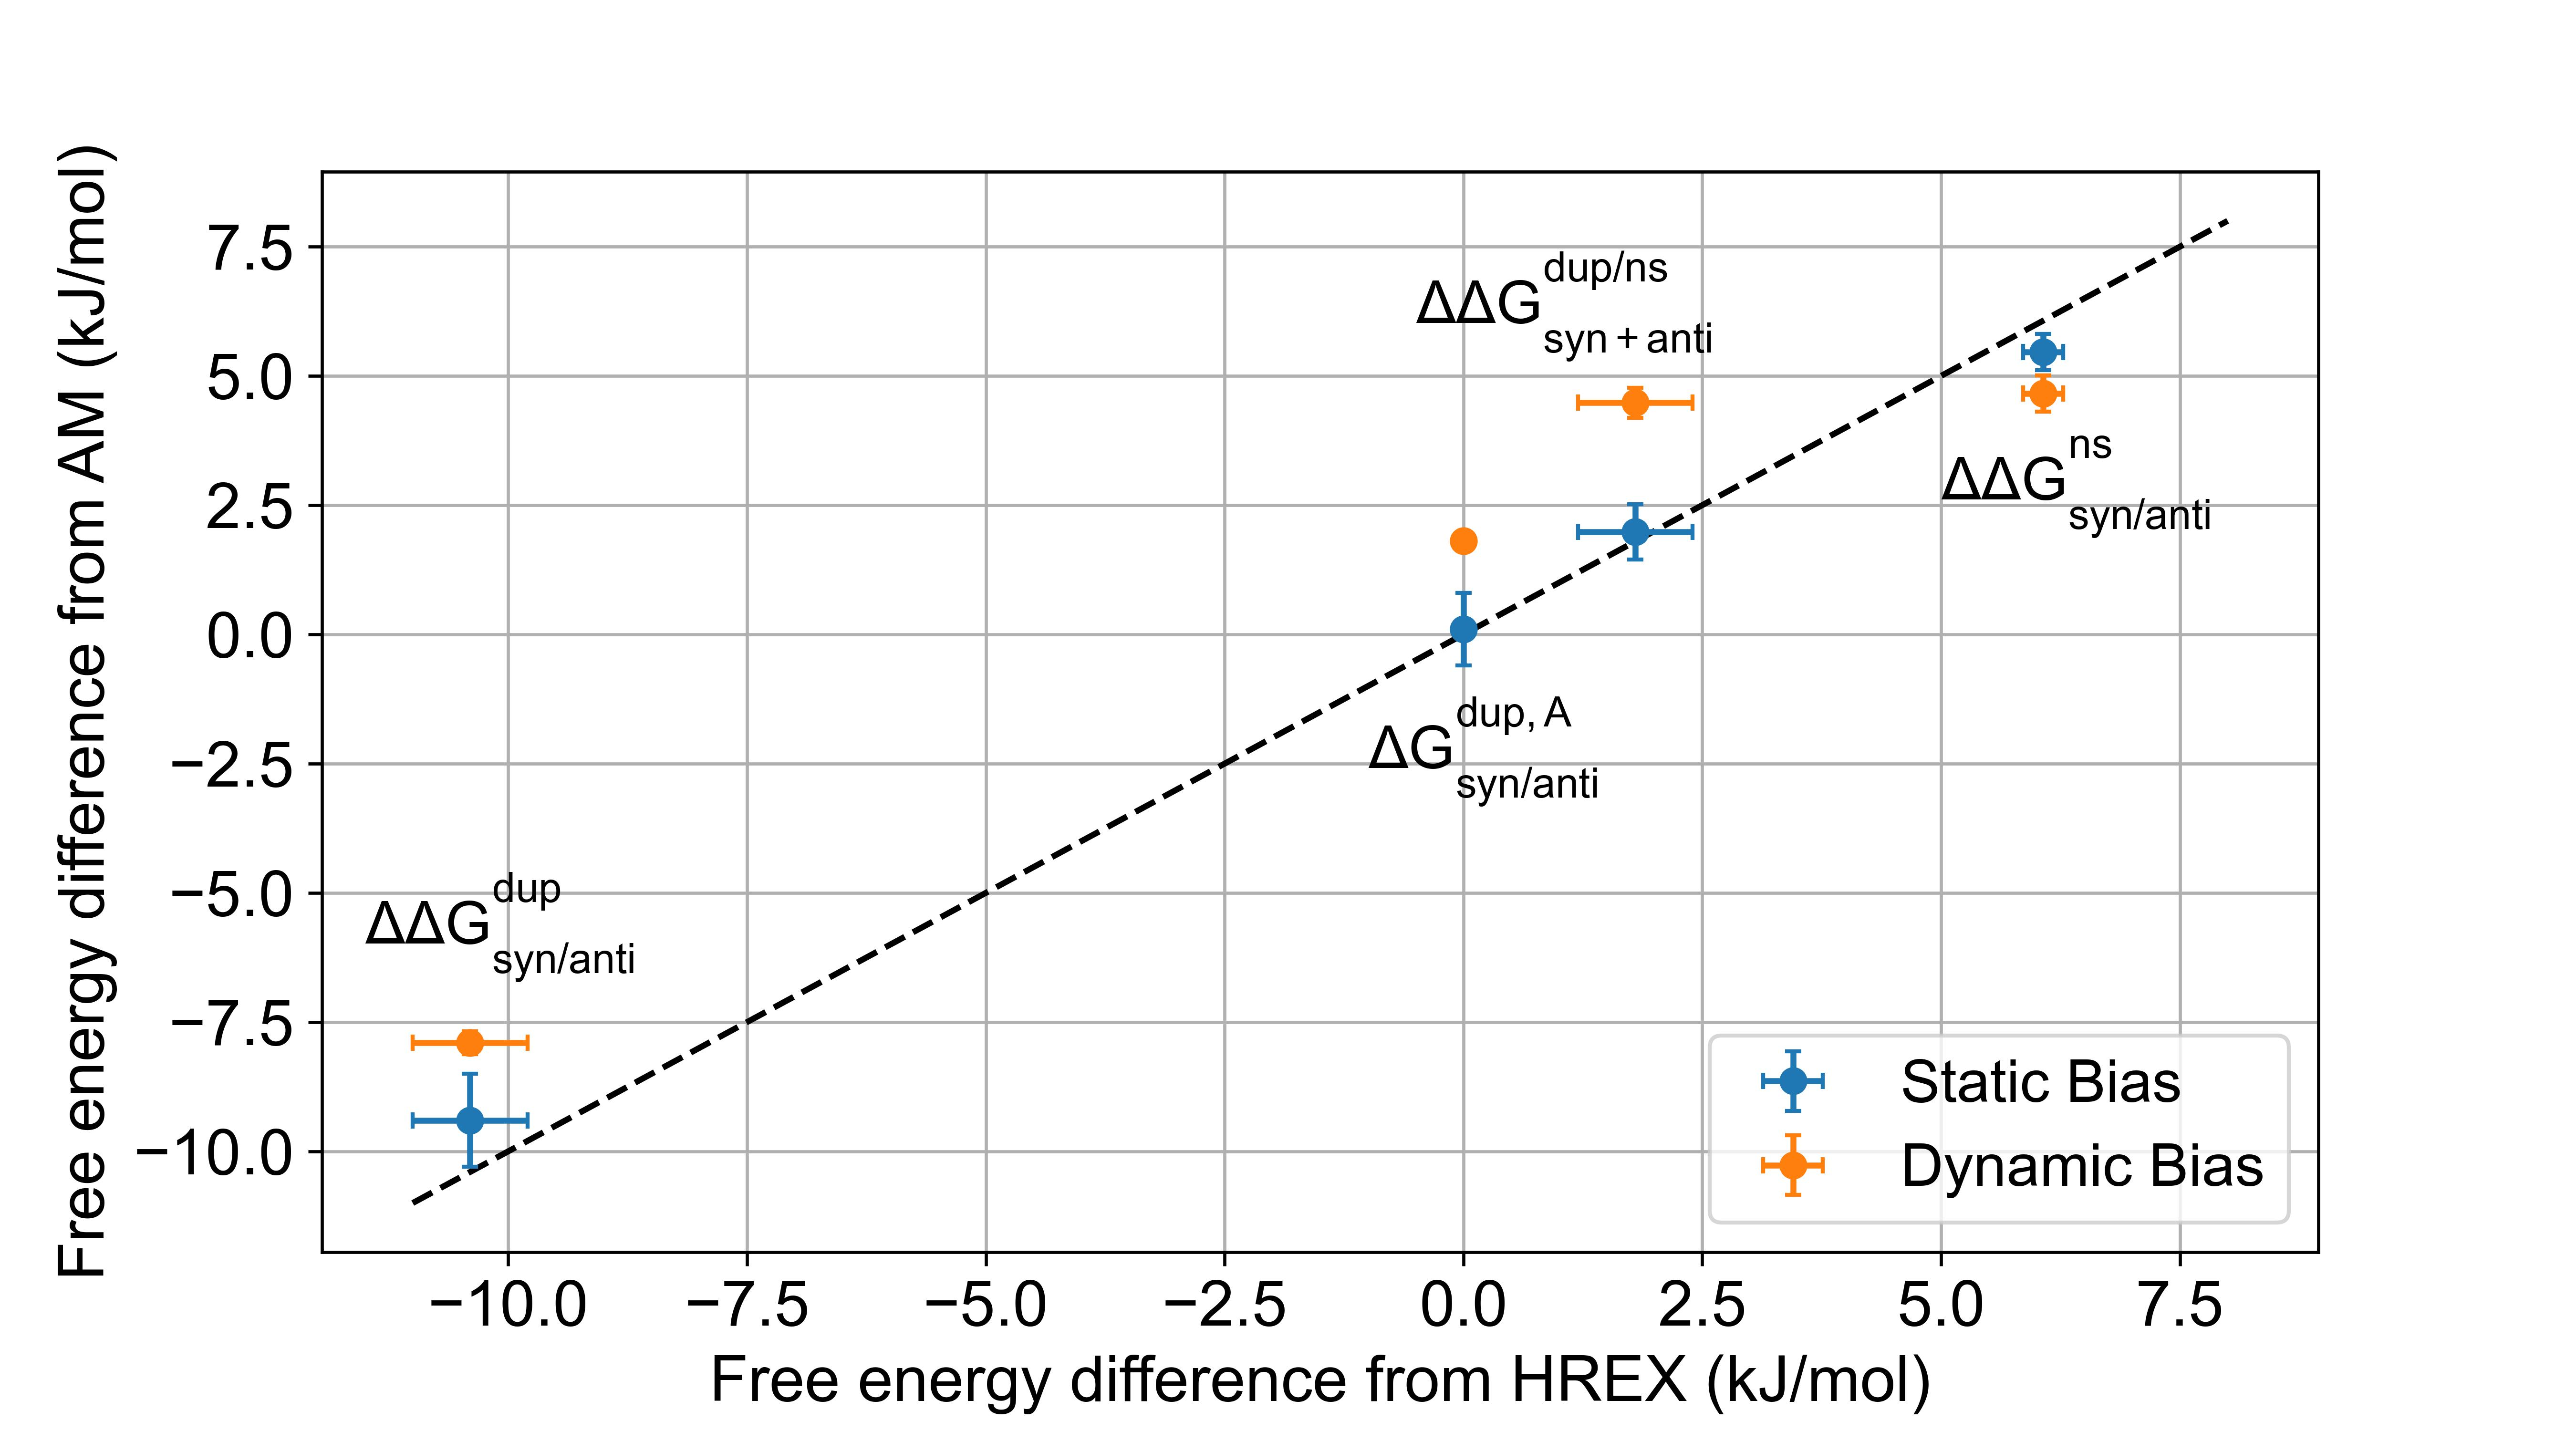
\includegraphics[width=\textwidth]{Figures/m6A_dynamic_static.jpg}   
    \caption{Comparison of free energy differences computed in Ref.~\cite{piomponi2022molecular} with Hamiltonian replica exchange (HREX) and $\Delta \Delta G$ computed with alchemical metadynamics (AM) in this work, for two cases: (1) static bias (as discussed in the main text) and (2) dynamic bias.}
    \label{compare_ACS}
\end{figure}

\section{Supplementary Figures}
\renewcommand{\thefigure}{S\arabic{figure}}
\begin{figure}[H]
    \centering
    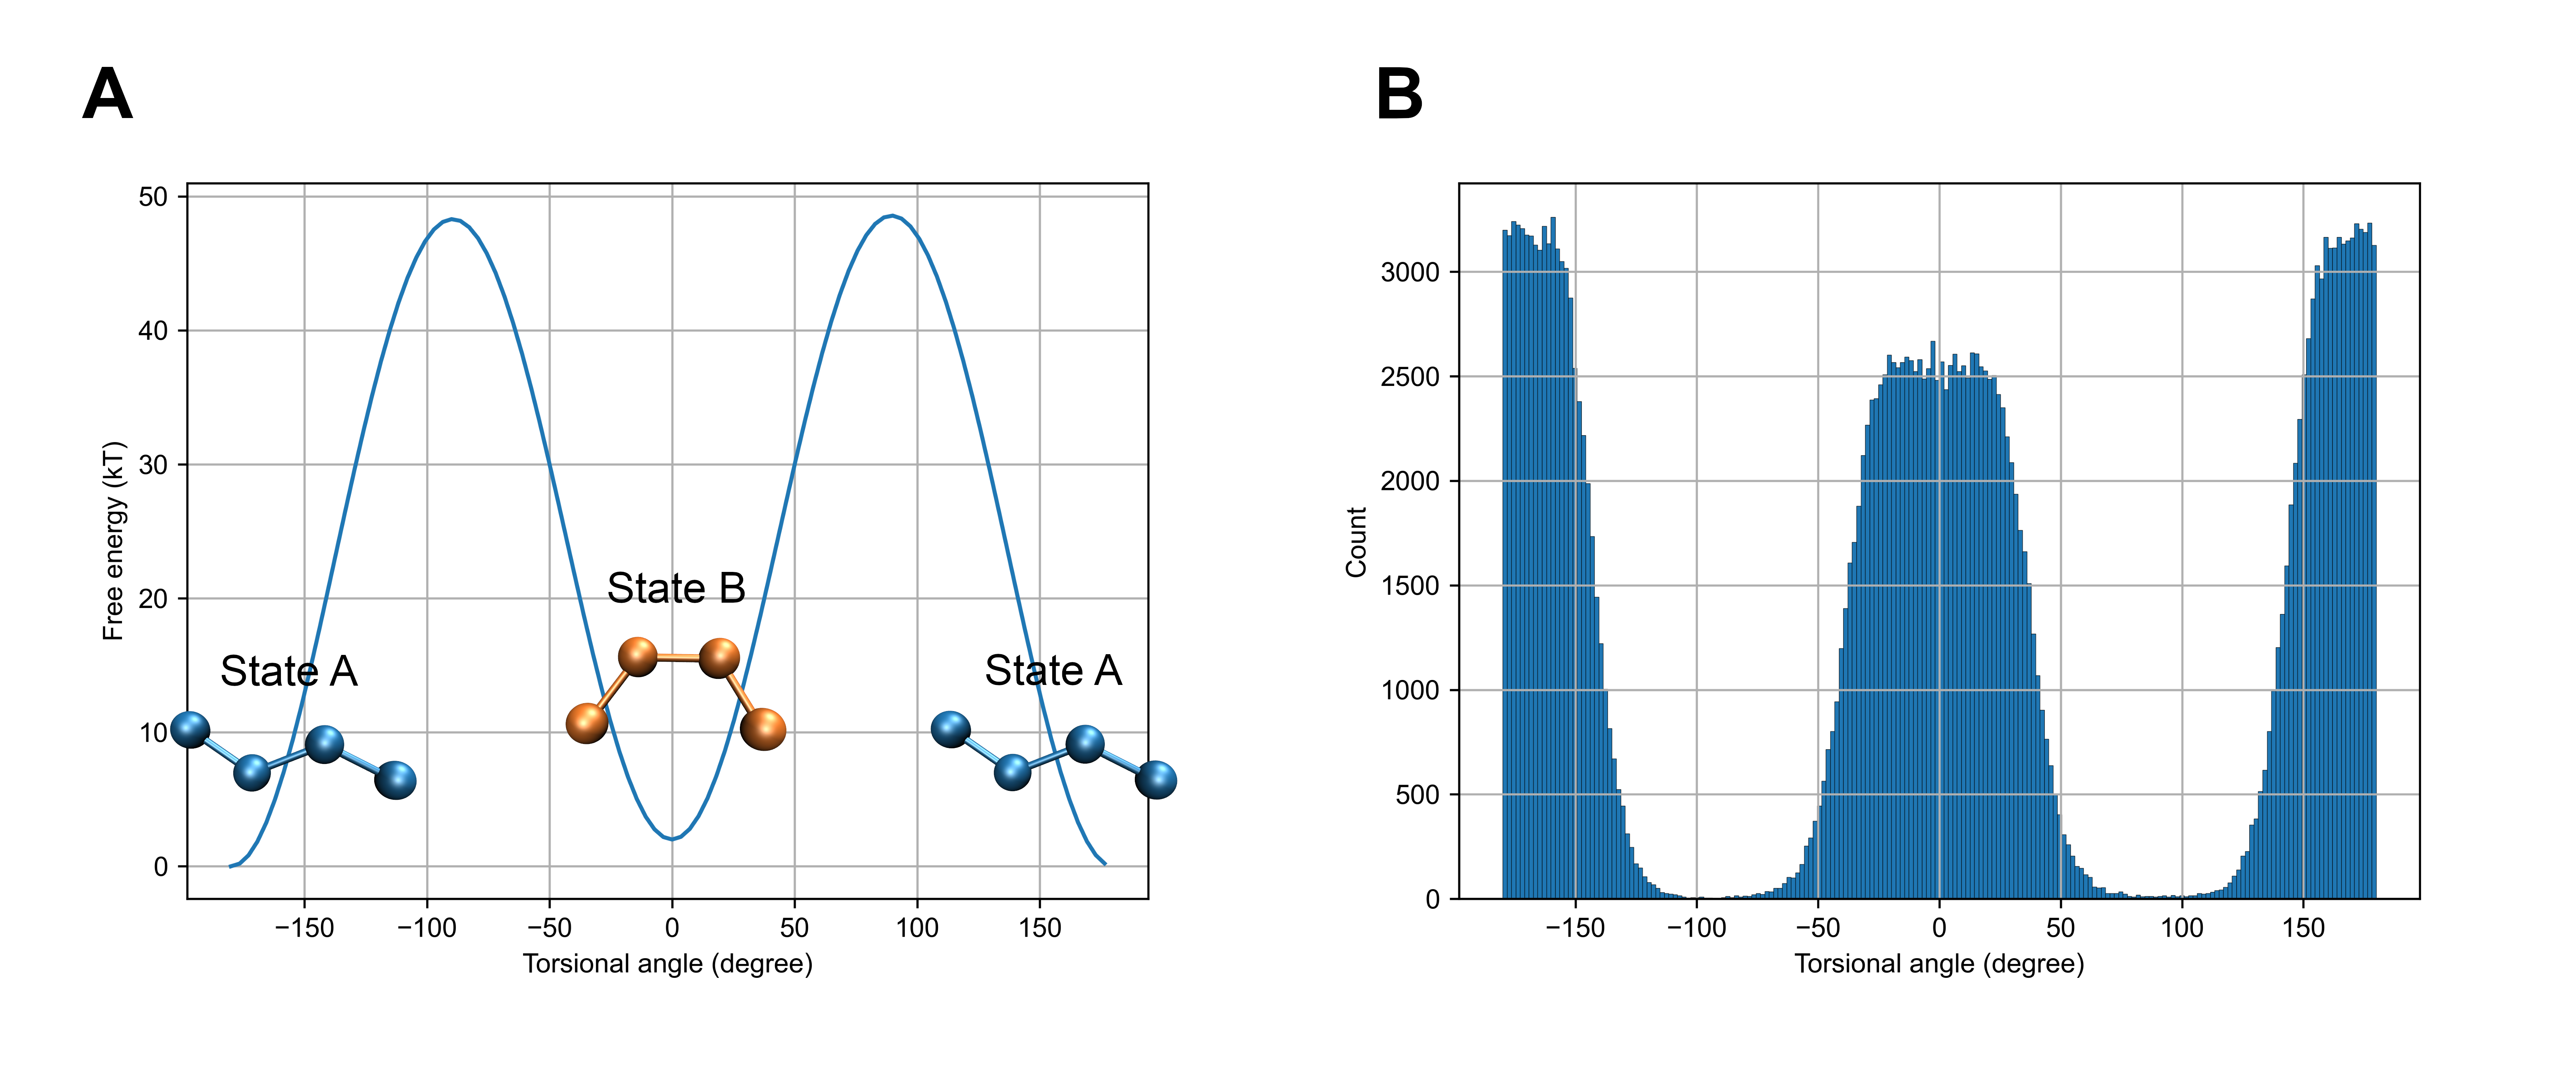
\includegraphics[width=\textwidth]{Figures/sys2_torsional_MetaD_annotated.png}   
    \caption{(A) The free energy profile as a function of the torsional angle. We refer the structures have a torsional angle of $\pm$180$^{\circ}$ and 0$^{\circ}$ as State A (trans isomer) and State B (cis isomer). The torsional free energy barrier starting from either state is around 48.56 kT, which might not be exact since the analysis was done on a very short (5 ns) simulation solely for generating configurations at both states. (B) The histogram of the sampled torsional angle in the torsional metadynamics. As can be seen, the system was able to sample both states frequently during the short simulation.}
    \label{sys2_torsional_MetaD}
\end{figure}

\renewcommand{\thefigure}{S\arabic{figure}}
\begin{figure}[H]
    \centering
    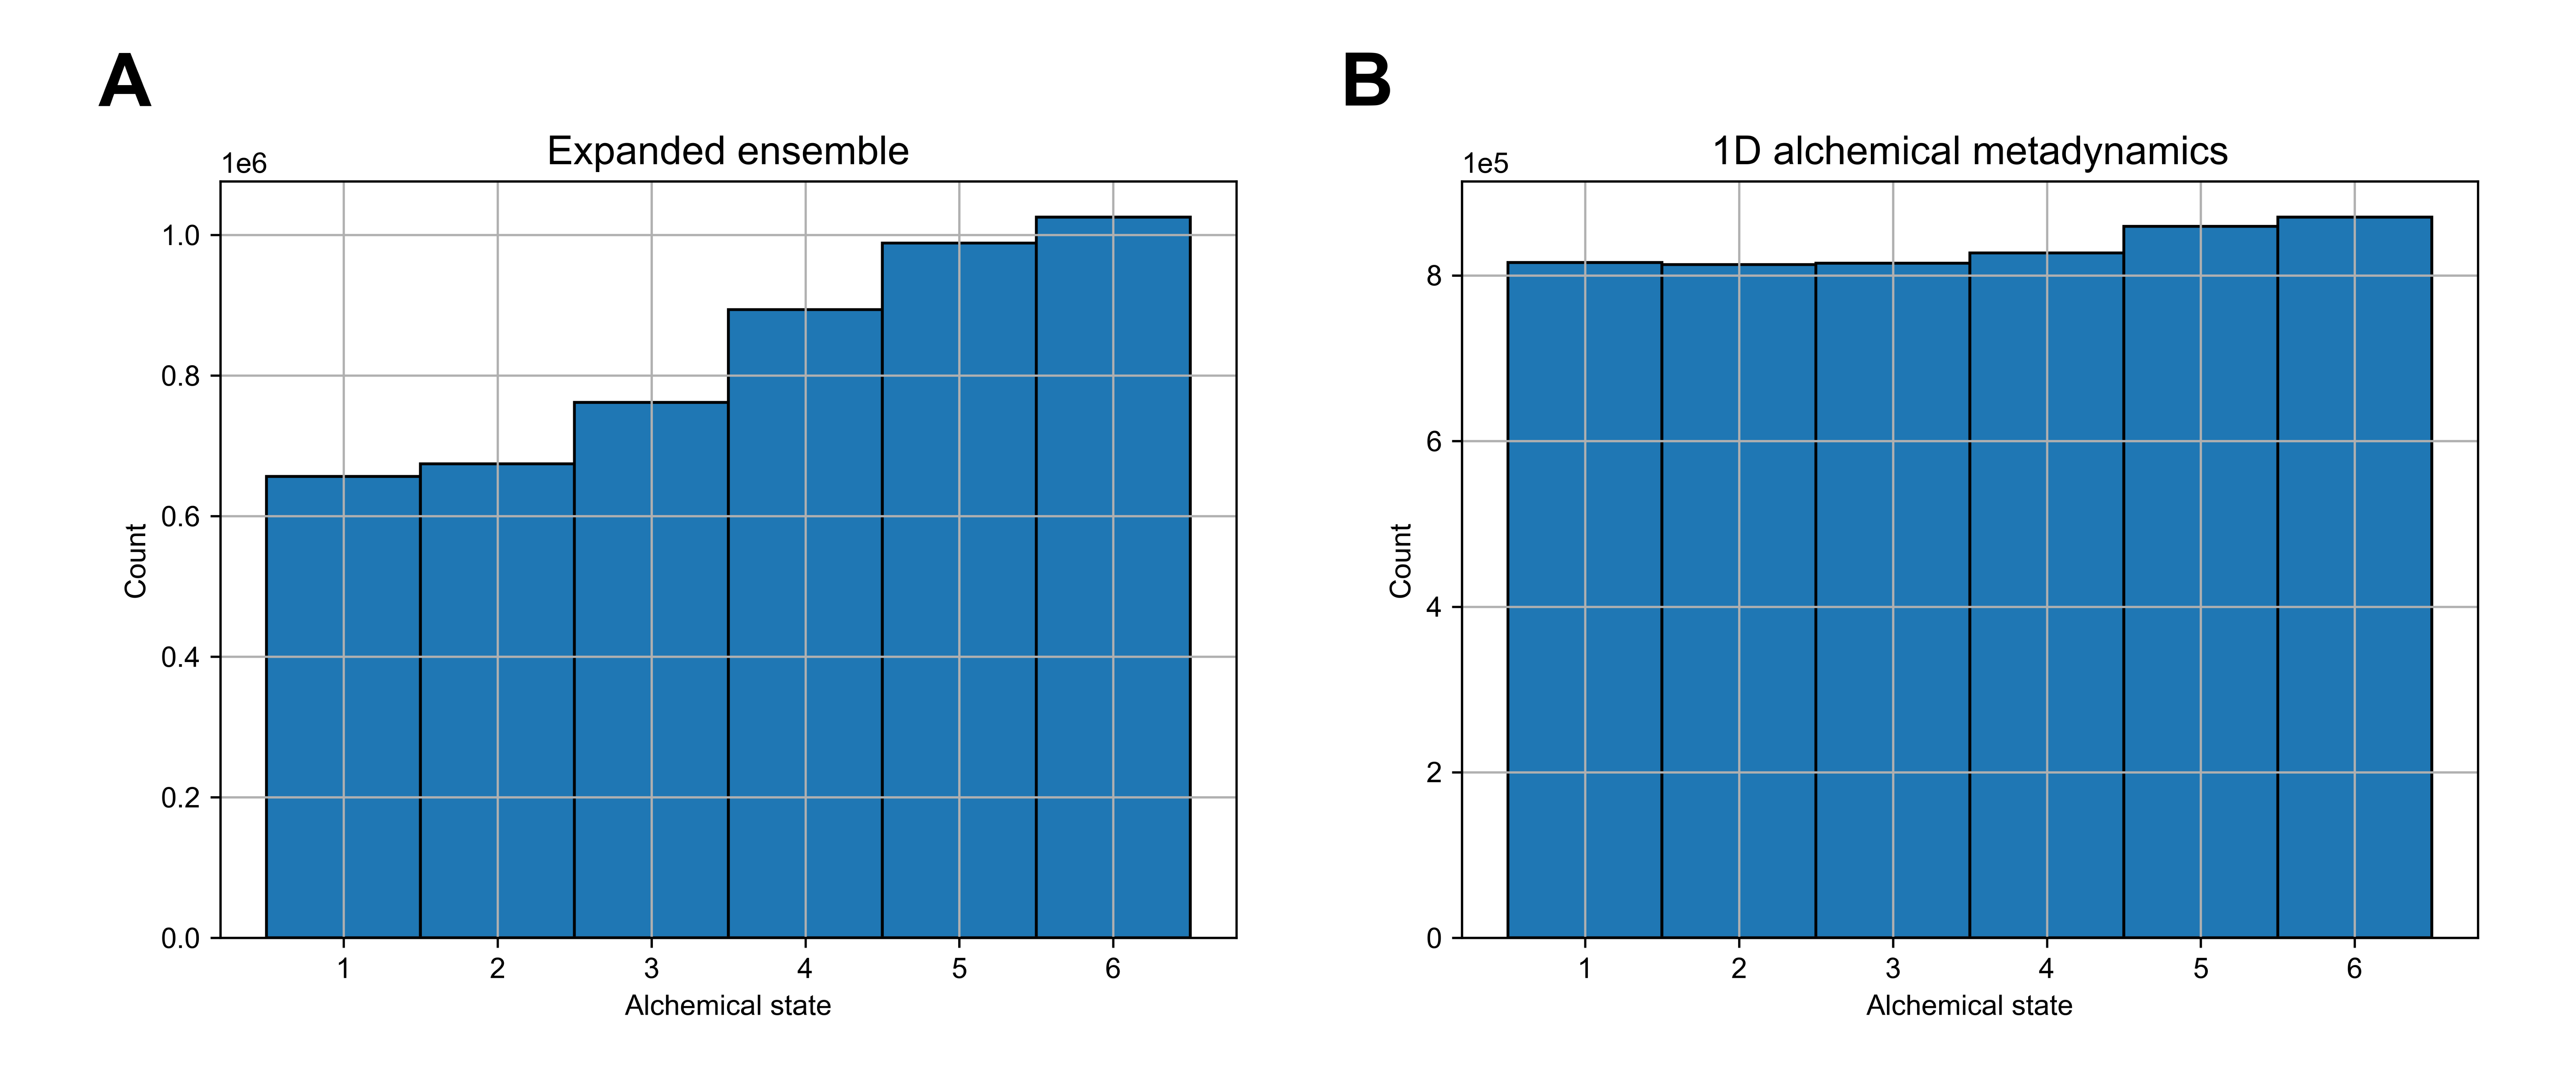
\includegraphics[width=\textwidth]{Figures/sys1_histograms.png}   
    \caption{The histograms of the state visitation in (A) expanded ensemble and (B) 1D alchemical metadynamics of System 1. Both simulations were able to sample all the intermediate states frequently.}
    \label{sys1_hist}
\end{figure}

\renewcommand{\thefigure}{S\arabic{figure}}
\begin{figure}[H]
    \centering
    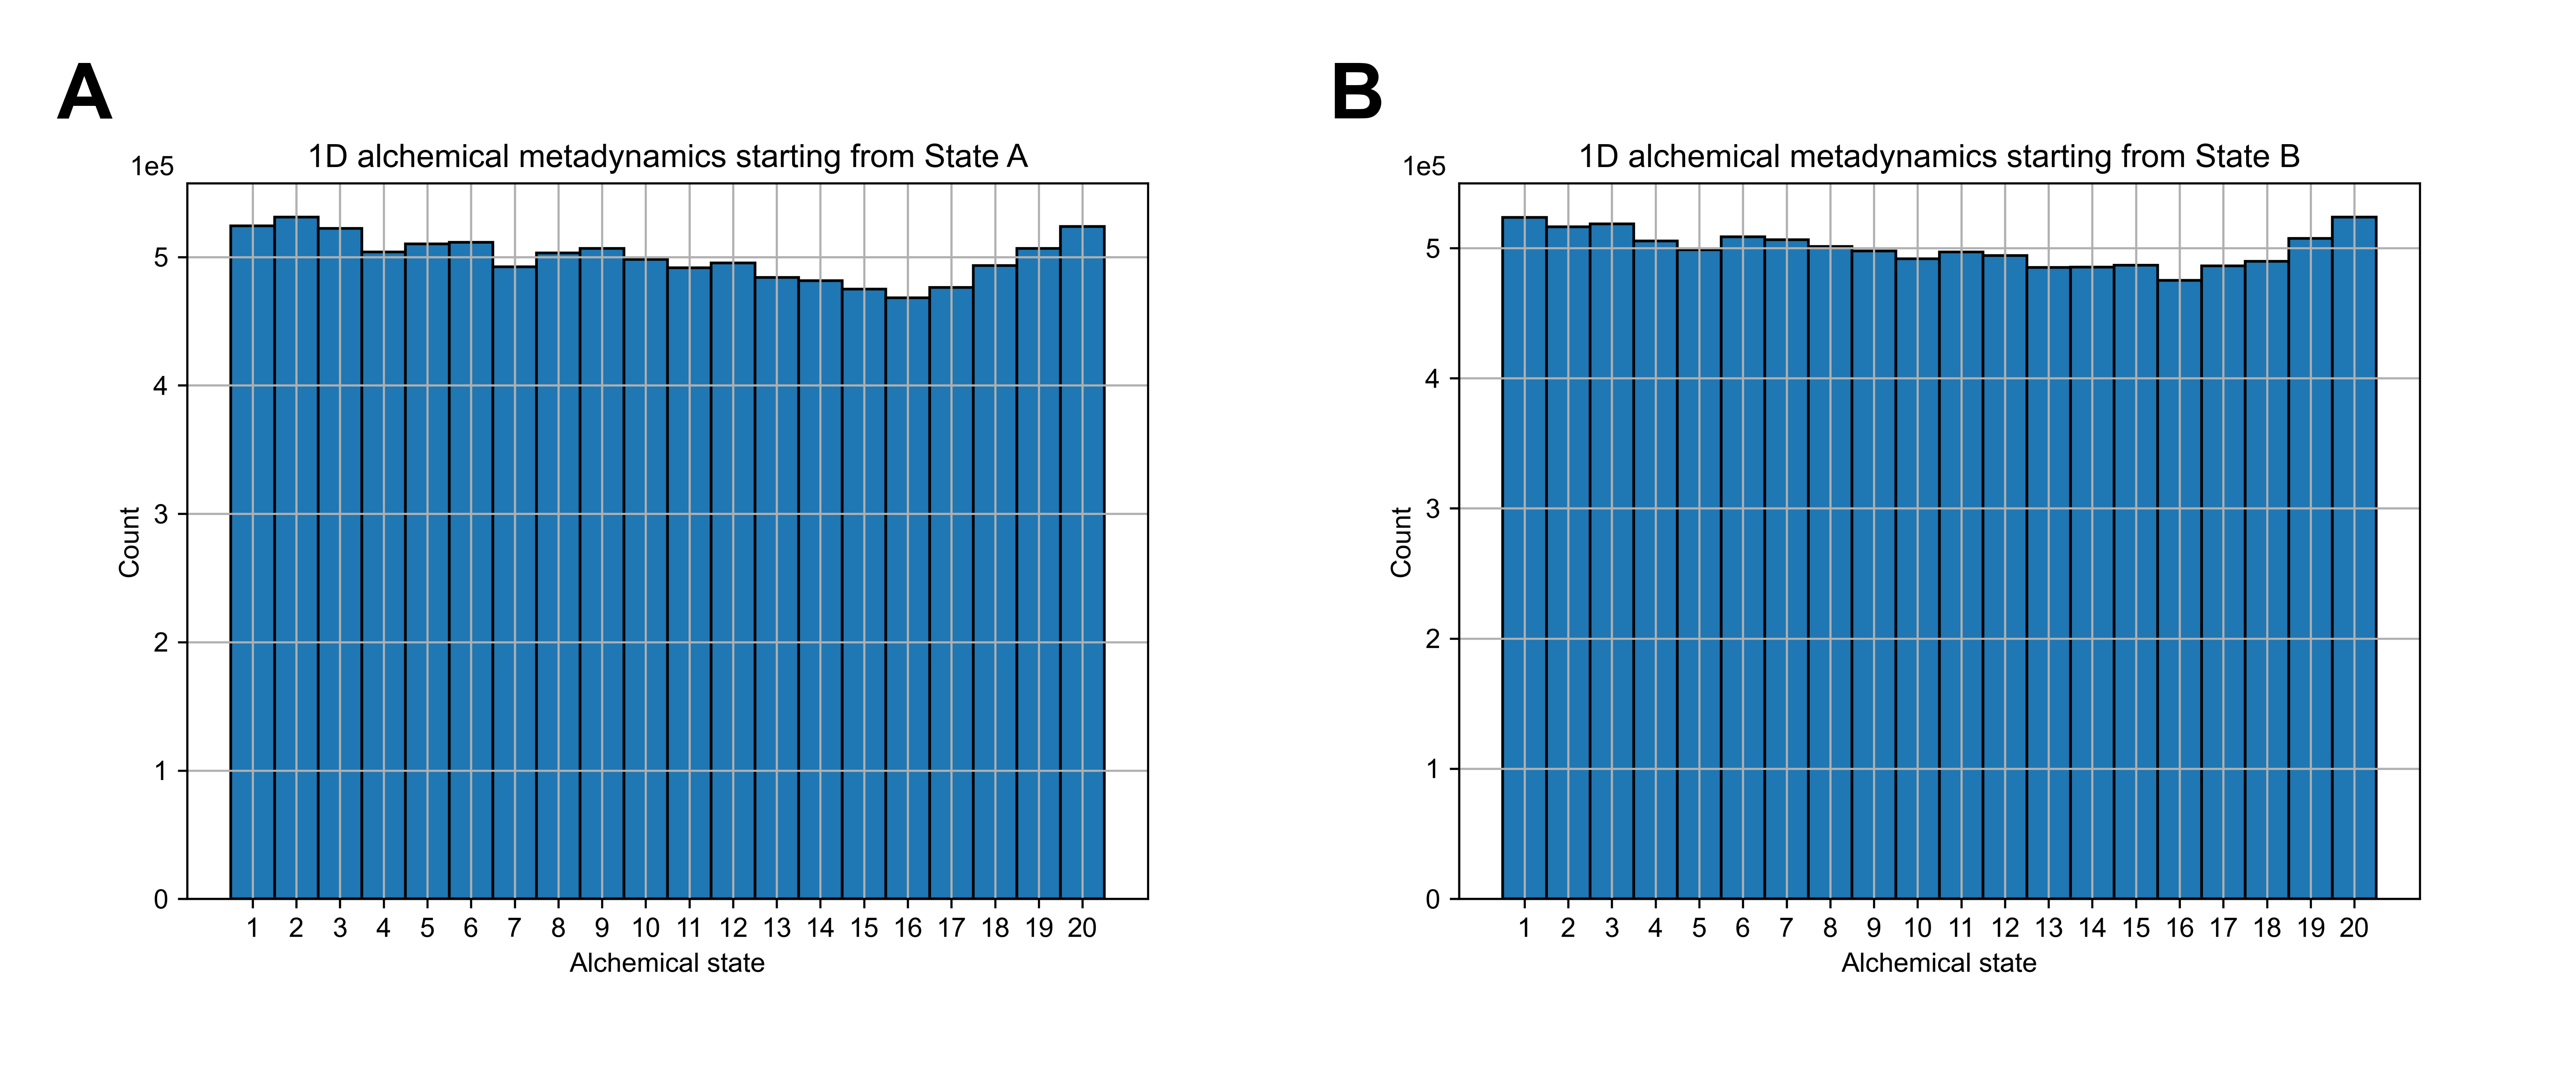
\includegraphics[width=\textwidth]{Figures/1D_lambda_hist.png}   
    \caption{The histograms of the state visitation in the 1D alchemical metadynamics starting from (A) State A and (B) State B. Both simulations were able to freely sample the alchemical space.}
    \label{sys2_1D_hist}
\end{figure}

\renewcommand{\thefigure}{S\arabic{figure}}
\begin{figure}[H]
    \centering
    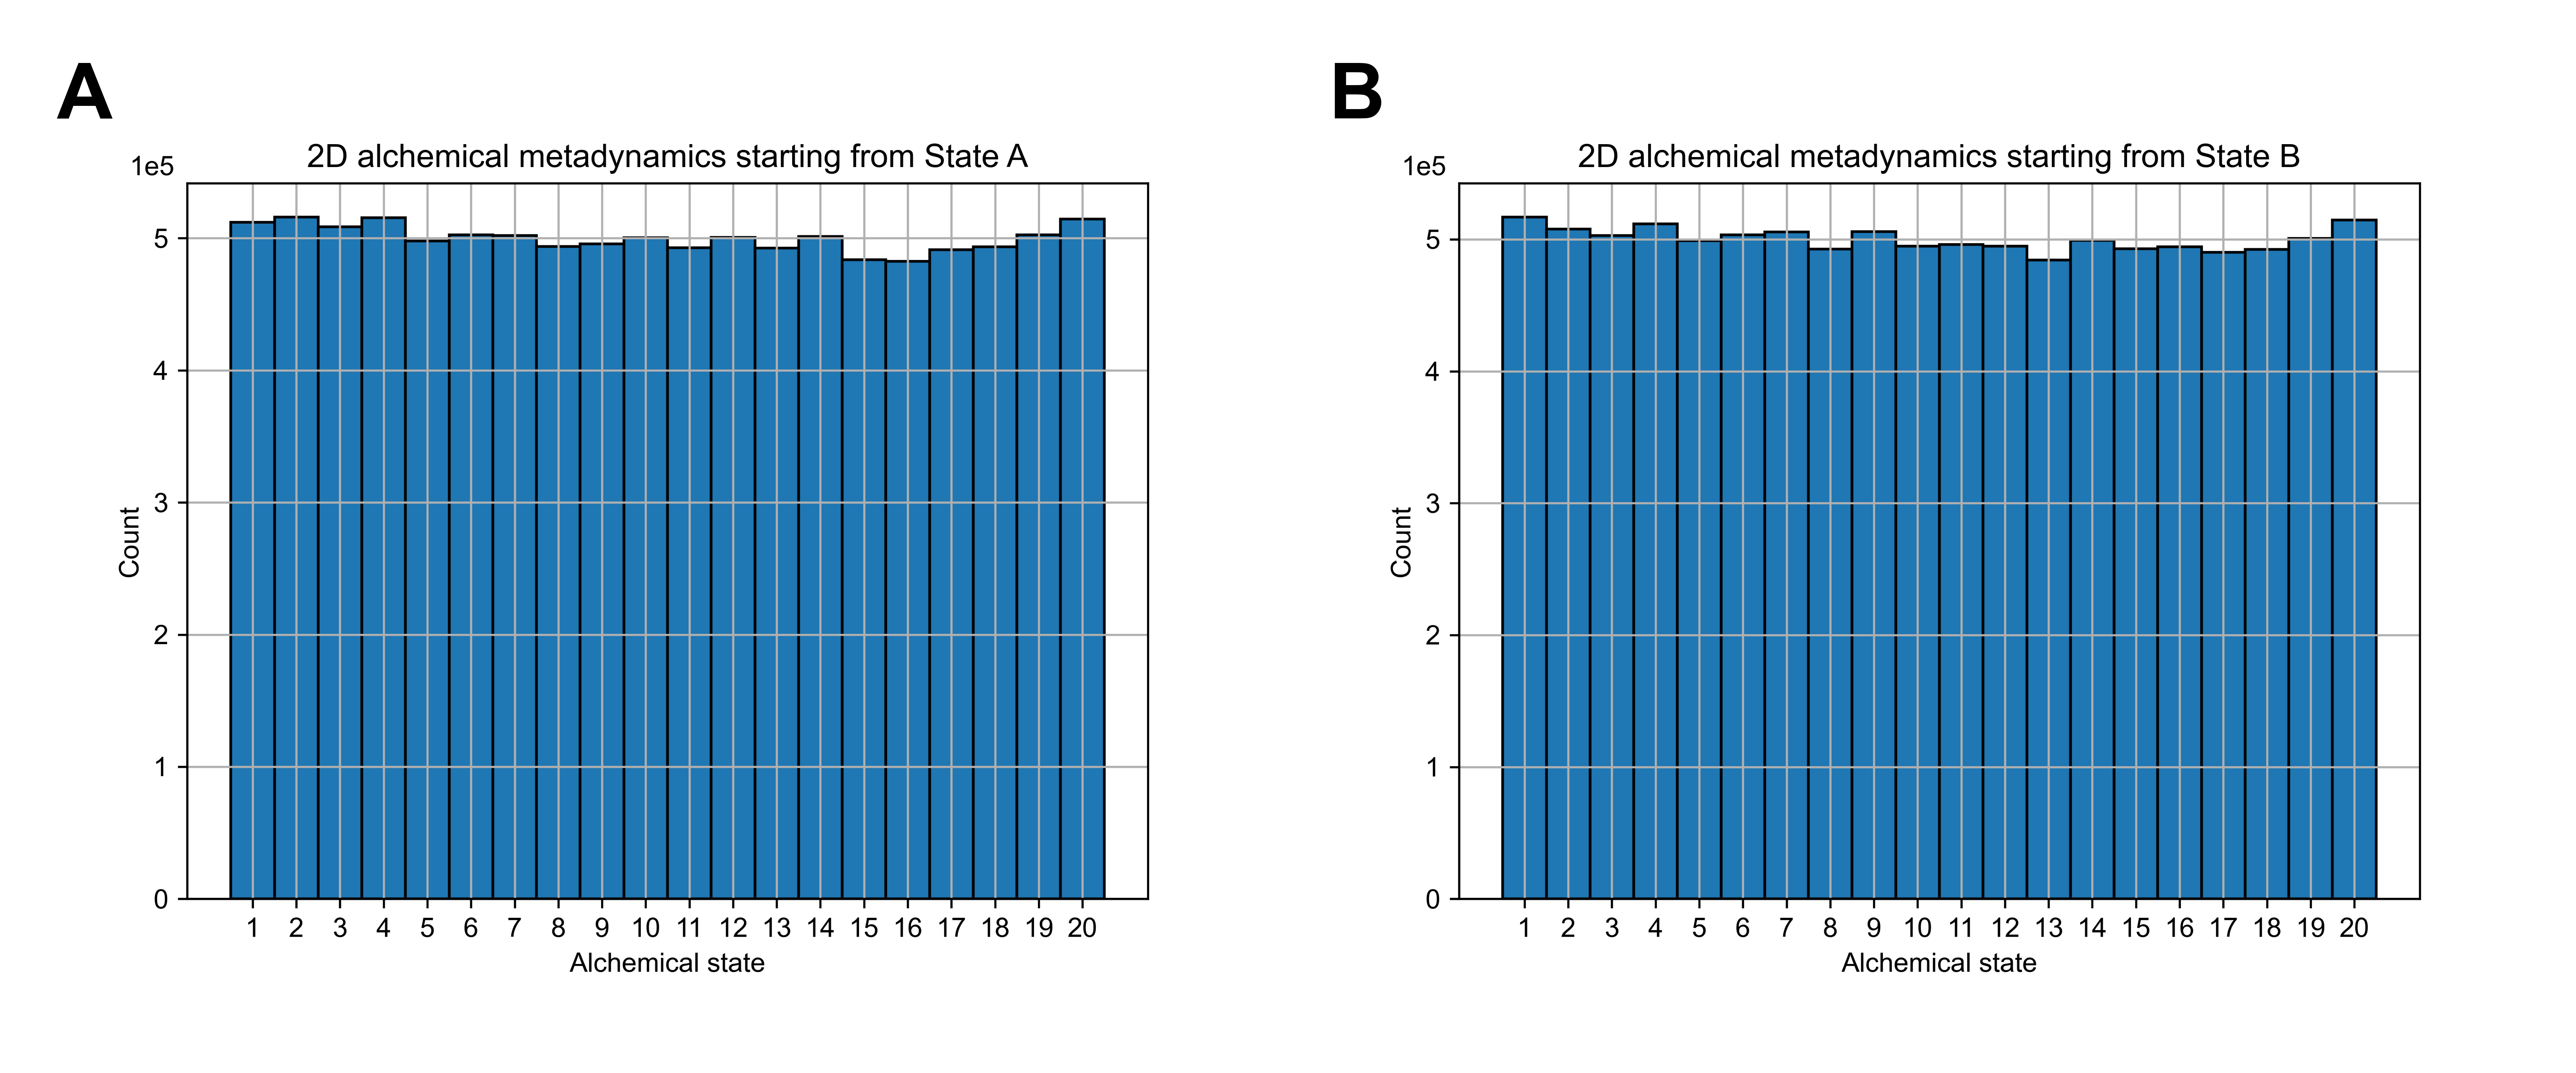
\includegraphics[width=\textwidth]{Figures/2D_lambda_hist.png}   
    \caption{The histograms of the state visitation in the 2D alchemical metadynamics starting from (A) State A and (B) State B. Similar to the two 1D simulations of System 2, both 2D simulations were able to freely sample the alchemical space.}
    \label{sys2_2D_hist}
\end{figure}

\renewcommand{\thefigure}{S\arabic{figure}}
\begin{figure}[H]
    \centering
    \includegraphics[width=\textwidth]{Figures/m6A_sampling.jpg}   
    \caption{(A) Value of the torsional angle N1-C6-N6-C10 as a function of time when the same torsional is used as CV, in a simulation performed at dynamic bias potential. In the 160 ns of simulations, the system only switches once from syn to anti state after about 8 ns and then back to syn after about 60 ns (B) Value of the torsional angle N1-C6-N6-C10 as a function of time when an averaged torsion between  N1-C6-N6-C10,  N1-C6-N6-H62, and  N1-C6-N6-H61 ($+ \pi$) is used as biasing collective variable. In this case, the system becomes diffusive on  N1-C6-N6-C10 after a few ns (C)  N1-C6-N6-C10 vs  N1-C6-N6-H62 when  N1-C6-N6-C10 is used as CV (D) N1-C6-N6-C10 vs  N1-C6-N6-H62 when the averaged torsion is used as CV. The three torsions mentioned here are coupled by an improper torsion that maintains the group C10, N6, H61, and H62 planar. The results shown here demonstrate that the improper torsion is not sufficiently stiff to maintain the consistency between the three torsions when enforcing the barrier crossing. As a consequence, the single N1-C6-N6-C10 torsion is not an optimal CV to allow a proper sampling of the torsional space.}
    \label{sampling}
\end{figure}


\clearpage
%\bibliography{refs}
\documentclass[journal=jacsat,manuscript=article]{achemso}

%%%%%%%%%%%%%%%%%%%%%%%%%%%%%%%%%%%%%%%%%%%%%%%%%%%%%%%%%%%%%%%%%%%%%
%% Place any additional packages needed here.  Only include packages
%% which are essential, to avoid problems later. Do NOT use any
%% packages which require e-TeX (for example etoolbox): the e-TeX
%% extensions are not currently available on the ACS conversion
%% servers.
%%%%%%%%%%%%%%%%%%%%%%%%%%%%%%%%%%%%%%%%%%%%%%%%%%%%%%%%%%%%%%%%%%%%%
\usepackage[version=3]{mhchem} % Formula subscripts using \ce{}

%%%%%%%%%%%%%%%%%%%%%%%%%%%%%%%%%%%%%%%%%%%%%%%%%%%%%%%%%%%%%%%%%%%%%
%% If issues arise when submitting your manuscript, you may want to
%% un-comment the next line.  This provides information on the
%% version of every file you have used.
%%%%%%%%%%%%%%%%%%%%%%%%%%%%%%%%%%%%%%%%%%%%%%%%%%%%%%%%%%%%%%%%%%%%%
%%\listfiles

%%%%%%%%%%%%%%%%%%%%%%%%%%%%%%%%%%%%%%%%%%%%%%%%%%%%%%%%%%%%%%%%%%%%%
%% Place any additional macros here.  Please use \newcommand* where
%% possible, and avoid layout-changing macros (which are not used
%% when typesetting).
%%%%%%%%%%%%%%%%%%%%%%%%%%%%%%%%%%%%%%%%%%%%%%%%%%%%%%%%%%%%%%%%%%%%%
\newcommand*\mycommand[1]{\texttt{\emph{#1}}}
\newcommand{\bfv}[1]{{\mbox{\boldmath{$#1$}}}}
\newcommand{\x}{\bfv{x}}
\usepackage{xr}
\makeatletter
\newcommand*{\addFileDependency}[1]{% argument=file name and extension
  \typeout{(#1)}
  \@addtofilelist{#1}
  \IfFileExists{#1}{}{\typeout{No file #1.}}
}
\makeatother

\newcommand*{\myexternaldocument}[1]{%
    \externaldocument{#1}%
    \addFileDependency{#1.tex}%
    \addFileDependency{#1.aux}%
}

\myexternaldocument{main}
%%%%%%%%%%%%%%%%%%%%%%%%%%%%%%%%%%%%%%%%%%%%%%%%%%%%%%%%%%%%%%%%%%%%%
%% Meta-data block
%% ---------------
%% Each author should be given as a separate \author command.
%%
%% Corresponding authors should have an e-mail given after the author
%% name as an \email command. Phone and fax numbers can be given
%% using \phone and \fax, respectively; this information is optional.
%%
%% The affiliation of authors is given after the authors; each
%% \affiliation command applies to all preceding authors not already
%% assigned an affiliation.
%%
%% The affiliation takes an option argument for the short name.  This
%% will typically be something like "University of Somewhere".
%%
%% The \altaffiliation macro should be used for new address, etc.
%% On the other hand, \alsoaffiliation is used on a per author basis
%% when authors are associated with multiple institutions.
%%%%%%%%%%%%%%%%%%%%%%%%%%%%%%%%%%%%%%%%%%%%%%%%%%%%%%%%%%%%%%%%%%%%%
\author{Wei-Tse Hsu}
\affiliation{Department of Chemical and Biological Engineering, University of Colorado Boulder, Boulder, CO 80305}
\author{Valerio Piomponi}
\affiliation{Scuola Internazionale Superiore di Studi Avanzati, Trieste, Italy}
\author{Pascal T. Merz}
\affiliation{Department of Chemical and Biological Engineering, University of Colorado Boulder, Boulder, CO 80305}
\author{Giovanni Bussi}
\affiliation{Scuola Internazionale Superiore di Studi Avanzati, Trieste, Italy}
\author{Michael R. Shirts}
\affiliation{Department of Chemical and Biological Engineering, University of Colorado Boulder, Boulder, CO 80305}
\email{michael.shirts@colorado.edu}

%%%%%%%%%%%%%%%%%%%%%%%%%%%%%%%%%%%%%%%%%%%%%%%%%%%%%%%%%%%%%%%%%%%%%
%% The document title should be given as usual. Some journals require
%% a running title from the author: this should be supplied as an
%% optional argument to \title.
%%%%%%%%%%%%%%%%%%%%%%%%%%%%%%%%%%%%%%%%%%%%%%%%%%%%%%%%%%%%%%%%%%%%%
\title
  {Supporting Information: Adding alchemical variables to metadynamics to enhance sampling in free energy calculations}

%%%%%%%%%%%%%%%%%%%%%%%%%%%%%%%%%%%%%%%%%%%%%%%%%%%%%%%%%%%%%%%%%%%%%
%% Some journals require a list of abbreviations or keywords to be
%% supplied. These should be set up here, and will be printed after
%% the title and author information, if needed.
%%%%%%%%%%%%%%%%%%%%%%%%%%%%%%%%%%%%%%%%%%%%%%%%%%%%%%%%%%%%%%%%%%%%%
% \abbreviations{IR,NMR,UV}
%\keywords{American Chemical Society, \LaTeX}

%%%%%%%%%%%%%%%%%%%%%%%%%%%%%%%%%%%%%%%%%%%%%%%%%%%%%%%%%%%%%%%%%%%%%
%% The manuscript does not need to include \maketitle, which is
%% executed automatically.
%%%%%%%%%%%%%%%%%%%%%%%%%%%%%%%%%%%%%%%%%%%%%%%%%%%%%%%%%%%%%%%%%%%%%
\begin{document}

% \clearpage
\section{Comparison of methylation free energy calculations with dynamic and static biases}
% We should include the lengths of the simulations using the dynamic bias and mention the adopted truncation fraction, average fraction, number of blocks in block bootstrapping, number of iteration for each data point. We should also explain the meaning of the 4th point by explicitly stating what values the 4th point took the difference from. (Like what is done in the section of free energy calculations for the last system in the main text.) 
As a supplementary information, we show the free energy calculations with dynamic bias for the nucleotide and duplex systems. These calculations are done in comparison with the free energy differences computed with static bias presented in the main text. Specifically, simulations at dynamic bias were elongated up to 160 ns. For analysis, the first 60 ns were discarded, and the bias averaged over the remaining 100 ns was used to compute weights. Different numbers of blocks ranging 2 to 1000 were used to construct histograms in block boostrapping (200 iterations) and the largest uncertainty is reported. 

The figure below shows that with dynamic bias, the free energy estimates are more precise (lower statistical errors). This is mostly likely  attributable to the fact that the sampling in the CV space is more diffusive in these systems with dynamically updated weights. However, free energy estimates computed with dynamic bias are less accurate, i.e. the results differ more in alchemical metadynamics than in the case of Hamiltonian replica exchange (HREX). This is probably caused by the dynamic bias adding some small amount of history-dependent blurring. 

To further demonstrate the lower accuracy of the dynamic bias computation, the free energy difference ($\Delta G^{\text{dup, A}}_{syn/anti}$) between the two conformations of adenosine shown in Figure 3A in the main text is calculated. In the work by Piomponi et al.,~\cite{piomponi2022molecular} this value was assumed to be 0 because of the symmetry of the hydrogen atoms H61 and H62. Also, HREX used in the previous work does not have the access to the free energy landscape along the biased torsion, so the relative error is not given for the HREX case. In alchemical metadynamics, $\Delta G^{\text{dup, A}}_{anti/syn}$ was calculated as follows: 
\begin{equation}
    \Delta G^{\text{dup, A}}_{syn/anti}=-\frac{1}{\beta} \ln \left( \frac{\sum_{i \in anti} e^{\beta V^{\text{dup}}_{\text{tot}}(\eta_i, \lambda=0) }}{\sum_{i \in syn} e^{\beta V^{\text{dup}}_{\text{tot}}(\eta_i, \lambda=0)}}\right )
\end{equation} 

For most systems, the general understanding is that using plain metadynamics instead of doing the two-step procedure is better~\cite{bussi2020using}. It is likely the result is system dependent and related to the fact that even without a dynamic bias we can see many of transitions, thus a reasonable statistical error. In this way, we are clearly in the regime where fewer transitions at equilibrium are a safer estimate.

\renewcommand{\thefigure}{S\arabic{figure}}
\begin{figure}[H]
    \centering
    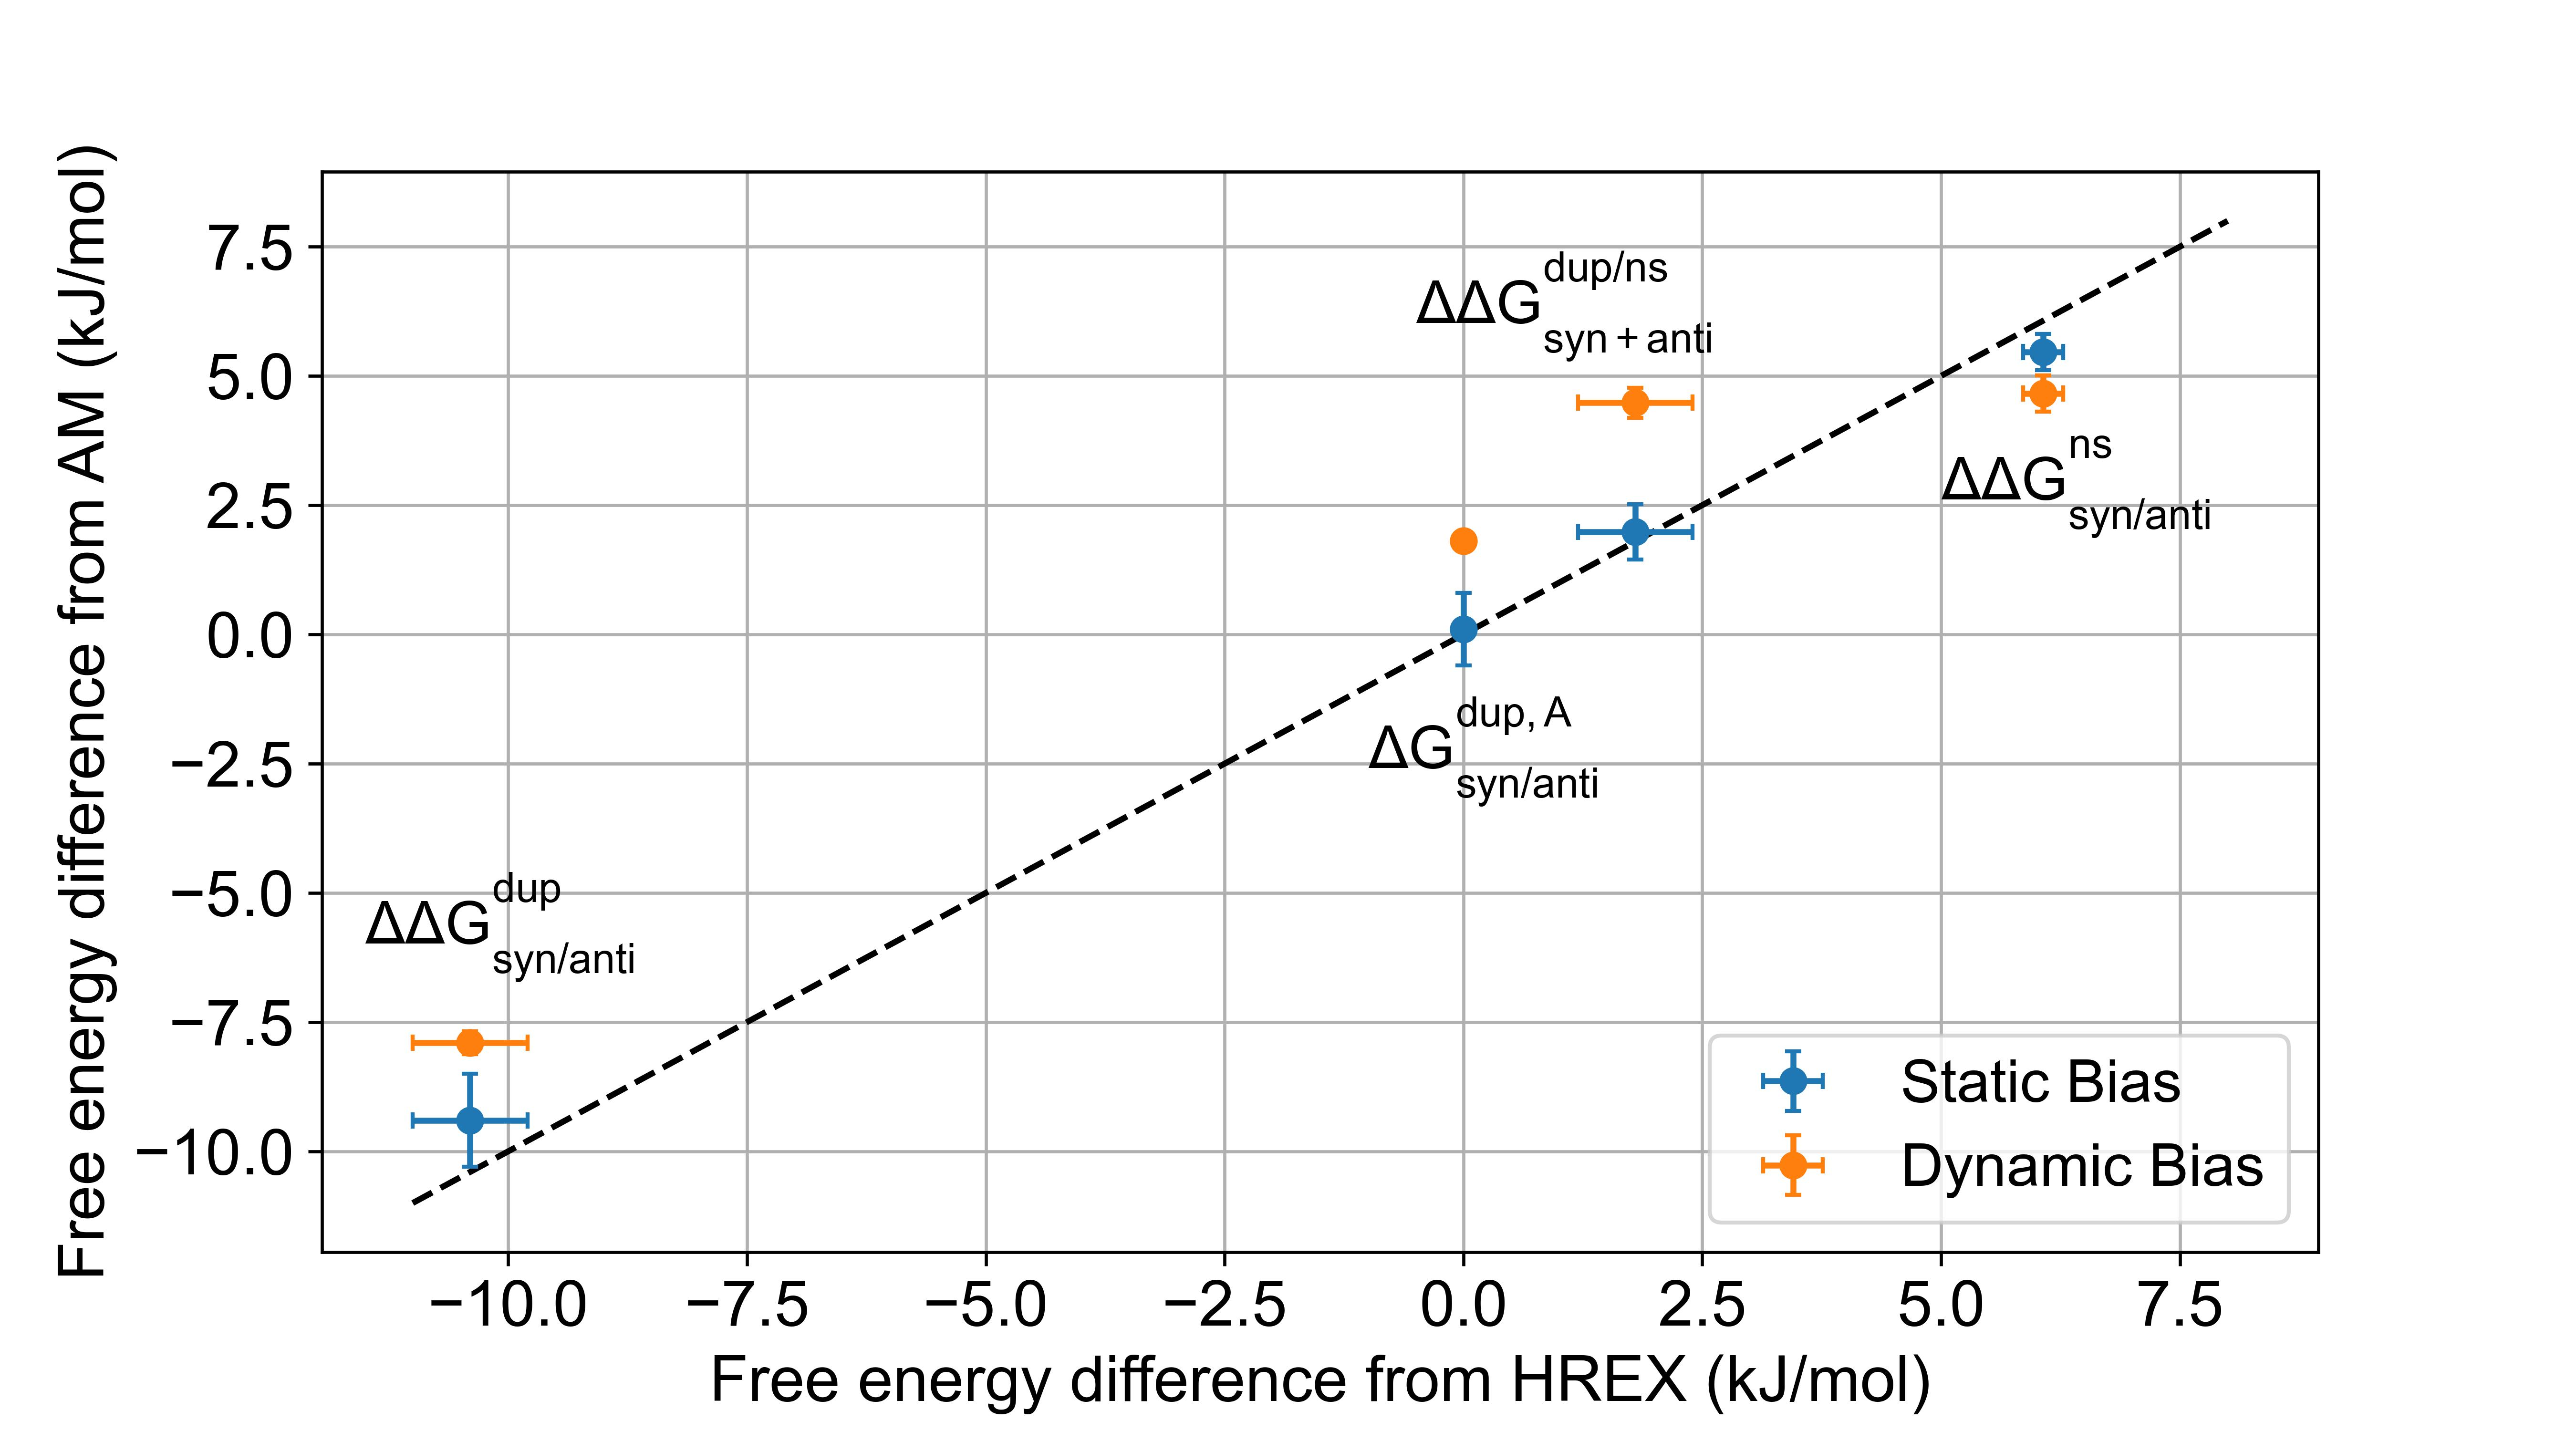
\includegraphics[width=\textwidth]{Figures/m6A_dynamic_static.jpg}   
    \caption{Comparison of free energy differences computed in Ref.~\cite{piomponi2022molecular} with Hamiltonian replica exchange (HREX) and $\Delta \Delta G$ computed with alchemical metadynamics (AM) in this work, for two cases: (1) static bias (as discussed in the main text) and (2) dynamic bias.}
    \label{compare_ACS}
\end{figure}

\section{Supplementary Figures}
\renewcommand{\thefigure}{S\arabic{figure}}
\begin{figure}[H]
    \centering
    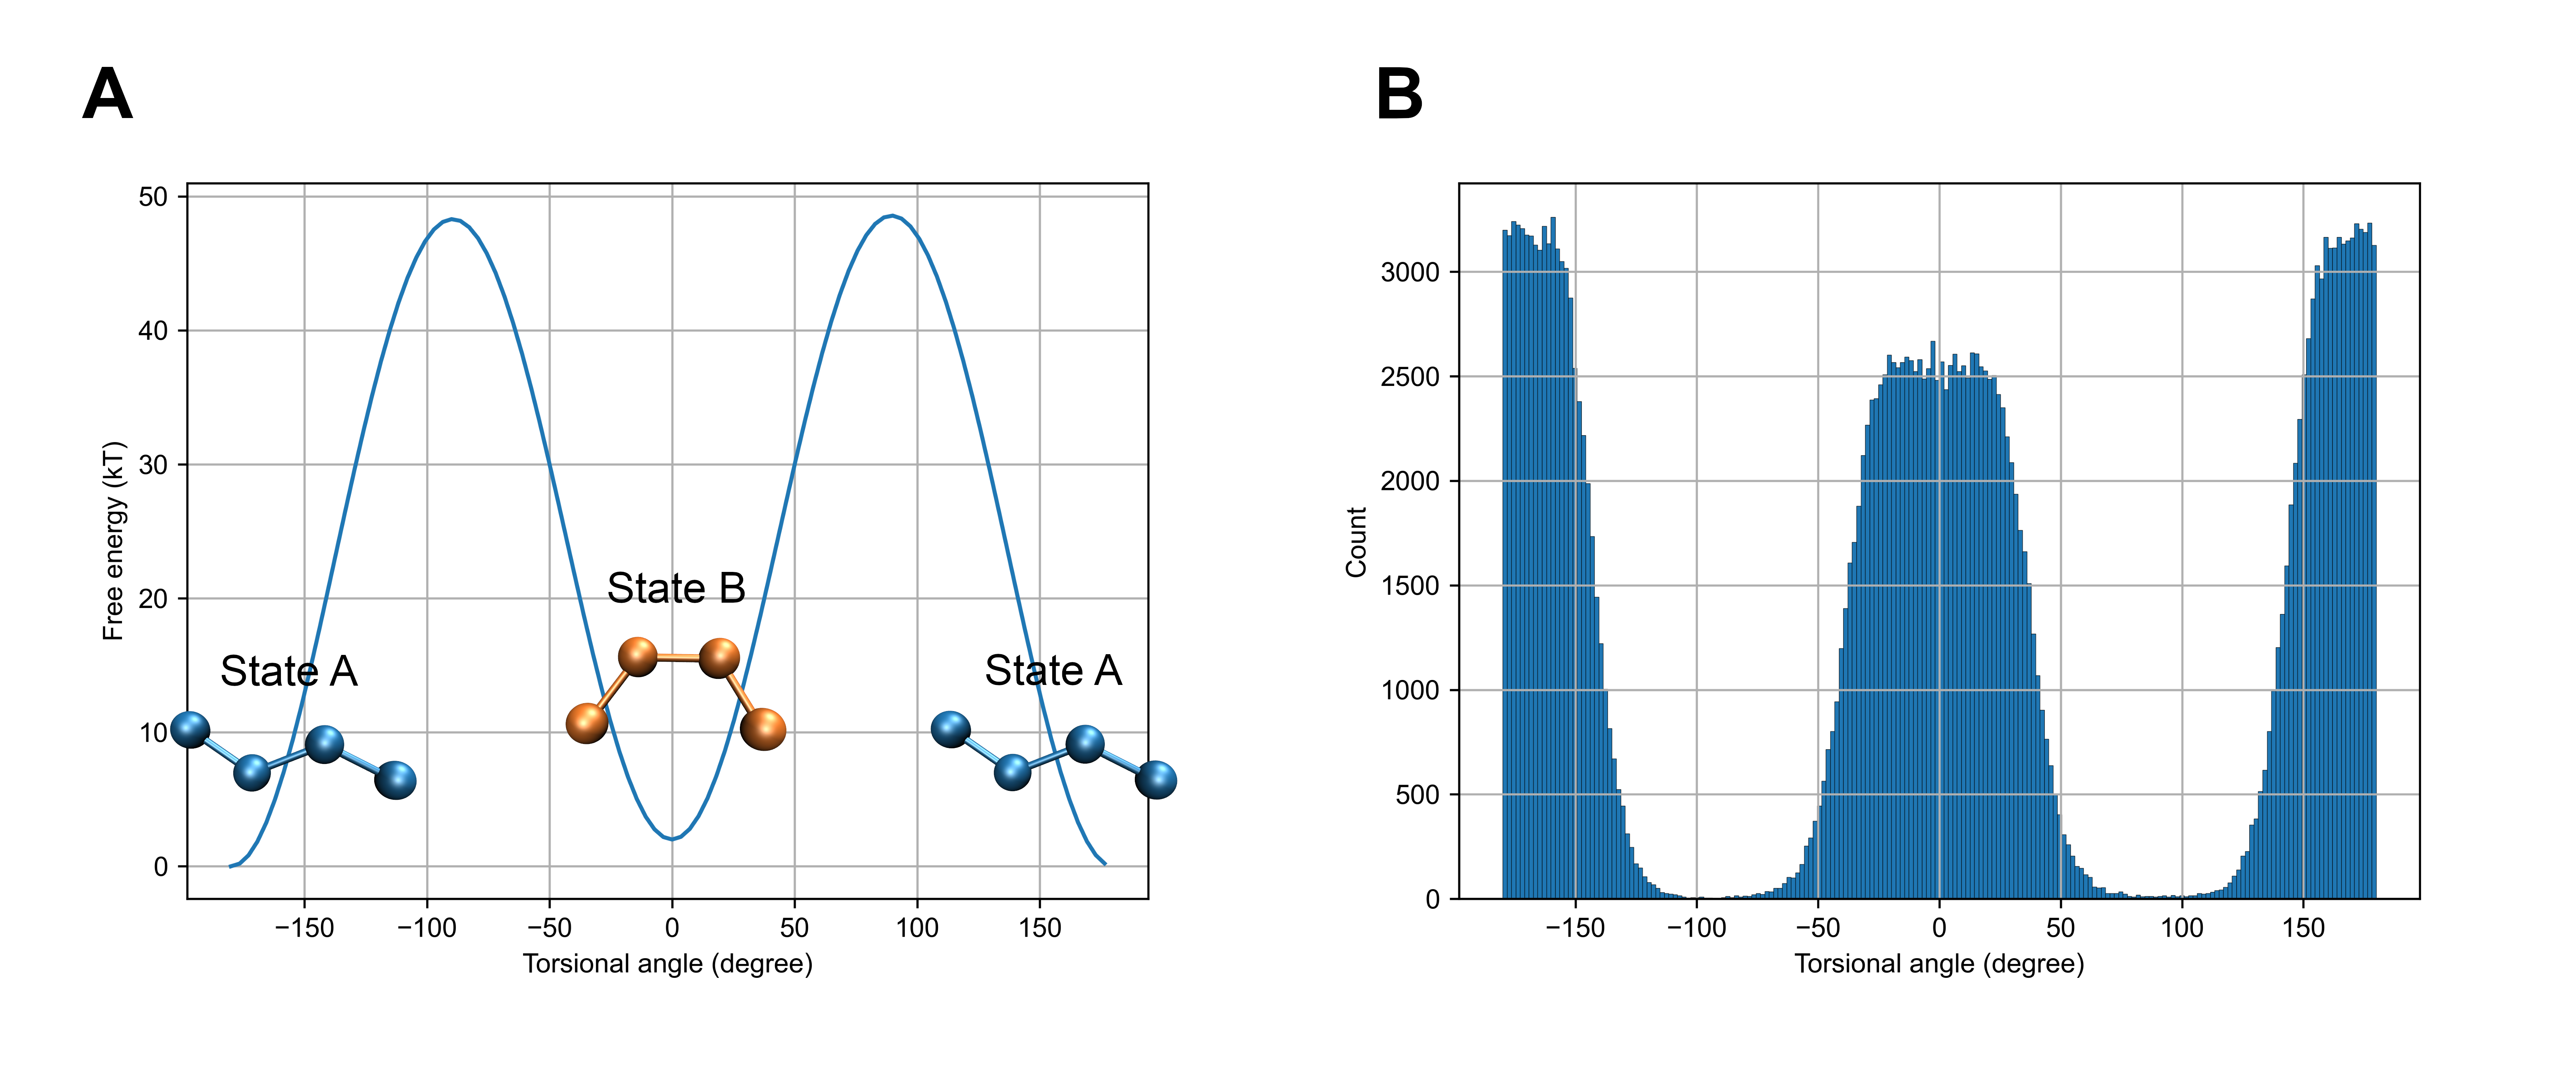
\includegraphics[width=\textwidth]{Figures/sys2_torsional_MetaD_annotated.png}   
    \caption{(A) The free energy profile as a function of the torsional angle. We refer the structures have a torsional angle of $\pm$180$^{\circ}$ and 0$^{\circ}$ as State A (trans isomer) and State B (cis isomer). The torsional free energy barrier starting from either state is around 48.56 kT, which might not be exact since the analysis was done on a very short (5 ns) simulation solely for generating configurations at both states. (B) The histogram of the sampled torsional angle in the torsional metadynamics. As can be seen, the system was able to sample both states frequently during the short simulation.}
    \label{sys2_torsional_MetaD}
\end{figure}

\renewcommand{\thefigure}{S\arabic{figure}}
\begin{figure}[H]
    \centering
    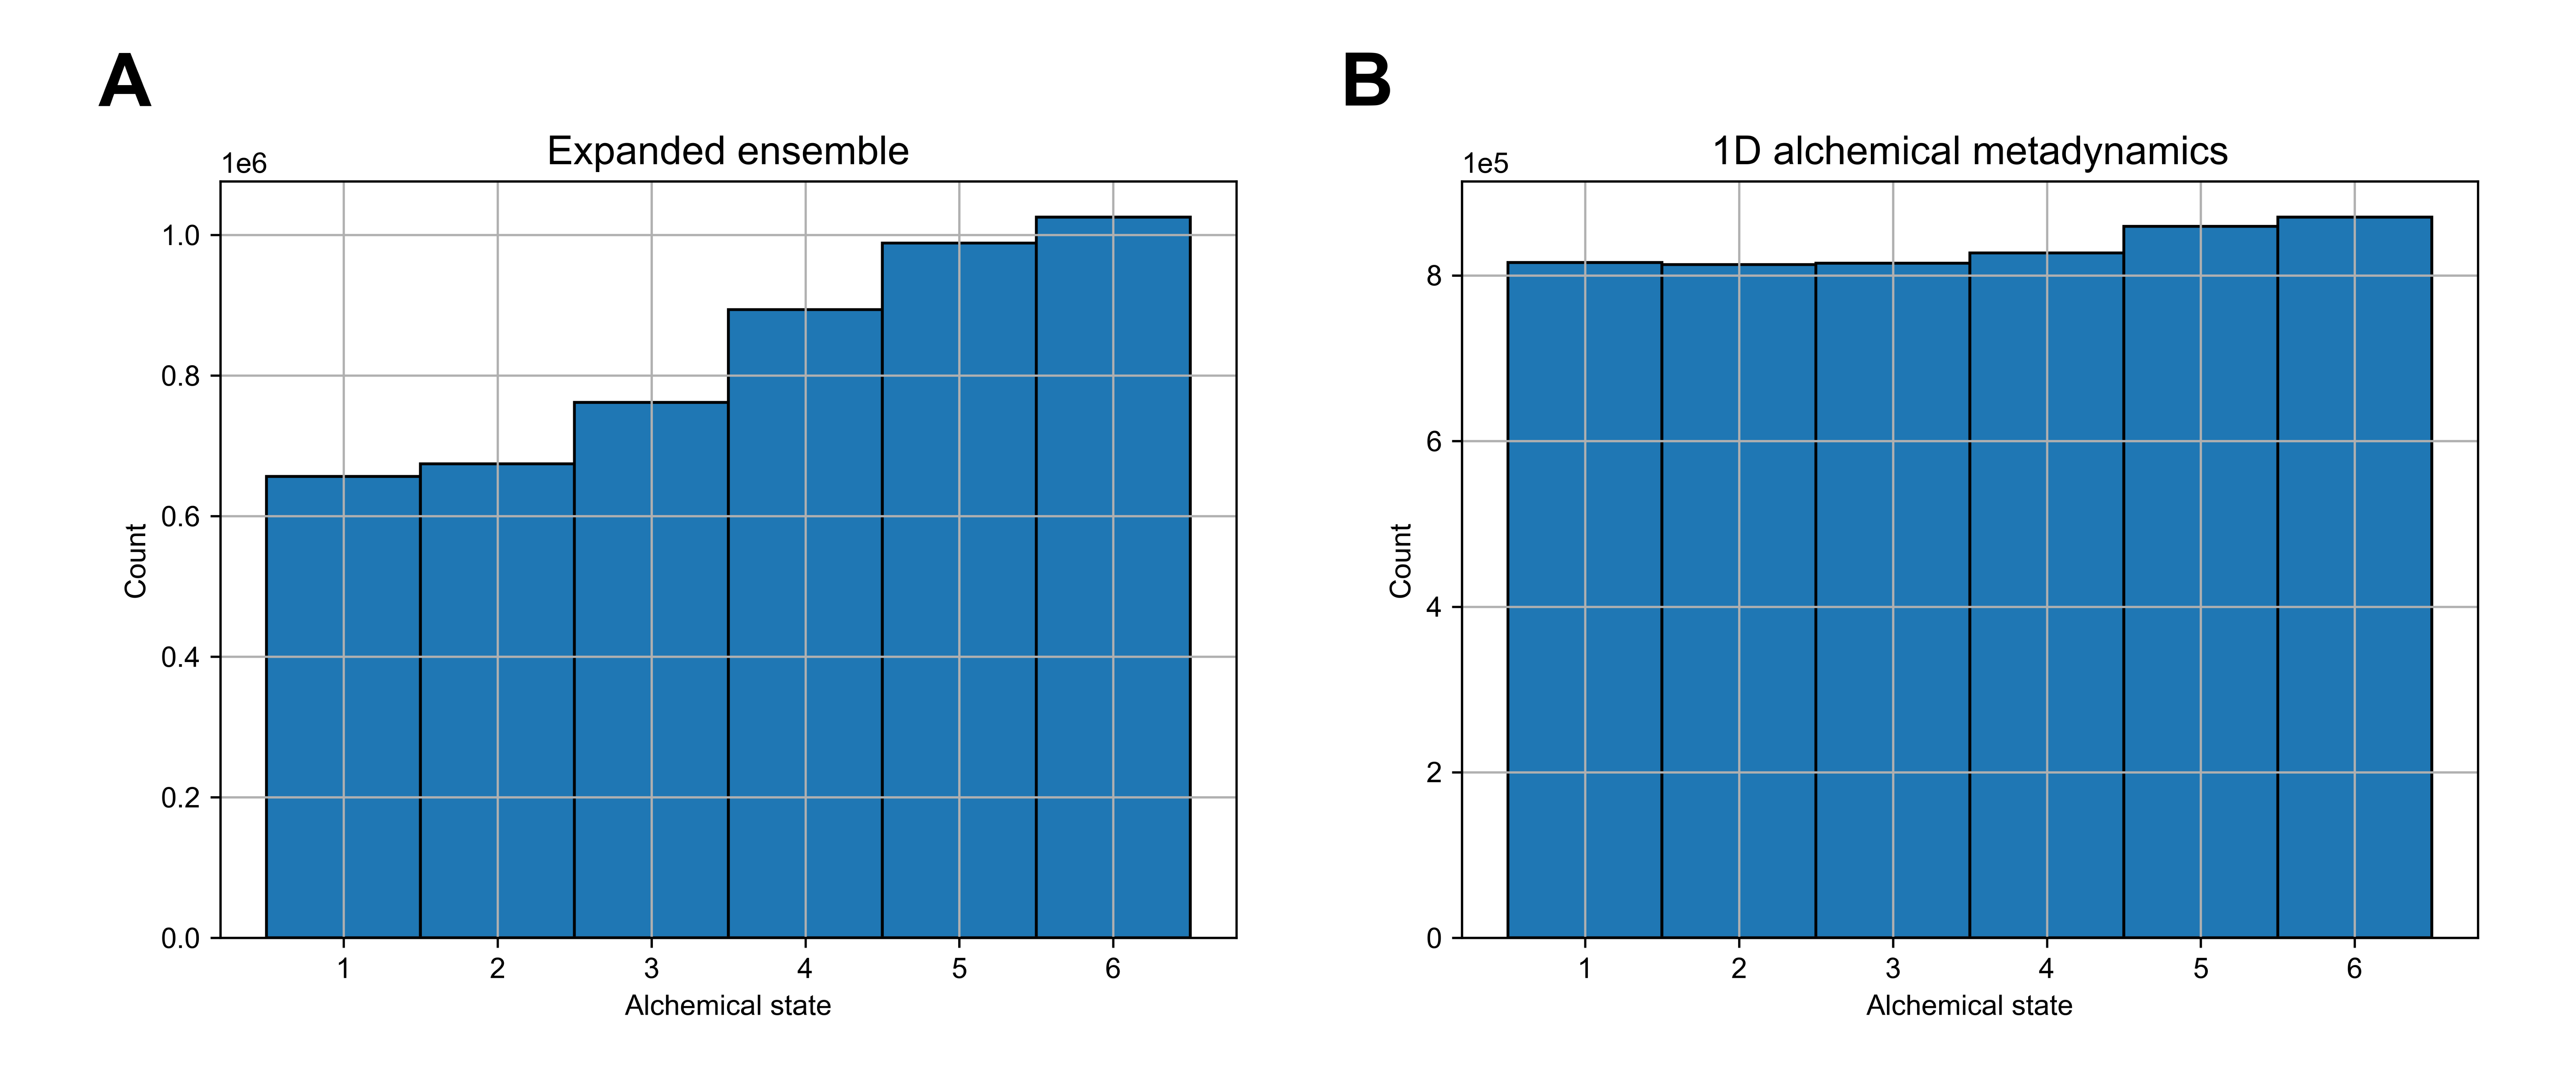
\includegraphics[width=\textwidth]{Figures/sys1_histograms.png}   
    \caption{The histograms of the state visitation in (A) expanded ensemble and (B) 1D alchemical metadynamics of System 1. Both simulations were able to sample all the intermediate states frequently.}
    \label{sys1_hist}
\end{figure}

\renewcommand{\thefigure}{S\arabic{figure}}
\begin{figure}[H]
    \centering
    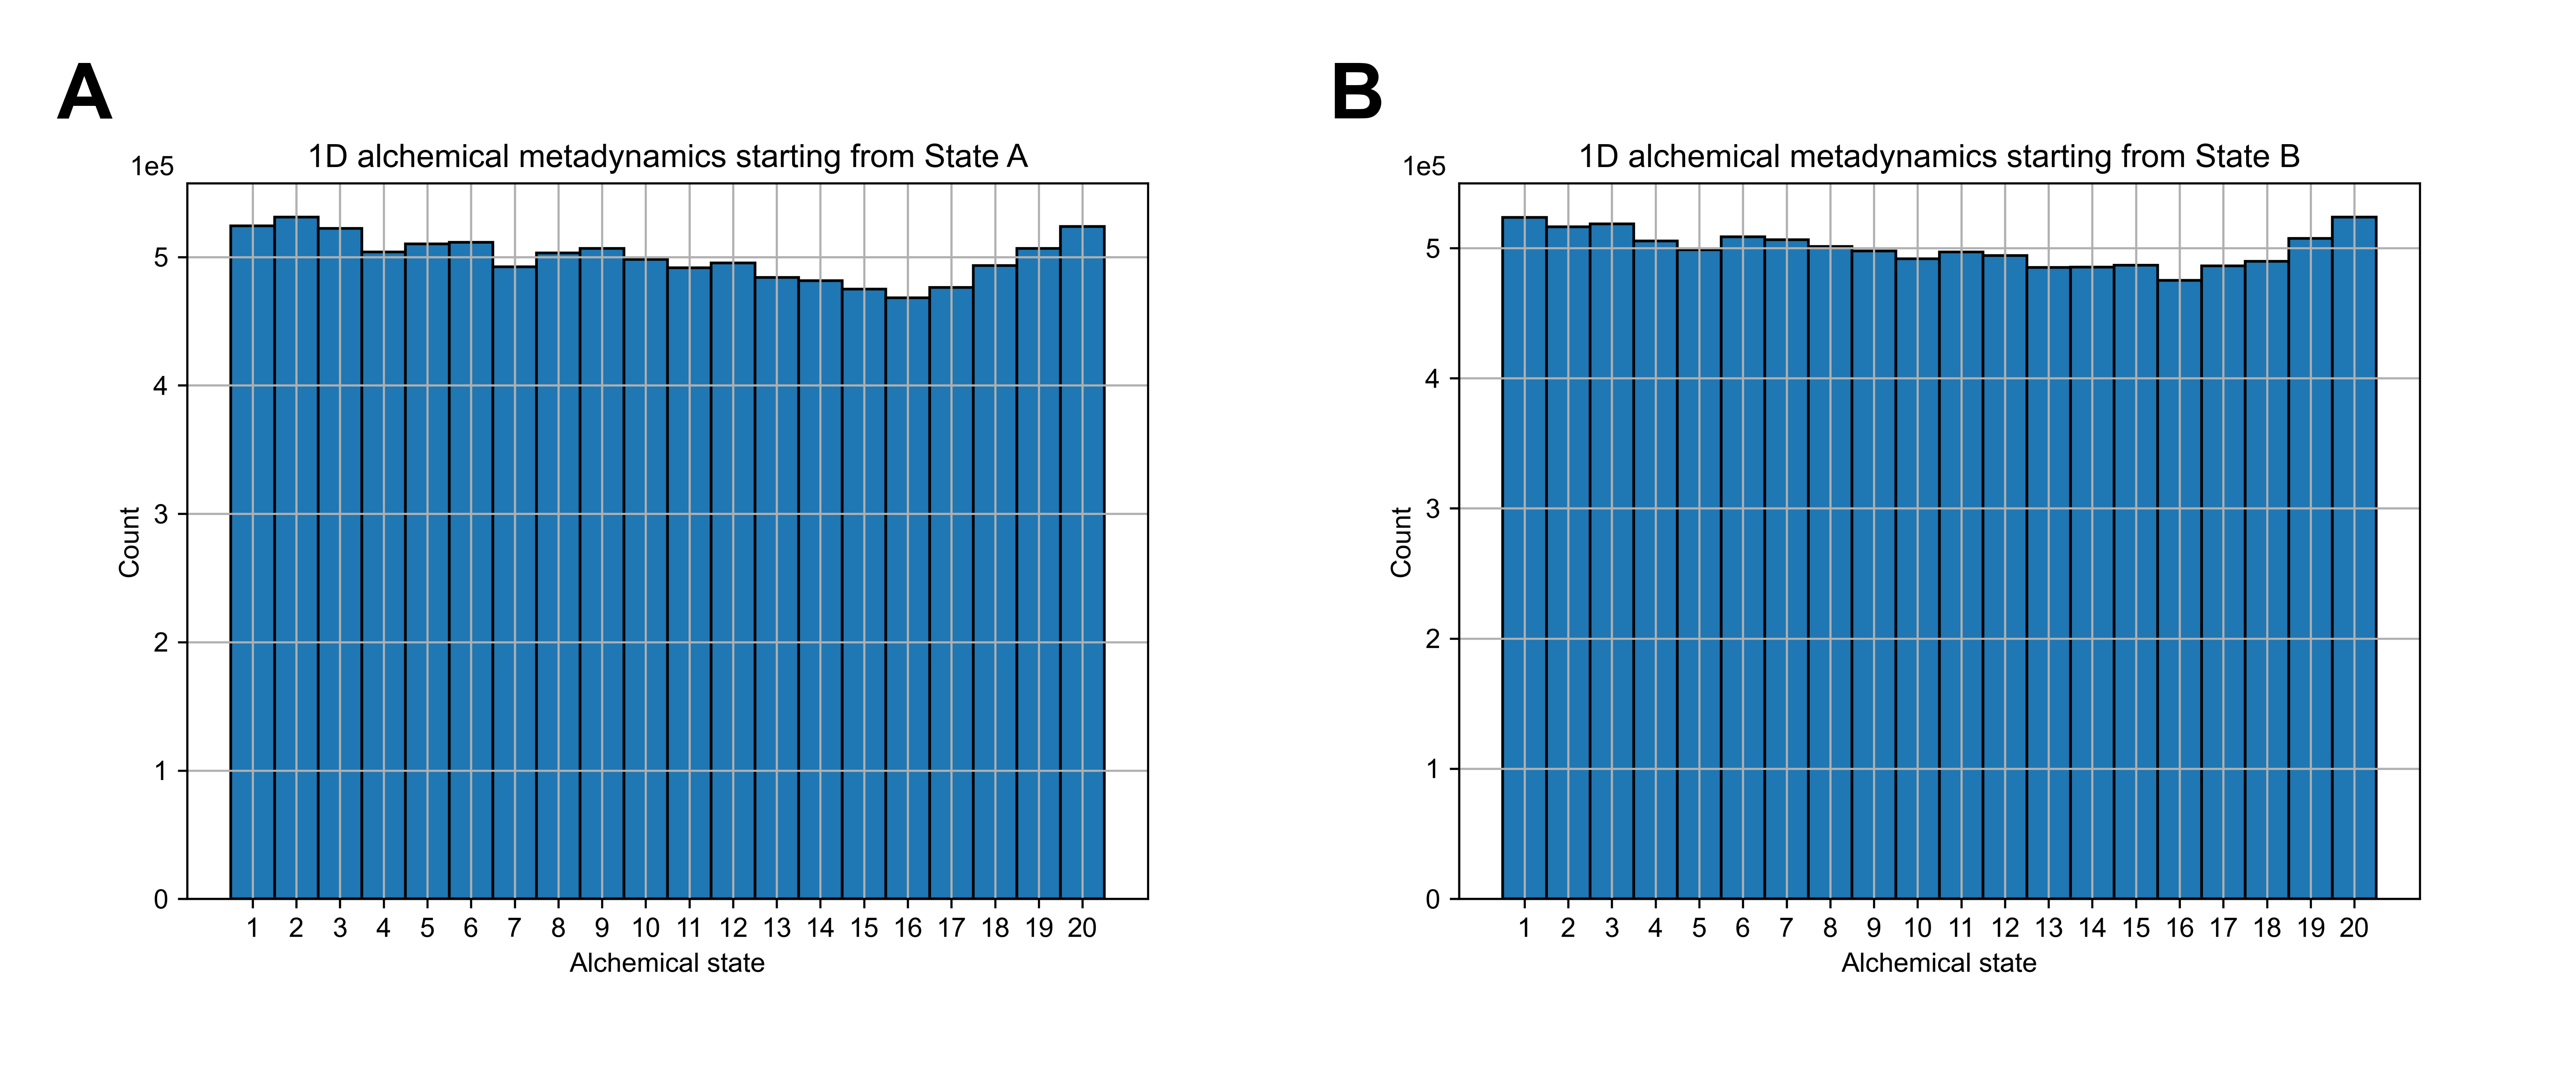
\includegraphics[width=\textwidth]{Figures/1D_lambda_hist.png}   
    \caption{The histograms of the state visitation in the 1D alchemical metadynamics starting from (A) State A and (B) State B. Both simulations were able to freely sample the alchemical space.}
    \label{sys2_1D_hist}
\end{figure}

\renewcommand{\thefigure}{S\arabic{figure}}
\begin{figure}[H]
    \centering
    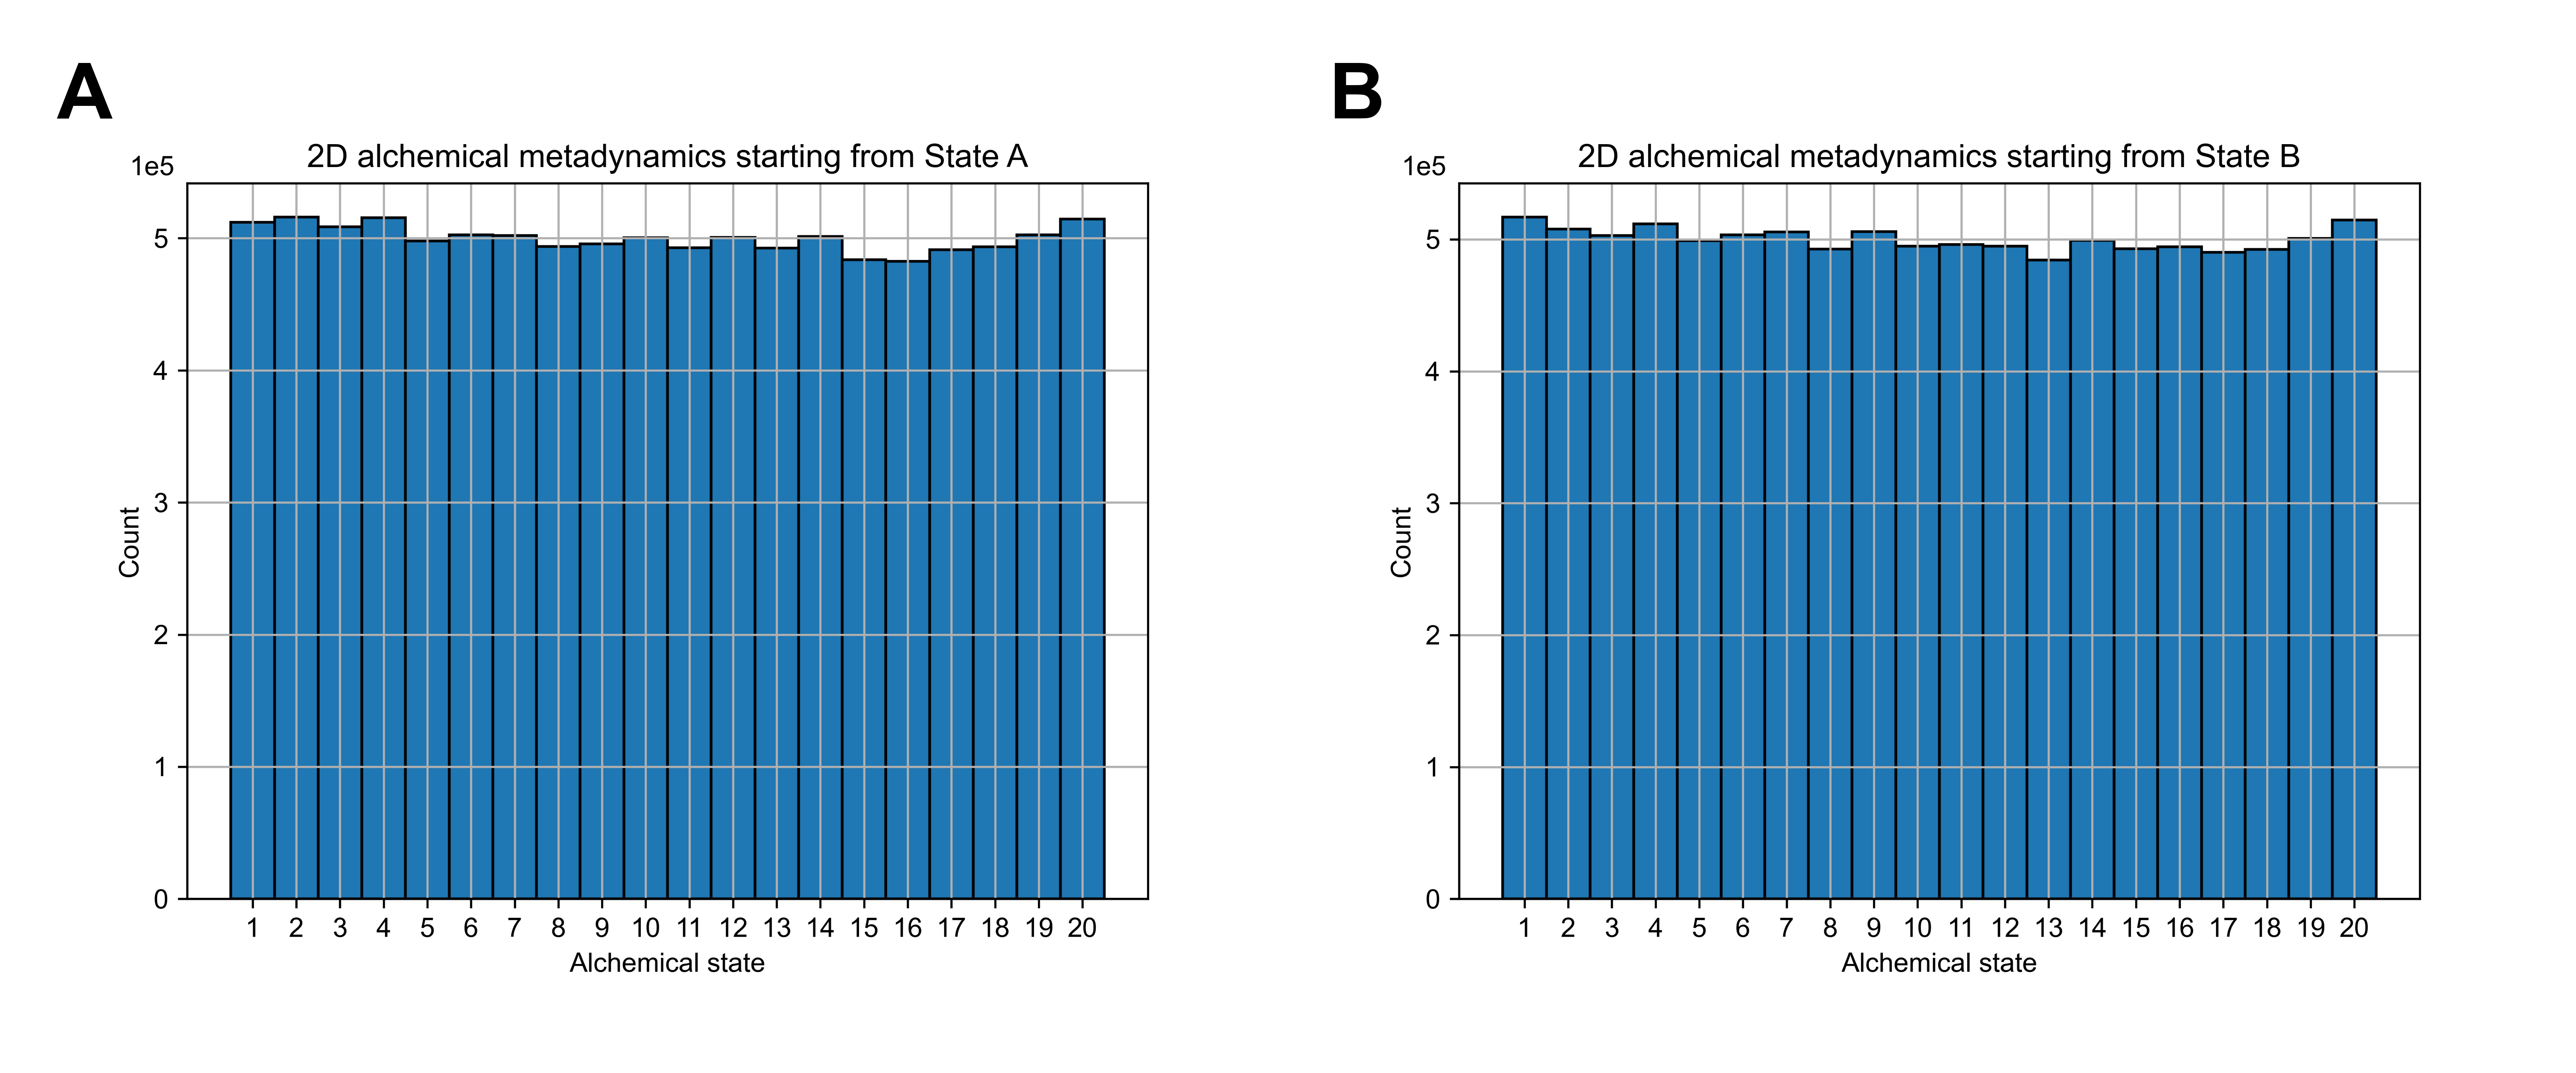
\includegraphics[width=\textwidth]{Figures/2D_lambda_hist.png}   
    \caption{The histograms of the state visitation in the 2D alchemical metadynamics starting from (A) State A and (B) State B. Similar to the two 1D simulations of System 2, both 2D simulations were able to freely sample the alchemical space.}
    \label{sys2_2D_hist}
\end{figure}

\renewcommand{\thefigure}{S\arabic{figure}}
\begin{figure}[H]
    \centering
    \includegraphics[width=\textwidth]{Figures/m6A_sampling.jpg}   
    \caption{(A) Value of the torsional angle N1-C6-N6-C10 as a function of time when the same torsional is used as CV, in a simulation performed at dynamic bias potential. In the 160 ns of simulations, the system only switches once from syn to anti state after about 8 ns and then back to syn after about 60 ns (B) Value of the torsional angle N1-C6-N6-C10 as a function of time when an averaged torsion between  N1-C6-N6-C10,  N1-C6-N6-H62, and  N1-C6-N6-H61 ($+ \pi$) is used as biasing collective variable. In this case, the system becomes diffusive on  N1-C6-N6-C10 after a few ns (C)  N1-C6-N6-C10 vs  N1-C6-N6-H62 when  N1-C6-N6-C10 is used as CV (D) N1-C6-N6-C10 vs  N1-C6-N6-H62 when the averaged torsion is used as CV. The three torsions mentioned here are coupled by an improper torsion that maintains the group C10, N6, H61, and H62 planar. The results shown here demonstrate that the improper torsion is not sufficiently stiff to maintain the consistency between the three torsions when enforcing the barrier crossing. As a consequence, the single N1-C6-N6-C10 torsion is not an optimal CV to allow a proper sampling of the torsional space.}
    \label{sampling}
\end{figure}


\clearpage
%\bibliography{refs}
\input{supporting_info.bbl}
\end{document}
\end{document}
\end{document}
\end{document}